\chapter{Atoms}
\label{chap05}

\section{Introduction}

In this chapter, we will examine the wavefunctions for the ground states 
of atoms.  A key idea is the Aufbau principle, which forms the basis for 
understanding chemical regularities of atoms.

Throughout this chapter, we will use atomic units of $\hbar = 1$, $| e | = 
1$, and $m_e = 1$.  Consequently, the unit of energy is $h_0 = 1$ 
hartree = 27.2116 $eV =$ 627.51 kcal/mole, and the unit of length is $a_0 = 
1$  bohr = 0.52918\AA.  First, we will examine the excited states of the H atom.

\section{Excited States H Atoms}

Rather than derive the eigenstates of the hydrogen atom, by standard techniques
of partial differential equations, we prefer to examine the qualitative 
reasons behind the forms of the solutions.  Although the Schr\"odinger equation
\begin{equation}
H \phi = E \phi
\end{equation}
can be solved for the H atom, it cannot for most other systems of interest, 
and hence, qualitative reasoning will be almost essential in most systems.

In atomc units
\begin{equation}
H = - {1 \over 2} \nabla^2 - {Z \over r} .
\label{chap5-eqno1}
\end{equation}
Because $H$ is independent of orientation, the exact eigenstates can 
be factored into a radial part $R(r)$, and an angular part $Z( \theta , 
\varphi)$
\begin{equation}
\phi ( r , \theta , \varphi ) = R ( r ) Z ( \theta , \varphi )
\end{equation}
where $z = r \cos \theta$, $x = r \sin \theta \cos \varphi$, and $y = r 
\sin \theta \sin \varphi$.

\subsection{Angular Functions}

From $H \phi = E \phi$, we obtain
\begin{equation}
E = \langle \phi | H | \phi \rangle = T + V,
\end{equation}
where, using atomic units, from (\ref{chap5-eqno1})
\begin{equation}
V = \langle \phi | - {Z \over r} | \phi \rangle
\end{equation}
and
\begin{equation}
T = - {1 \over 2} \langle | \nabla^2 | \phi \rangle = {1 \over 2} 
\langle | \nabla \phi |^2 \rangle.
\label{chap5-eqno2}
\end{equation}
Using spherical coordinates, $r, \theta , \varphi$, we will first fix the 
radial coordinate $r$ and examine functions of angular coordinates 
$\theta$, $\varphi$ only.

At fixed $r$, the potential energy $V$ is independent of angular coordinate 
and hence, it is the kinetic energy that is affected by the angular part 
of the wavefunction.  Since the kinetic energy is proportional to the 
average square of the gradient of the wavefunction, the best, lease energy, 
angular function is the smoothest, i.e., a constant
\begin{equation}
\phi_0 ( \theta , \varphi ) = 1.
\label{chap5-eqno3}
\end{equation} It is convenient to define an integer $l$ indicating the number of
angular nodal planes.  Later, $l$ will be referred to as the total
orbital angular momentum quantum number.  The function
(\ref{chap5-eqno3}) has the same sign for all $\theta$ and $\varphi$,
and hence, is $l = 0$.

All other angular functions must be orthogonal to (\ref{chap5-eqno3}),
and hence, all must have an equal number of positive and negative
regions, $l \geq 1$.  As the number of angular nodal planes, $l$
increases, the average square of the gradient increases, and hence,
the angular kinetic energy increases.  Thus, the angular functions
will be ordered as $l = 0, l = 1, l = 2$, and $l = 3$, etc.

There are three orthogonal functions, all having one nodal plane.  For example,
\begin{eqnarray}
\phi_z ( \theta , \varphi ) &=& {z \over r} = \cos \theta\cr
\phi_x ( \theta , \varphi ) &=& {x \over r} = \sin \theta \cos \varphi\cr
\phi_y ( \theta , \varphi ) &=& {y \over r} = \sin \theta \cos \varphi
\label{chap5-eqno4}
\end{eqnarray}
Any other function, with one nodal plane, and orthogonal to $l = 0$,
can be written as a linear combination of the functions in
(\ref{chap5-eqno4}).  It is easy to see that these functions are
orthogonal. For example,
\begin{equation}
\phi_z \phi_x = \left( {zx \over r^2} \right)
\end{equation}
leads to two nodal planes and phases as shown following

% YT?
%\centerline{{{\ithick=.8pt \othick=0pt \spacing=12pt \abovehr=18pt 
%\belowhr=20pt \nexttovr=30pt
%\table{z}-!+\rr +!-\caption{} }}}

\noindent
and hence, the angular integral,
\begin{equation}
\langle \phi_z | \phi_x \rangle = \int d \Omega \phi_z \phi_x ,
\end{equation}
must yield zero. Since there are three $l = 1$ functions, we will introduce 
an additional number $m$ to distinguish them.  $m$ is chosen so that $| 
m |$ is equal to the number of nodal lines as $\varphi$ goes from 0 to $2 
\pi$, for a fixed $\theta$.  Thus, $\phi_z$ has $m = 0$, while $\phi_z$ 
and $\phi_y$ have $| m | = 1$.  We take $m = + | m|$ if the function is 
symmetric with respect to $\varphi$, and $m = - | m |$ is the 
function of 
antisymmetric with respect to $\varphi$.  Thus, $m = 1$ for $\phi_x$, and 
$m = -1$ for $\phi_y$.  Consequently, the allowed
values for $m$ for $l = 1$ are $l = 1 : m = - 1 , 0 , +1$.

Similarly, to construct angular functions orthogonal to $\phi_0$, 
$\phi_x$, $\phi_y$, and $\phi_z$ requires two, or more, angular nodal 
planes. There are six such functions with two nodal planes, namely,
\begin{eqnarray}
\phi_{xy} &=& {xy \over r^2} = \sin^2 \theta \sin \varphi \cos \varphi = 
{1 \over 2} \sin^2 \theta \sin^2 \varphi\cr
\phi_{yx} &=& {yz \over r^2} = \sin \theta \cos \theta \sin \varphi\cr
\phi_{zx} &=& {zx \over r^2} = \sin \theta \cos \theta \cos \varphi\cr
\phi_{x^2-y^2} &=& {x^2 - y^2 \over r^2} = \cos^2 \theta \left( \cos^2 
\varphi - \sin^2 \varphi \right) = \cos^2 \theta \cos^2 \varphi\cr
\phi_{y^2-z^2} &=& {y^2 - z^2 \over r^2}\cr
\phi_{z^2-x^2} &=& {z^2 - x^2 \over r^2}.
\end{eqnarray}
Taking the sum, and the difference of the last two functions, leads to
\begin{eqnarray}
\phi_{z^2-x^2} + \phi_{y^2-z^2} &=& {y^2 - x^2 \over r^2} = - 
\phi_{x^2-y^2}\cr
\phi_{z^2-x^2} - \phi_{y^2-z^2} &=& {2z^2 -x^2 - y^2 \over r^2} = {3z^3 
-r^2 \over r^2} = 3 \cos^2 \theta -1.
\end{eqnarray}
The second function will be denoted as
\begin{equation}
\phi_{z^2} = 3 \cos^2 \theta - 1.
\end{equation}
The first function is just the negative of the $\phi_{x^2-y^2}$ function, 
and hence, there are only five orthogonal $l = 2$ functions.  Introducing 
the $m$ quantum number, we see that $\phi_{x^2-y^2}$ is $m = 2$, 
$\phi_{xy}$ is $m = -2$, $\phi_{zx}$ is $m = 1$, $\phi_{yz}$ is $m = - 1$, 
and $\phi_{z^2}$ is $m = 0$.  Of the two functions having the same $|m|$, 
the $\cos m \varphi$ function will always be taken as $+| m |$, and the $\sin 
m \varphi$ function will be taken as $- | m |$.  
Thus, the allowed value of $m$ for $l = 2$ are $l = 2 : m = +2 , + 1 , 
0 , -1 , -2$.  Continuing, we find seven functions with $l = 3$, nine 
with $l = 4$, etc.

\begin{table}
\caption{The complex spherical harmonics $Y_{lm}$.}
\label{chap5-table1a}
\begin{tabular}{ccc} \\ \hline
$Y_{00}$ & = & $\sqrt{{1 \over 4 \pi}}$\cr
$rY_{1{\bar 1}}$ & = & $\sqrt{{3 \over 8 \pi}}(x-iy)$\cr 
$rY_{10}$ & = & $\sqrt{{3 \over 4 \pi}}z$\cr
$rY_{11}$ & = & $\sqrt{{3 \over 8 \pi}}(x+iy)$\cr
$r^2Y_{2{\bar 2}}$ & = & $\sqrt{{5 \over 4}} \sqrt{{3 \over 
8}}(x-iy)^2$\cr
$r^2Y_{2{\bar 1}}$ & = & $\sqrt{{5 \over 4 \pi}} \sqrt{{3 \over 
2}}z(x-iy)$\cr
$r^2Y_{20}$ & = & $\sqrt{{5 \over 4 \pi}} \sqrt{{1 \over 
4}}(3z^2-r^2)$\cr
$r^2Y_{21}$ & = & $\sqrt{{5 \over 4 \pi}} \sqrt{{3 \over 2}}z(x+iy)$\cr 
$r^2Y_{22}$ & = & $\sqrt{{5 \over 4 \pi}} \sqrt{{3 \over 
8}}(x+iy)^2$\cr
$r^3Y_{3{\bar 3}}$ & = & $\sqrt{{7 \over 4 \pi}} \sqrt{{5 \over 
16}}(x-iy)^3$\cr
$r^3Y_{3{\bar 2}}$ & = & $\sqrt{{7 \over 4 \pi}} \sqrt{{15 \over 
8}}z(x-iy)^2$\cr
$r^3Y_{3{\bar 1}}$ & = & $\sqrt{{7 \over 4 \pi}} \sqrt{{3 \over 
16}}(x-iy)(5z^2-r^2)$\cr
$r^3Y_{30}$ & = & $\sqrt{{7 \over 4 \pi}} \sqrt{{1 \over 
4}}z(5z^2-3r^2)$\cr
$r^3Y_{31}$ & = & $\sqrt{{7 \over 4 \pi}} \sqrt{{3 \over 
16}}(x+iy)(5z^2-r^2)$\cr
$r^3Y_{32}$ & = & $\sqrt{{7 \over 4 \pi}} \sqrt{{15 \over 
8}}(x+iy)^2$\cr
$r^3Y_{33}$ & = & $\sqrt{{7 \over 4 \pi}} \sqrt{{5 \over 
16}}(x+iy)^3$\cr
\hline
\end{tabular}
\end{table}


\begin{table}
\caption{The real spherical harmonics $Z_{lm}$.}
\label{chap5-table1b}
\begin{tabular}{ccc} \\ \hline
$Z_{00}$ & = & $Y_{00}$\cr
$rZ_{11}$ & = & $\sqrt{{3 \over 4 \pi}}x$\cr
$rZ_{1{\bar 1}}$ & = & $\sqrt{{3 \over 4 \pi}}y$\cr
$rZ_{10}$ & = & $\sqrt{{3 \over 4 \pi}}z$\cr
$r^2Z_{22}$ & = & $\sqrt{{5 \over 4 \pi}} \sqrt{{3 \over 
4}}(x^2-y^2)$\cr
$r^2Z_{2{\bar 1}}$ & = & $\sqrt{{5 \over 4 \pi}} \sqrt{3}xy$\cr
$r^2Z_{21}$ & = & $\sqrt{{5 \over 4 \pi}} \sqrt{3}xz$\cr
$r^2Z_{21}$ & = & $\sqrt{{5 \over 4 \pi}} \sqrt{3}yz$\cr
$r^2Z_{20}$ & = & $\sqrt{{5 \over 4 \pi}} \sqrt{{1 \over 
4}}(3z^2-r^2)$\cr
$r^3Z_{33}$ & = & $\sqrt{{7 \over 4 \pi}} \sqrt{{5 \over 
8}}x(x^2-3y^2)$\cr
$r^3Z_{3{\bar 2}}$ & = & $\sqrt{{7 \over 4 \pi}} \sqrt{{5 \over 
8}}y(3x^2-y^2)$\cr
$r^3Z_{32}$ & = & $\sqrt{{7 \over 4 \pi}} \sqrt{{15 \over 
4}}z(x^2-y^2)$\cr
$r^3Z_{32}$ & = & $\sqrt{{7 \over 4 \pi}} \sqrt{15}zxy$\cr
$r^3Z_{31}$ & = & $\sqrt{{7 \over 4 \pi}} \sqrt{{3 \over 
8}}x(5z^2-r^2)$\cr
$r^3Z_{31{\bar 1}}$ & = & $\sqrt{{7 \over 4 \pi}} \sqrt{{3 \over 
8}}y(5z^2-r^2)$\cr
$Z_{30}$ & = & $\sqrt{{7 \over 4 \pi}} \sqrt{{1 \over 
4}}z(5z^2-3r^2)$\cr
\hline
\end{tabular}\\
Note that a bar over a number indicates a negative number, 
e.g., ${\bar 3} = -3$.  $Z_{lm}$ with $m > 0$ are also denoted as 
$Z^c_{lm}$ and $Z_{lm}$ where $m < 0$ are denoted as $Z^s_{lm}$, 
cosine and sine forms, respectively.
\end{table}

The set of angular functions generated above, are referred to as the
real spherical harmonics $Z_{lm} ( \theta , \varphi )$, and are
tabulated in Tables \ref{chap5-table1a}--\ref{chap5-table1b}. These functions
have been normalized so that
\begin{equation}
\int\limits_{0}^{\pi} \sin \theta d \theta \int\limits_{- \pi}^{+ \pi} d 
\varphi | Z_{lm} \left( \theta , \varphi \right) |^2 = 1.
\end{equation}

\subsection{Radial Functions}

Now we will consider a wavefunction with a specific angular form, 
$Z_{lm} ( \theta , \varphi)$, and examine the optimum radial forms $R(r)$ of 
the wavefunction.  In this section, we will ignore normalization in 
$Z_{lm}( \theta , \varphi)$, in $R(r)$, and in the total wavefunction
\begin{equation}
\phi ( r , \theta , \varphi ) = R ( r ) Z_{lm} ( \theta , \varphi ) .
\end{equation}
In addition, we will take the nuclear charge as unity, hydrogen atom.

First, we consider the $l = 0$ angular function, $Z_{lm} ( \theta , 
\varphi ) = 1$.  The potential energy favors concentrating the wavefunction 
at $r = 0$, while the kinetic energy favors spreading the wavefunction over 
a finite region.  The compromise is
\begin{equation}
R_{10} (r) = e^{-r}
\label{chap5-eqno5}
\end{equation}
Plotting the total wavefunction
\begin{equation}
\varphi_{100} ( r , \theta , \varphi ) = R_{10} (r) Z_{lm} ( \theta , 
\varphi )
\end{equation}
along the z axis, leads to Figure \ref{fig5-1a}.

\begin{figure}
\begin{center}
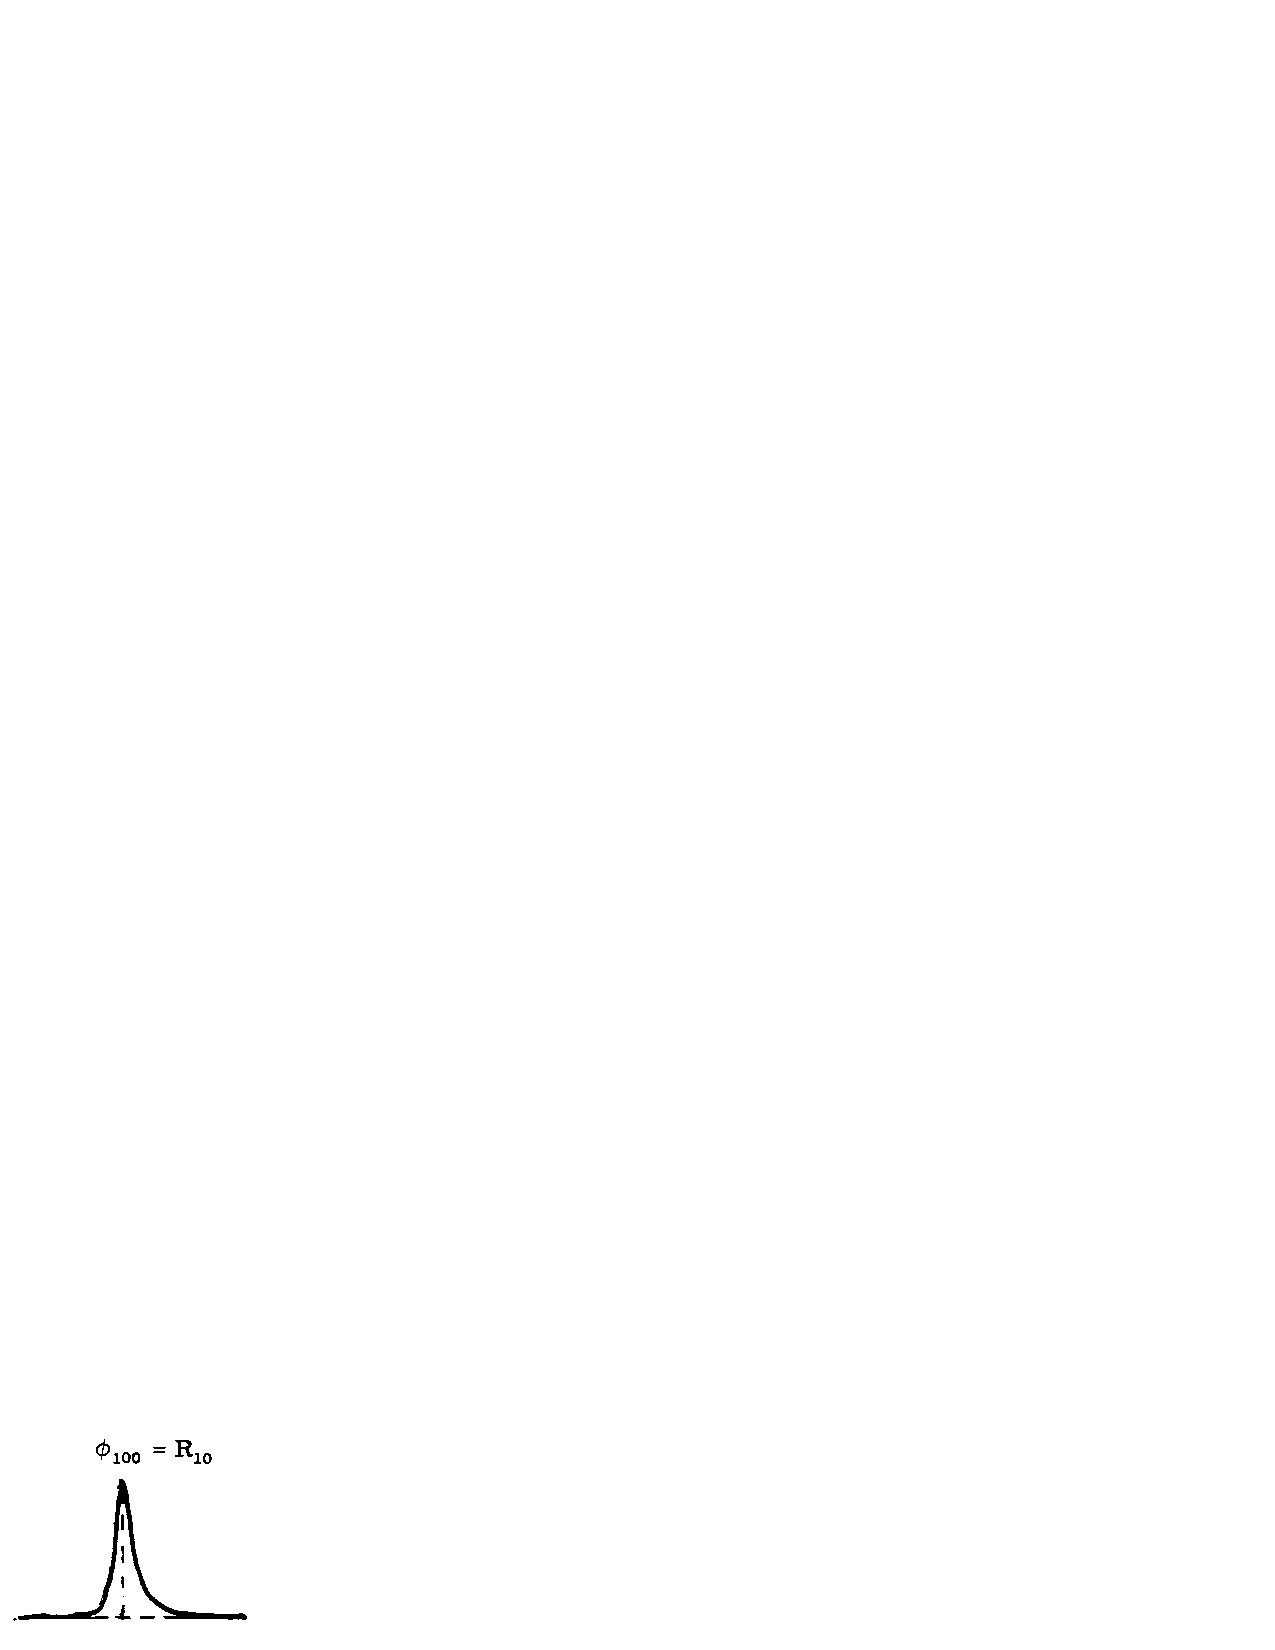
\includegraphics[scale=0.75]{fig5-1a}
\end{center}
\caption{}
\label{fig5-1a}
\end{figure}

\begin{figure}
\begin{center}
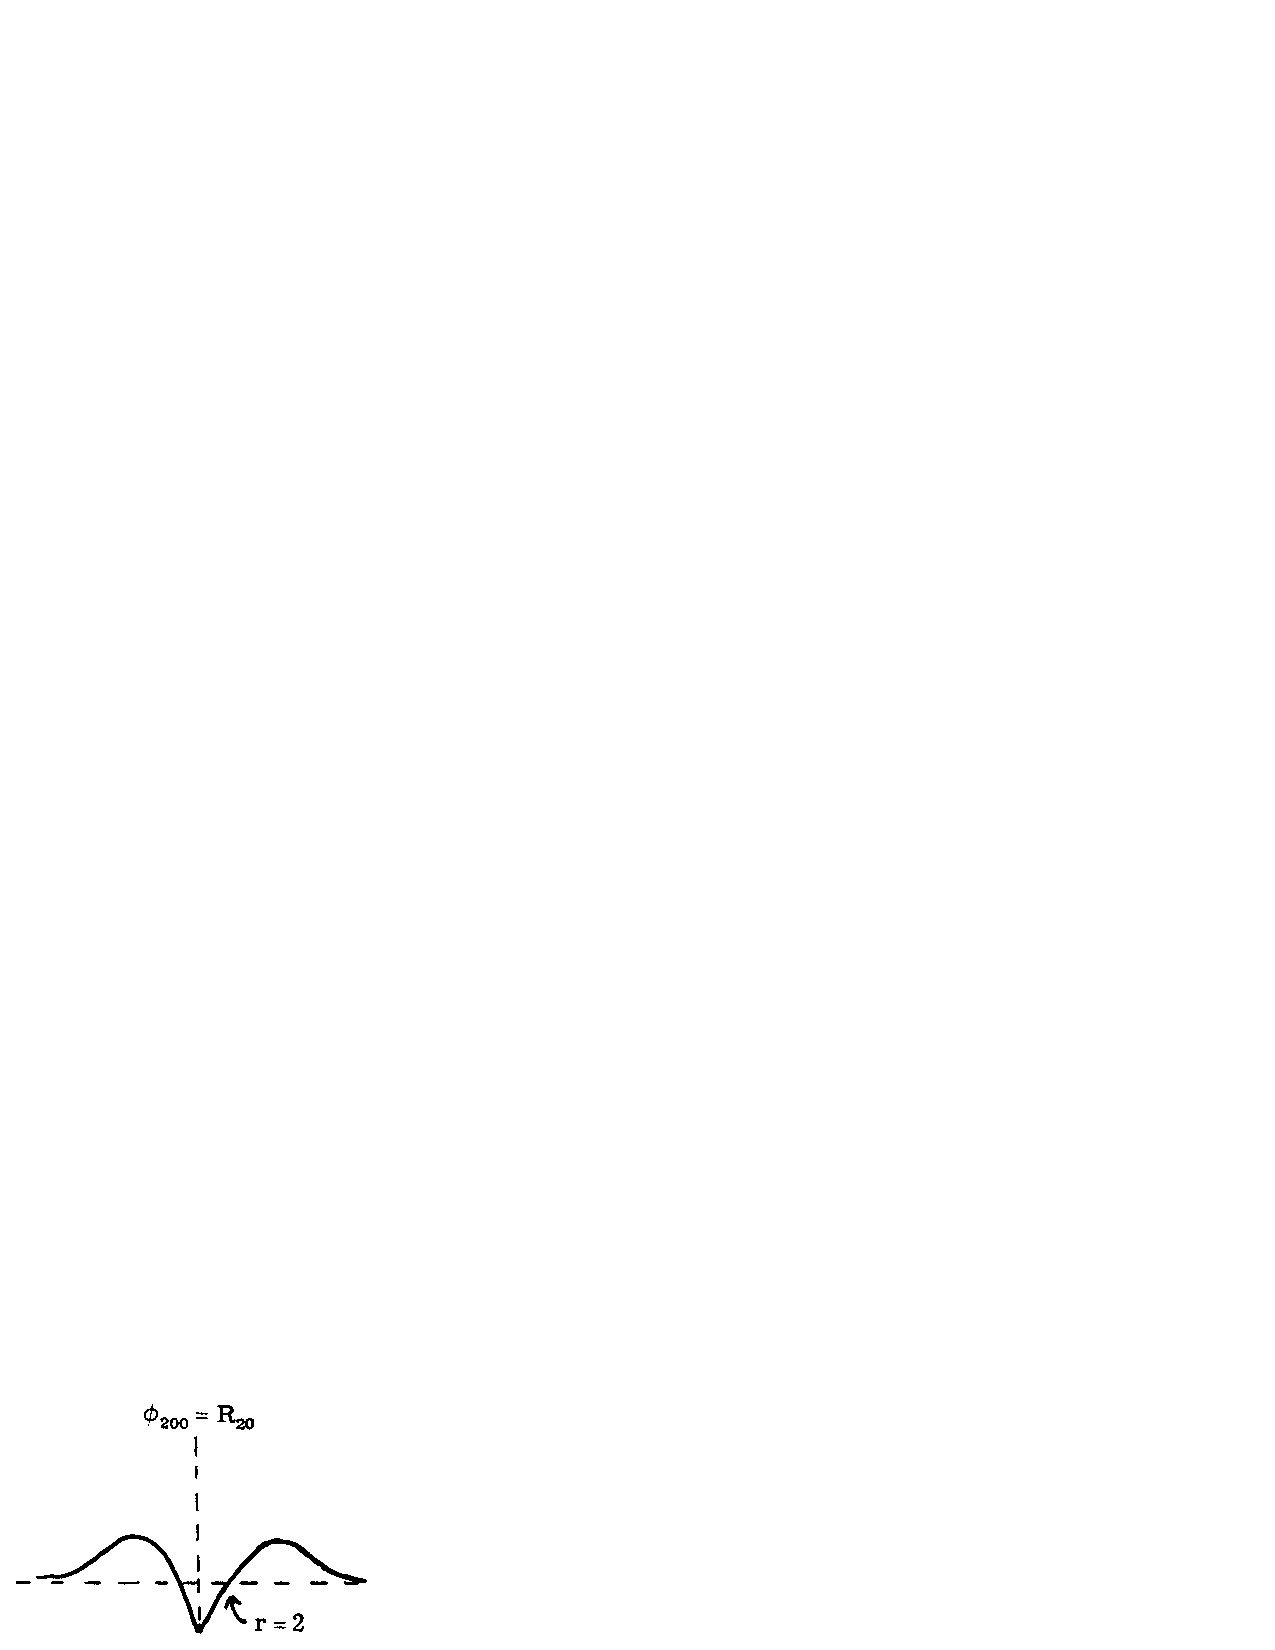
\includegraphics[scale=0.75]{fig5-1b}
\end{center}
\caption{}
\label{fig5-1b}
\end{figure}

\begin{figure}
\begin{center}
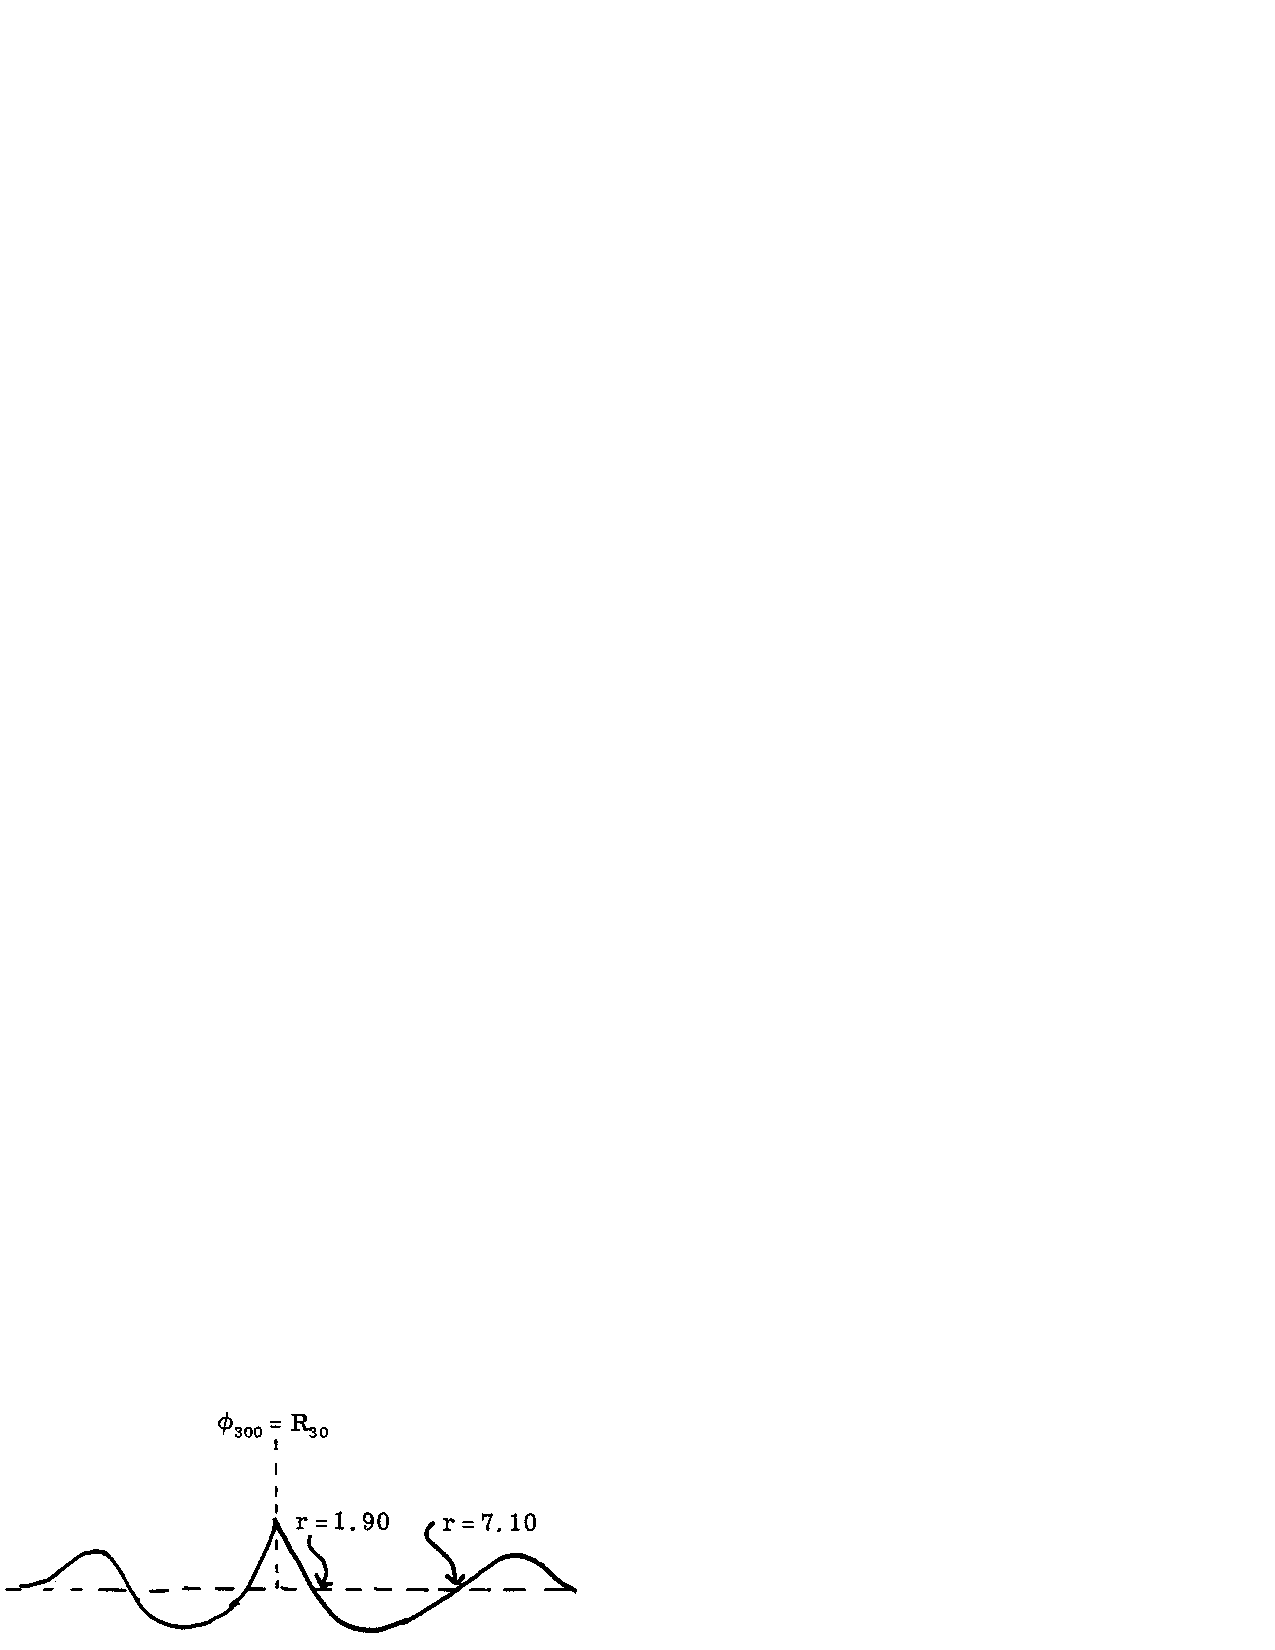
\includegraphics[scale=0.75]{fig5-1c}
\end{center}
\caption{}
\label{fig5-1c}
\end{figure}

The first excited $l = 0$ states, denoted as $R_{20} (r)$, must be
orthogonal to $R_{10} (r)$ and hence, it has the form in Figure
\ref{fig5-1b}.  Forcing a radial node as in Figure \ref{fig5-1c},
necessarily leads to higher gradients, for normalized wavefunctions,
and hence, a higher kinetic energy.
Hence, the optimum $R_{20}(r)$ orbital is much more extended than 
$R_{10}(r)$ in order to decrease the gradients due to the radial node.  Of 
course, expanding the wavefunction increases ${\bar r}$, and hence, makes 
the potential energy less negative.  The final orbital is
\begin{equation}
R_{20} (r) = \left( {1 \over 2} r - 1 \right) e^{-{1 \over 2}r}.
\end{equation}
Higher states have additional nodal planes.

In order to refer quickly to these various solutions, we will
introduce a number $n$, defined to be one greater than the total
number of nodal planes, radial plus angular.  Thus, the ground state
wavefunction (\ref{chap5-eqno5}) is $n = 1$.  The function $R_{20}(r)$
is zero for $r = 2$ independent of $\theta$ and $\varphi$.  Thus, the
wavefunction
\begin{equation}
\phi_{200} \left( r , \theta , \varphi \right) = R_{20} (r) Z_{lm} ( 
\theta , \varphi )
\end{equation}
has one spherical nodal surface, at $r = 2a_0$, and consequently, $n = 
2$.  The next $l = 0$ state is
\begin{equation}
\phi_{300} = R_{30} Z_{00}
\end{equation}
where
\begin{equation}
R_{30}(r) = \left( {2 \over 27} r^2 - {2 \over 3} r+1 \right) e^{-{1 \over 
2}r}
\end{equation}
with radial nodes at $r = 1.902$ and $r = 7.098$, note that the inner node 
lies close to that of $R_{20}$.

\begin{figure}
\begin{center}
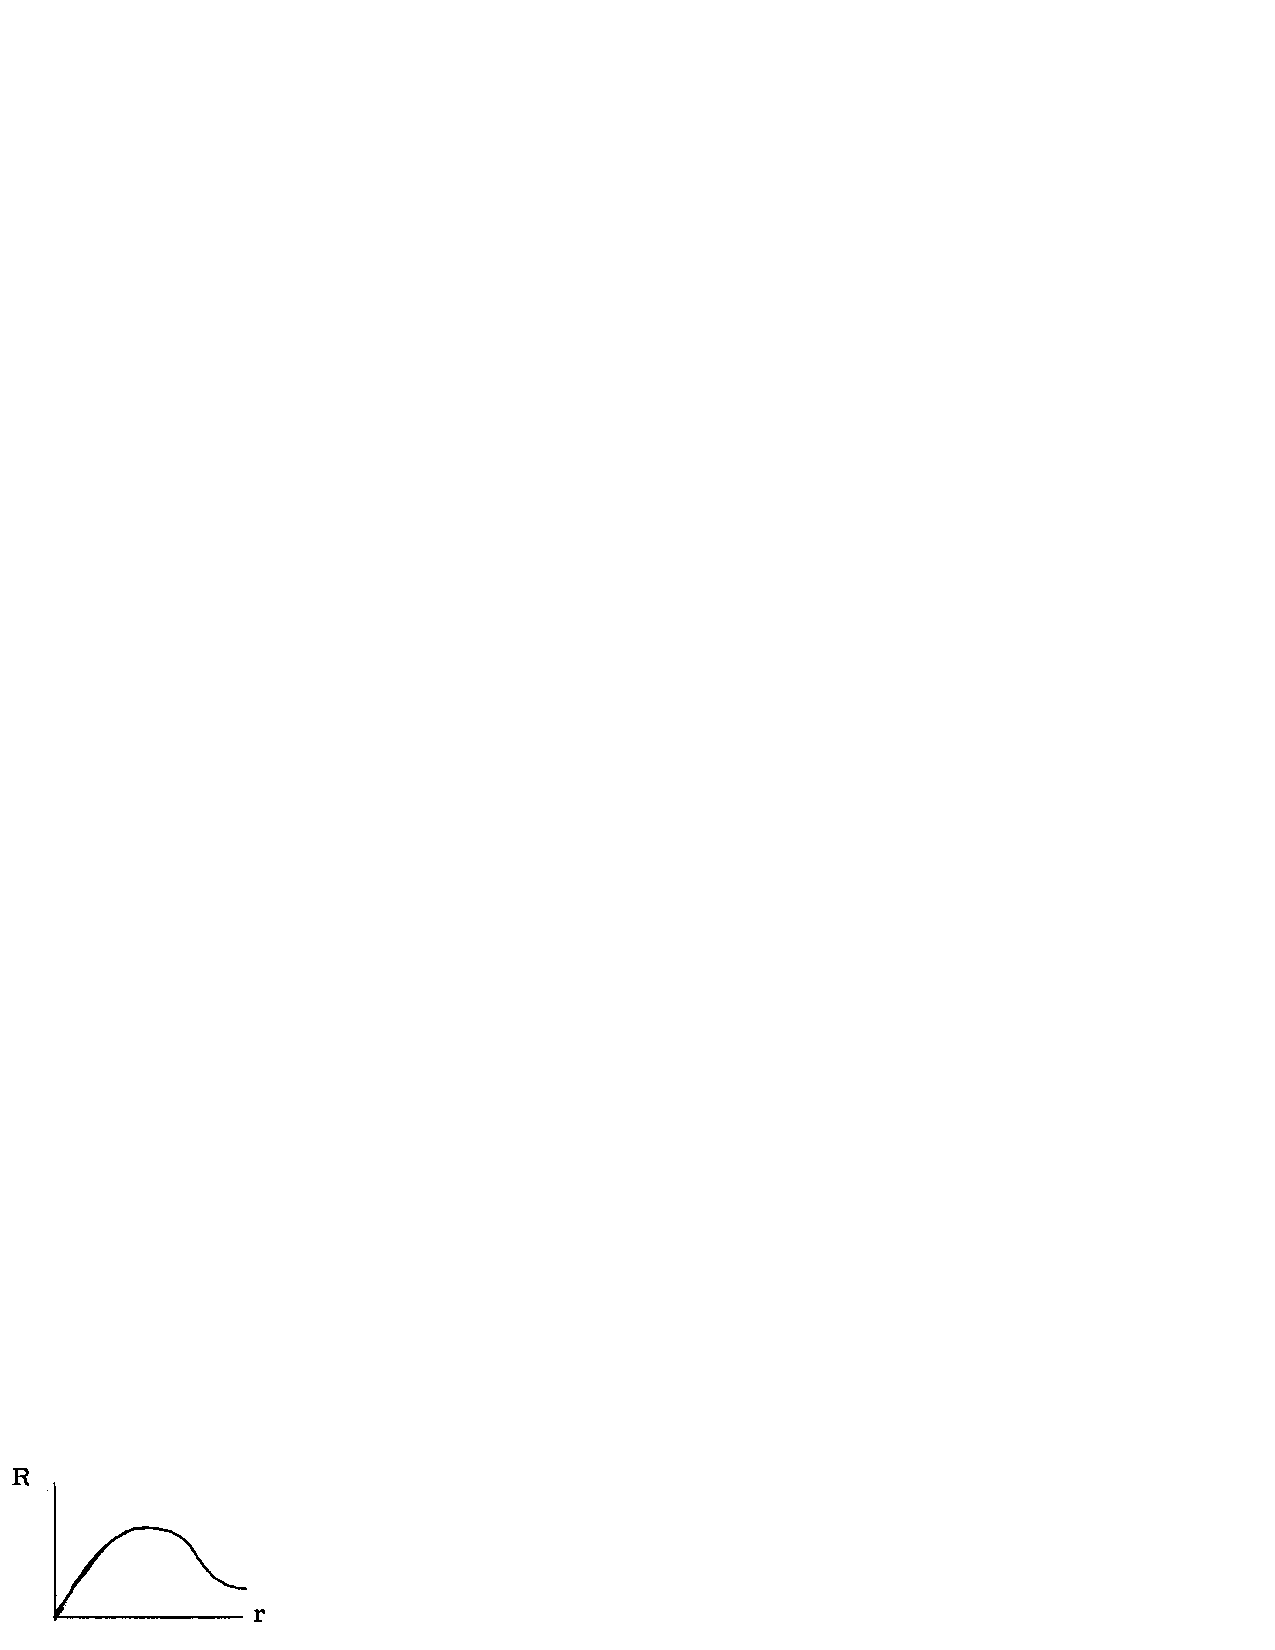
\includegraphics[scale=0.75]{fig5-2a}
\end{center}
\caption{}
\label{fig5-2a}
\end{figure}

\begin{figure}
\begin{center}
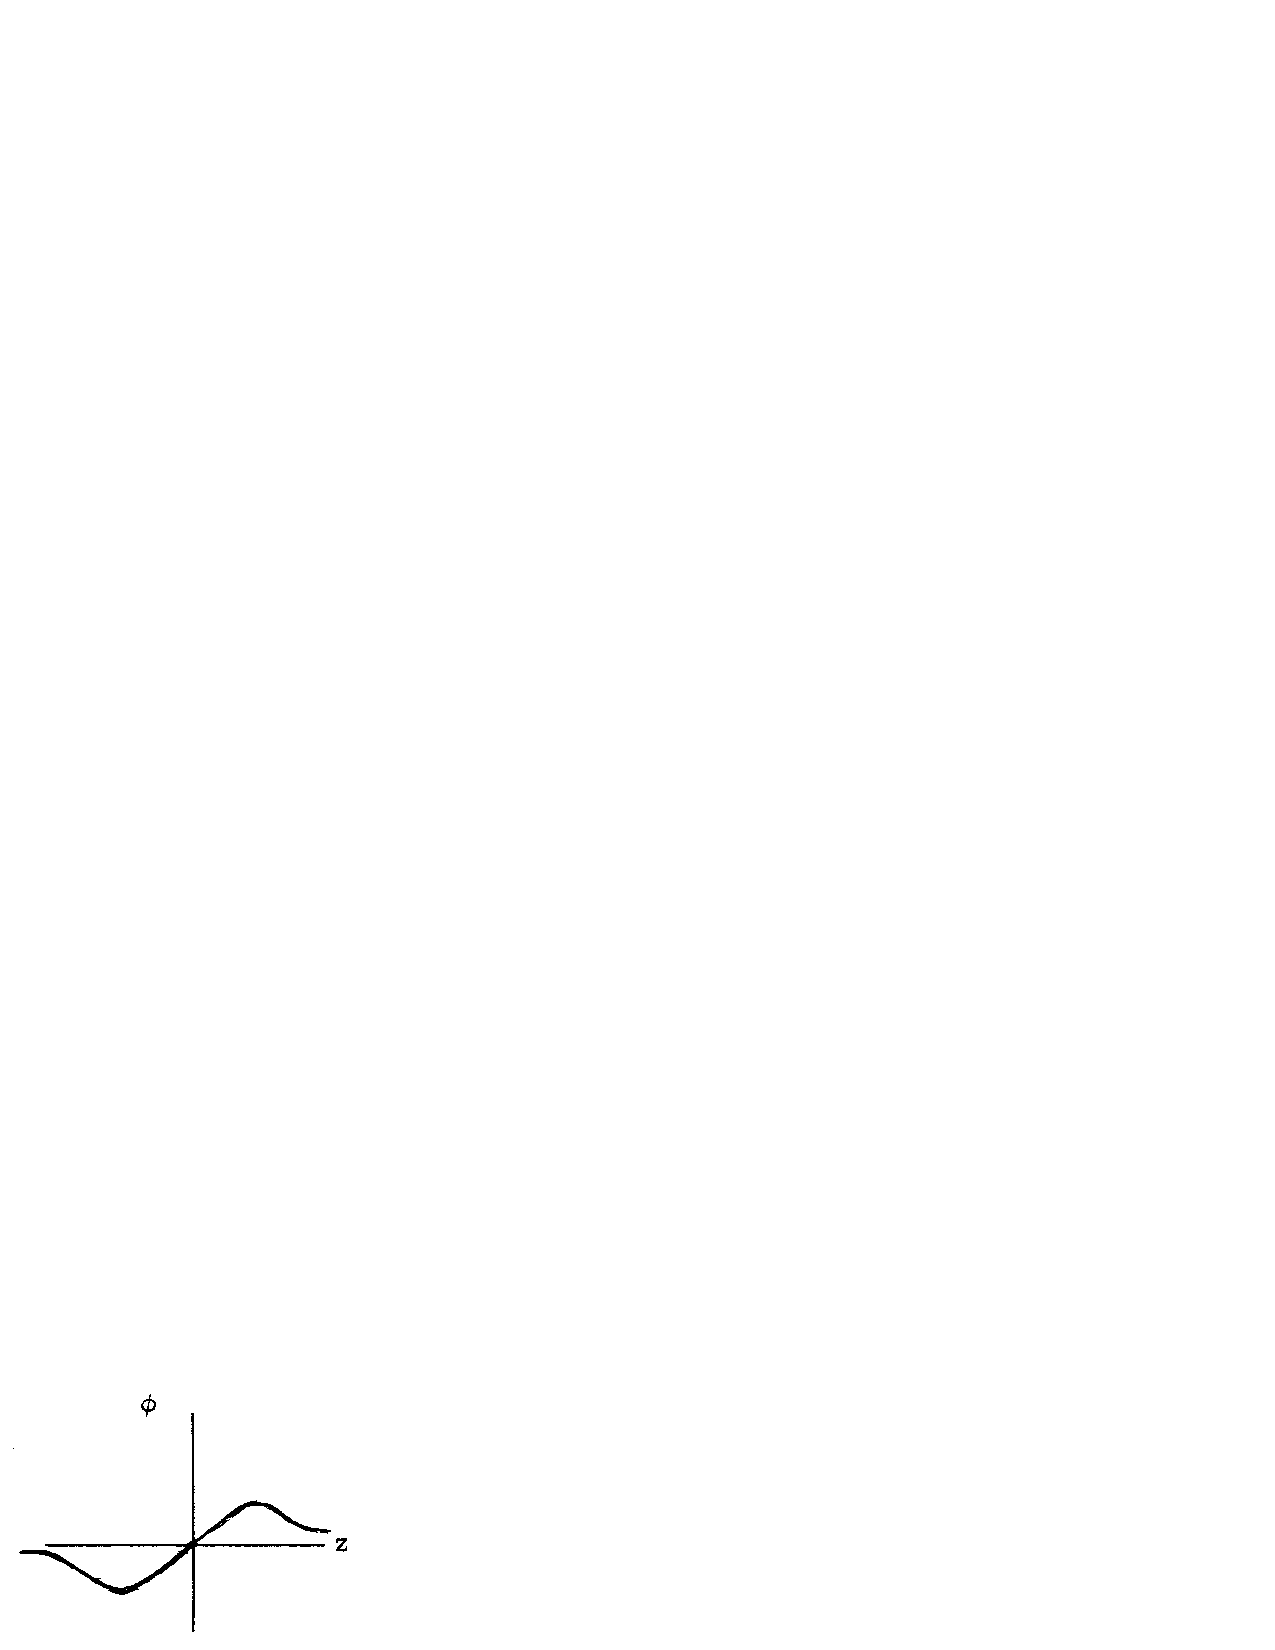
\includegraphics[scale=0.75]{fig5-2b}
\end{center}
\caption{}
\label{fig5-2b}
\end{figure}

Consider now, the functions with $l = 1$ and $m = 0$,
\begin{equation}
\phi ( r , \theta , \varphi ) = R ( r ) Z_{10} ( \theta , \varphi ) = R 
(r) \cos \theta .
\end{equation}
In this case, we must have $R(r) \rightarrow 0$ and $r \rightarrow 0$,
since otherwise $\phi$ would be multi-valued at $r = 0$.  Thus, the
smoothest allowed radial function, i.e., the lowest energy, is of the
form in Figure \ref{fig5-2a}.
Combining this radial form with $\cos \theta$, and plotting along the
Z axis, leads to the form in Figure \ref{fig5-2b}, a function with one
planar nodal surface, the xy plane.  Thus, this state has $n = 2$.
The precise form of the radial function is
\begin{equation}
R_{21} = re^{-{1 \over 2}r}
\end{equation}
and the total wavefunction is
\begin{equation}
\phi_{210} = r \cos \theta e^{-{1 \over 2}r} = ze^{-{1 \over 2}r}.
\end{equation}
Just as for the $R_{20}(r)$ function, the presence of the nodal plane in 
$R_{21}$ leads to an increase in the spatial extent of the wavefunction. 
Since the three $l = 1$ functions are equivalent in shape, differing only 
in the orientation of the nodal plane, the radial function is
independent of $m$.

The radial function for the next higher $l = 1$ states, $n = 3$, must have 
an additional radial nodal plane in order to be orthogonal to $R_{21}$, as 
in Figure \ref{fig5-3a}.  The precise form is
\begin{equation}
R_{31} (r) = r \left( {1 \over 6} r - 1 \right) e^{-{1 \over 3}r}.
\end{equation}
Combining $R_{31}(r)$ with the angular function $Z_{10} (\theta , \varphi)$ 
leads to
\begin{equation}
\phi_{310} ( r , \theta , \varphi ) = z \left( 1 - {1 \over 6} r \right) 
e^{-{1 \over 3}r}.
\end{equation}
Thus, $\phi_{310}$ has two nodal surfaces, one is spherical at $r = 
6a_0$, 
and the other is planar, the xy plane, as illustrated in Figure \ref{fig5-3b}.

\begin{figure}
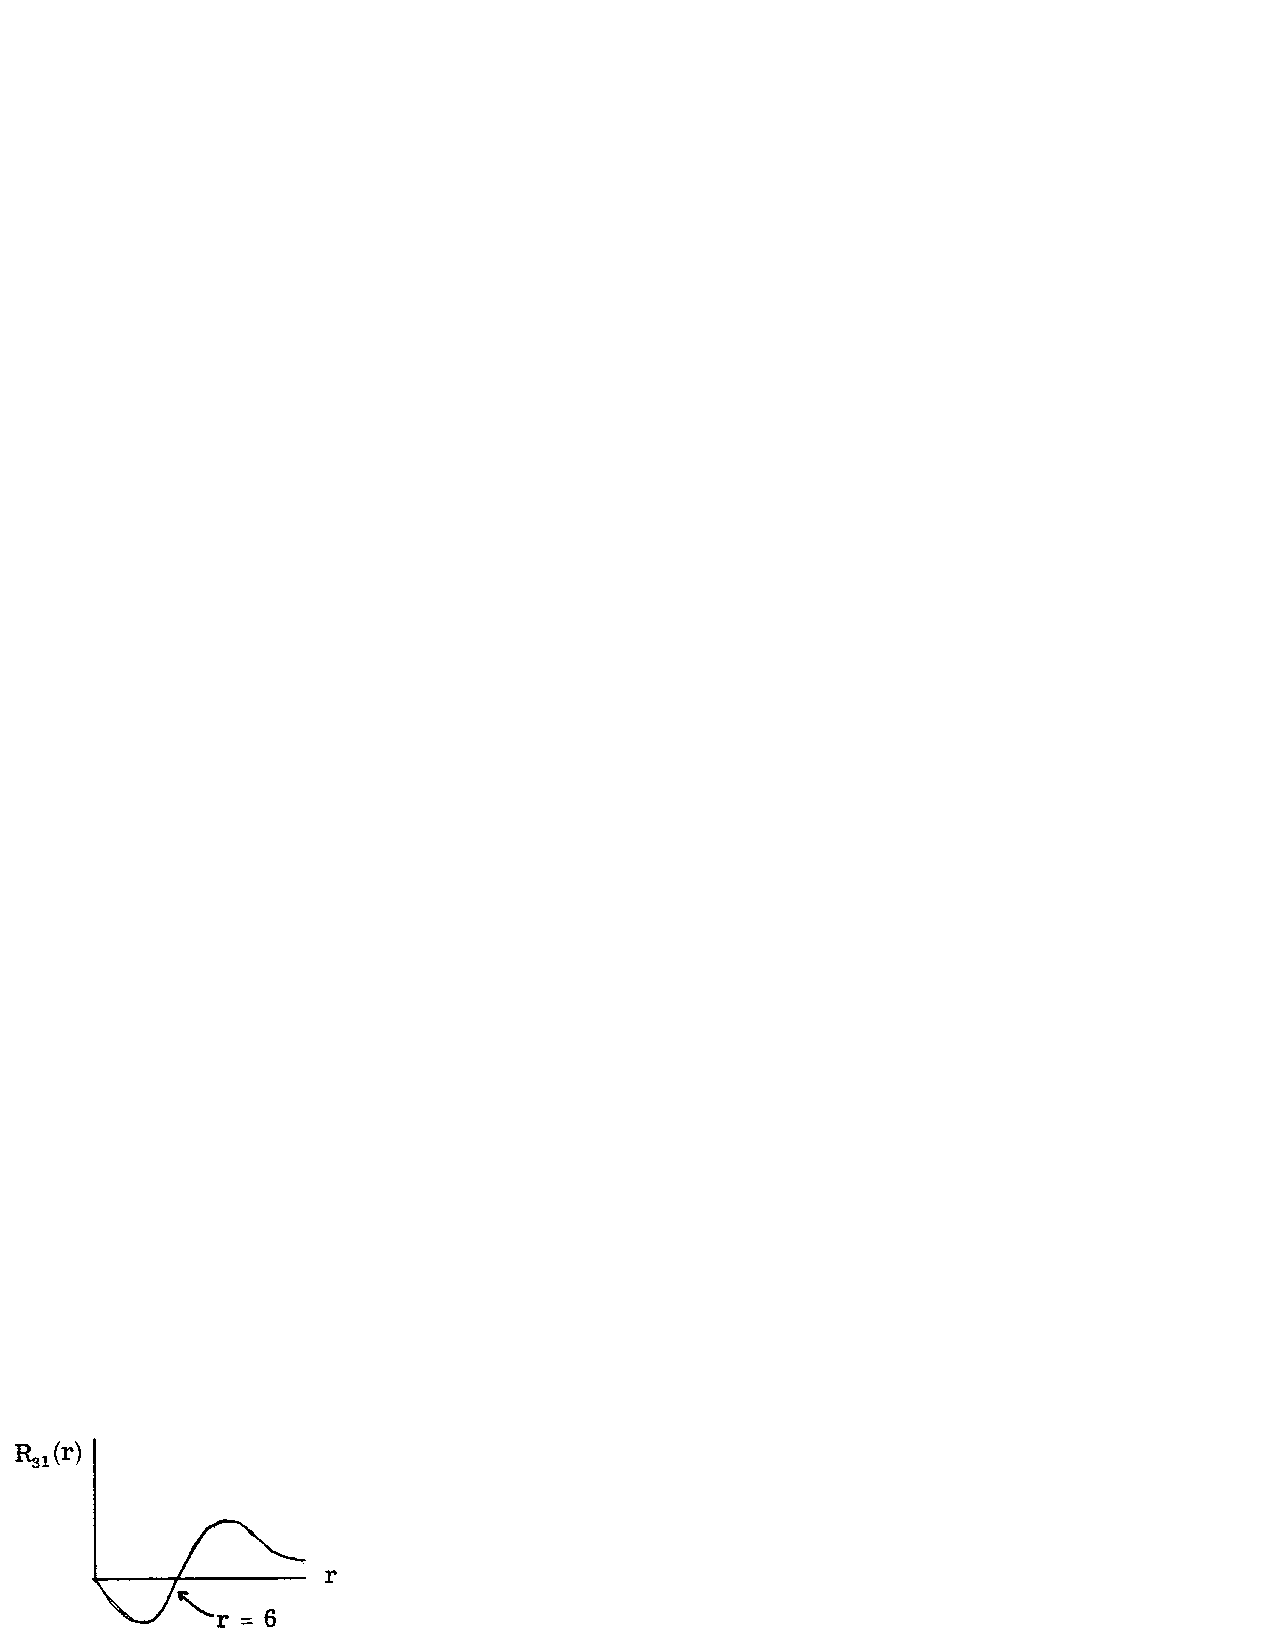
\includegraphics[scale=0.75]{fig5-3a}
\caption{}
\label{fig5-3a}
\end{figure}

\begin{figure}
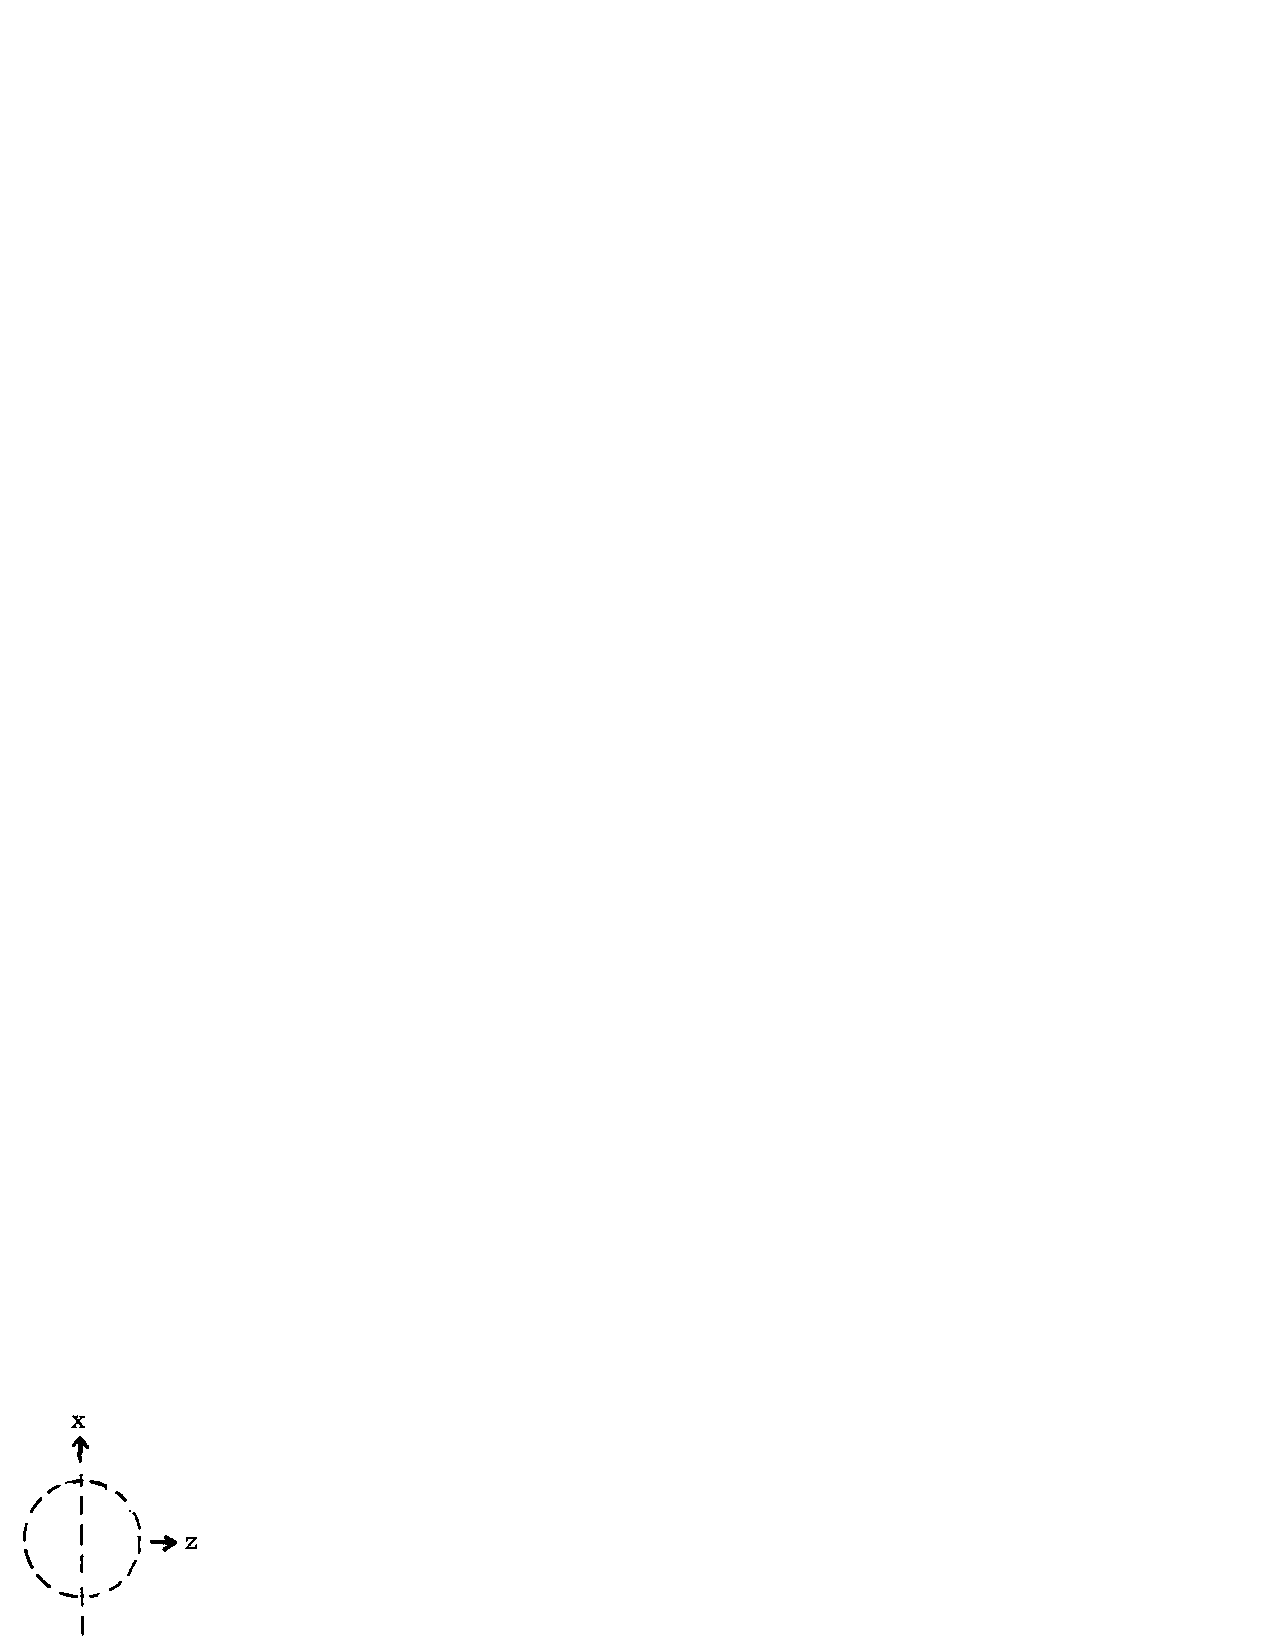
\includegraphics[scale=0.75]{fig5-3b}
\caption{}
\label{fig5-3b}
\end{figure}

For higher angular momenta, $l$, we find that $R_{nl}(r) \rightarrow r^l$ 
as $r \rightarrow 0$, in order that $\phi ( r , \theta , \varphi )$
be single valued at $r = 0$.  The lowest $n$, no radial nodal surfaces, 
is $n = l + 1$, leading to the general form
\begin{equation}
R_{nl} (r) = r^l e^{- {1 \over n}r} ~~~~~~~\left( n = l + 1 \right)
\end{equation}
see the next section for derivation.

The final energy of these states is given by
\begin{equation}
E = - {1 \over 2} {Z^2 \over n^2} .
\end{equation}
Thus, increasing the number of nodal surfaces ($n$) leads to an
increase of the energy (less negative). The unexpected result here is
that the energy is determined only by the total number of nodal
surfaces, independent of whether they are radial or angular. This
result is special to the Coulomb potential $V(r) = - {Z \over r}$.
For a more general potential $V(r)$, the energy depends on $n$ and $l$.

\subsection{Quantitative Aspects of Hydrogen Atom}

Using atomic units, the Hamiltonian for the hydrogen atom becomes
\begin{equation}
H = - {1 \over 2} \nabla^2 - {Z \over r} .
\label{chap5-eqno6}
\end{equation} To solve for the eigenfunctions of (\ref{chap5-eqno6}), it is
convenient to transform to spherical polar coordinates where the
Laplacian becomes
\begin{equation}
\nabla^2 = {\partial^2 \over \partial r^2} + {2 \over r} {\partial \over 
\partial r} - {{\hat l}^2 \over r^2}
\label{chap5-eqno7}
\end{equation}
and
\begin{equation}
{\hat l}^2 = {\hat l}^2_x + {\hat l}^2_y + {\hat l}^2_x
\end{equation}
is the angular momentum operator.  The eigenfunctions of $H$ can 
then be written as
\begin{equation}
H\Psi_{nlm} = E_{nlm} \Psi_{nlm} ,
\end{equation}
where
\begin{equation}
\Psi_{nlm} = R_{nl} (r) Y_{lm} ( \theta ,\varphi )
\label{chap5-eqno8}
\end{equation} 
and $Y_{lm}(\theta , \varphi)$ are the complex spherical harmonic
functions (angular momentum eigenfunctions) shown in Tables
\ref{chap5-table1a}--\ref{chap5-table1b}.  The states given here all
have energies $E < 0$.  For $E \geq 0$ the eigenfunctions of
(\ref{chap5-eqno2}) are not square-integrable, and we will discuss
them no further.  The spherical harmonic functions satisfy
\begin{equation}
{\hat l}^2 Y_{lm} ( \theta , \varphi ) = l ( l + 1 ) Y_{lm} ( \theta 
,\varphi)
\label{chap5-eqno9a}
\end{equation}
\begin{equation}
{\hat l}_z Y_{lm} ( \theta , \varphi ) = mY_{lm} ( \theta , \varphi 
)
\label{chap5-eqno9b}
\end{equation}
and are simple combinations of the real spherical harmonics, $Z_{lm}$.  
The $Z_{lm}$ are eigenfunctions of ${\hat l}^2$ but not of ${\hat l}_z$.  
That is, ${\hat l}_zZ_{lm} \not= mZ_{lm}$, so that the $m$ in $Z_{lm}$ 
is not strictly the angular momentum projection.  The real form is more 
convenient for molecular systems. Although $l$ and $m$ refer to  
the number of angular nodal planes, $l$ is generally referred to as the 
\emph{angular momentum}, and $m$ is referred to as the \emph{angular
momentum projection} (along the z axis).

Using (\ref{chap5-eqno6}), (\ref{chap5-eqno7}), and
(\ref{chap5-eqno8}) in (\ref{chap5-eqno9}), leads to the differential
equation for the radial function, $R(r)$,
\begin{equation}
\left[ - {1 \over 2} \left( {\partial^2 \over \partial r^2} + {2 \over r} 
{\partial \over \partial r} - {l(l+1) \over r^2} \right) - {Z \over r} 
\right] R_{nl} (r) = E_n R_{nl} (r),
\label{chap5-eqno10}
\end{equation}
where the energy is given by
\begin{equation}
E_n = - {Z^2 \over 2n^2}
\end{equation}
Thus, the energy is independent of the angular momentum, $l$.  However, 
only $l \leq n - 1$ are allowed for any given $n$.

In solving (\ref{chap5-eqno10}), it is customary to substitute
\begin{equation}
P_{nl} (r) = r R_{nl} (r)
\end{equation}
so that (\ref{chap5-eqno10}) becomes
\begin{equation}
\left[ - {1 \over 2} {d^2 \over dr^2} + V_l (r) \right] P_{nl} (r) = E_n 
P_{nl} (r)
\label{chap5-eqno11}
\end{equation}
where
\begin{equation}
V_l (r) = {l(l+1) \over 2r^2} - {Z \over r}.
\label{chap5-eqno12}
\end{equation}
This is just the Schr\"odinger equation for a particle moving in a 
one-dimensional potential $V_l(r)$.  The potential depends upon the value 
of the angular momentum, leading to a different sequence (denoted by $n$) 
of solutions for each angular momentum.

The lowest solution for each angular momentum is easy.  It has the form
\begin{equation}
R(r) = r^l e^{- \zeta r}
\end{equation}
or
\begin{equation}
P(r)  = r^{l+1} e^{- \zeta r}
\end{equation}
Substituting into (\ref{chap5-eqno11}), we obtain
\begin{equation}
\left\{ {(l+1)l \over 2r^2} + \zeta {(l+1) \over r} - {1 \over 2} 
\zeta^2 + {l(l+1) \over 2r^2} - {Z \over r} - E \right\} P_{nl}(r) = 0
\end{equation}
and hence,
\begin{equation}
E = - {1 \over 2} \zeta^2
\label{chap5-eqno13a}
\end{equation}
where
\begin{equation}
\zeta = {Z \over n}
\label{chap5-eqno13b}
\end{equation}
and $n = l + 1$.  Substituting (\ref{chap5-eqno13b}) into
(\ref{chap5-eqno13a}) leads, then, to the total energy
\begin{equation}
E_n = - {Z^2 \over 2n^2}.
\end{equation}

Higher energy solutions are obtained corresponding to each larger
value of $n$.  The other solutions of (\ref{chap5-eqno10}) are listed
in Tables \ref{chap5-table2}--\ref{chap5-table3}, using the real form
of the angular functions, and plotted in Figures \ref{fig5-4} and
\ref{fig5-5}, for the $n = 1 , 2 , 3 ,$ and $n = 4$ states,
respectively.

\begin{figure}
\includegraphics[scale=0.75]{fig5-4}
\caption{Contour plots of selected $n = 1,
2$, and 3 atomic orbitals, $Z = 1$, i.e., for the hydrogen atom.  Long
dashed lines indicate nodal planes; solid lines indicate positive
contours, and short dashed lines indicate negative contours. The most
diffuse contour is .0025 atomic unit.  Each successive contour is a
factor of 2 larger.  The contours plotted are 0.0025, 0.0050, 0.0100,
0.0200, 0.0400, etc.  All quantities are in atomic units.}
\label{fig5-4}
\end{figure}

\begin{figure}
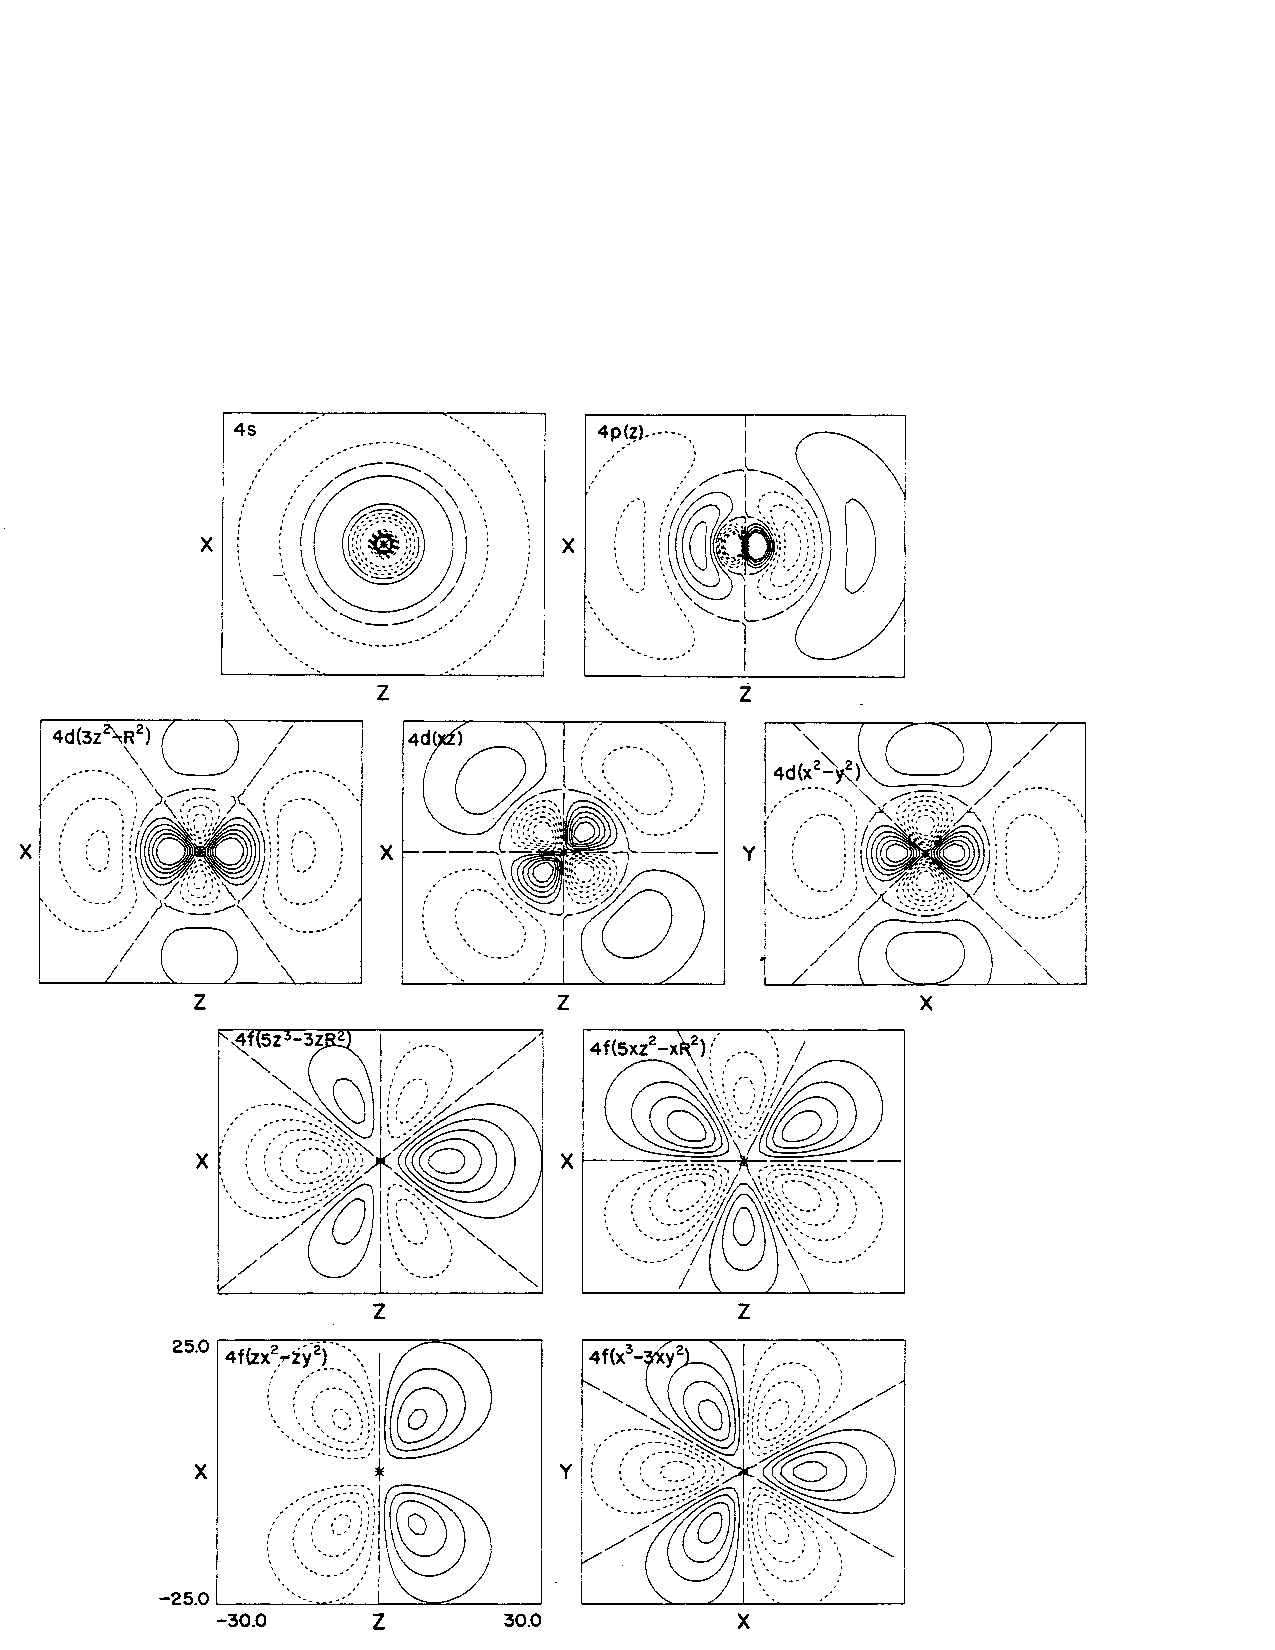
\includegraphics[scale=0.75]{fig5-5}
\caption{Contour plots for selected $n = 4$ orbitals, $Z = 
1$.  Contour conventions, as in Figure 1.  However, the contour values
are .0025, .0050, .0075, .0100, and .0125.}
\label{fig5-5}
\end{figure}

For each $n$ there are solutions corresponding to $l = 0 , 1 , ... , n - 
1$.  The eigenfunction of the H atom are shown in Table
\ref{chap5-tableaa}.

\begin{table}
\caption{}
\label{chap5-tableaa}
\begin{tabular}{ccc}\\ \hline
$n$ & $l$ & notation\cr
1 & 0 & $1s$\cr
2 & 0 & $2s$\cr
2 & 1 & $2p$\cr
3 & 0 & $3s$\cr
3 & 1 & $3p$\cr 
3 & 2 & $3d$\cr
\hline
\end{tabular}\\
where s, p, d, f, g, etc., denote $l =$ 1, 2, 3, 4, etc.
\end{table}

\begin{table}
\caption{The radial functions, in atomic units, for the 
hydrogen-like atoms.  The sign convention used here is that 
$R_{nl}(r) > 0$ for large $r$, a more common convention is 
$R_{nl}(r) > 0$, as $r \rightarrow 0$.  This is convenient for 
considerations of interactions of orbitals of different atoms of a 
molecule.}
\label{chap5-table2}
\begin{tabular}{ccc} \\ \hline
$(nl)$ & Spectroscopic & $R_{nl}(r)$\cr 
(10) & 1s & $2Z^{{3 \over 2}}e^{-Zr}$\cr
(20) & 2s & ${1 \over \sqrt{2}} Z^{{3 \over 2}} \left(-1 + {Z \over 2} 
r \right) e^{-{Z \over 2}r}$\cr
(21) & 2p & ${1 \over 2 \sqrt{6}} Z^{{5 \over 2}} re^{-{Z \over 
2}r}$\cr
(30) & 3s & ${2 \over 3\sqrt{3}} Z^{{3 \over 2}} \left(1-{2 \over 
3}Zr + {2 \over 27} z^2r^2\right)e^{-{Z \over 3}r}$\cr
(31) & 3p & ${8 \over 27\sqrt{6}} Z^{{5 \over 2}}r\left(-1+{Zr \over 
6} \right) e^{-{Z \over 3}r}$\cr
(32) & 3d & ${4 \over 81\sqrt{30}} Z^{{7 \over 2}} r^2 e^{-{Z \over 
3}r}$\cr
(40) & 4s & ${1 \over 4} Z^{{3 \over 2}} \left( -1 + {3 \over 4} Zr - 
{1 \over 8} Z^2 r^2 + {1 \over 192} Z^3 r^3 \right) e^{-{Z \over 
4}r}$\cr
(41) & 4p & ${10 \over 32\sqrt{15}} Z^{{5 \over 2}} \left( 1 - {1 
\over 4} Zr + {1 \over 80} Z^2 r^2 \right) re^{-{Z \over 4}r}$\cr
(42) & 4d & ${1 \over 64\sqrt{5}} Z^{{7 \over 2}} \left(-1 + {1 \over 
12} Zr \right) r^2 e^{-{Z \over 4}r}$\cr
(43) & 4f & ${1 \over 768\sqrt{35}} Z^{{9 \over 2}} r^3e^{-{Z \over 
4}r}$\cr
\hline
\end{tabular}
\end{table}

\begin{table}
\caption{Wavefunctions for the hydrogen-like atoms, 
through $n = 3$, in real form.  In atomic units.}
\label{chap5-table3}
\begin{tabular}{cc} \\ \hline
State & Wavefunction\cr
1s & $\left({Z^3 \over \pi} \right)^{{1 \over 2}} e^{-Zr}$\cr
2s & $\left({Z^3 \over 8 \pi} \right)^{{1 \over 2}} \left(1- {1 \over 
2} r \right) e^{-{1 \over 2}Zr}$\cr
2p$_{x,y,z}$ & $\left({Z^5 \over 32 \pi} \right)^{{1 \over 2}} 
\left\{\matrix{x\cr y\cr z\cr}\right\} e^{-{1 \over 2}Zr}$\cr
3s & $\left({Z^3 \over 27 \pi} \right)^{{1 \over 2}} \left( 1 - {2 
\over 3} Zr + {2 \over 27} Z^2 r^2 \right) e^{-{1 \over 3}Zr}$\cr
3p$_{x,y,z}$ & $\left( {8Z^5 \over 729\pi} \right)^{{1 \over 2}} 
\left(1 - {1 \over 6} Zr \right) \left\{\matrix{x\cr y\cr 
z\cr}\right\}e^{-{1 \over 3}Zr}$\cr
3d$_{z^2,xz,yz,x^2-y^2,xy}$ & ${1 \over 81}\left({Z^7 \over \pi} 
\right)^{{1 \over 2}} \left\{\matrix{6^{-{1 \over 2}}(3z^2-r^2)\cr
y^{{1 \over 2}}xz\cr
2^{{1 \over 2}}(x^2-y^2)\cr
2^{-{1 \over 2}}xy\cr}\right\}e^{1{1 \over 3}Zr}$\cr
\end{tabular}
\end{table}

Throughout this course, orbitals will be represented by \emph{contour
plots}, such as in Figures \ref{fig5-4} and \ref{fig5-5}, and hence,
you should be sure to learn how to interpret them.  In Figure
\ref{fig5-4}, all but one plot is in the plane passing through the
origin and lying in the $xz$ plane, the exception is in the $xy$
plane.  Each contour line corresponds to a particular amplitude for
this plane.  The lines with long dashes, indicate zero amplitude while
solid and dotted lines indicate positive and negative amplitude,
respectively.  When comparing a bunch of orbitals, as in Figures
\ref{fig5-4} and \ref{fig5-5}, we will generally use the same scale
and will always use the same amplitudes for all plots.

Two standard conventions are used for spacing the amplitudes being 
plotted.  Our normal convention involves use of a constant increment in 
contour amplitudes.  Thus, in Figure \ref{fig5-5}, contours corresponding to 
$\pm$0.0125, $\pm$0.0075, $\pm$0.0050, $\pm$0.0025, 0.00 are plotted. This 
is appropriate when all orbitals being shown have similar sizes, in Figure 
\ref{fig5-5} all orbitals correspond to $n = 4$, and hence,
are of nearly the same size. The other convention, referred to as a
log plot, involves a constant factor in space the contours.  Thus, in
Figure \ref{fig5-4}, the contours corresponding to 0.0, 0.0025,
0.0050, 0.0100, 0.0200, 0.0400, etc., are plotted.  This is
appropriate for showing orbitals of widely disparate sizes, as in
Figure \ref{fig5-4} where $n = 1$, $n = 2$, and $n = 3$ orbitals are
shown.

For the $1s$ and $2p$ orbitals, each contour amplitude occurs once and
interpretation is straightforward.  For the $2s$, and certain other
orbitals, interpretation is a little more difficult since there are
maxima with $r \not= 0$, as illustrated in Figure \ref{fig5-6}.  In
this case, the presence and position of the maximum is not obvious
without careful examination of the positions of the nodal lines, e.g.,
examine the 4s orbital in Figure 5.
\begin{figure}
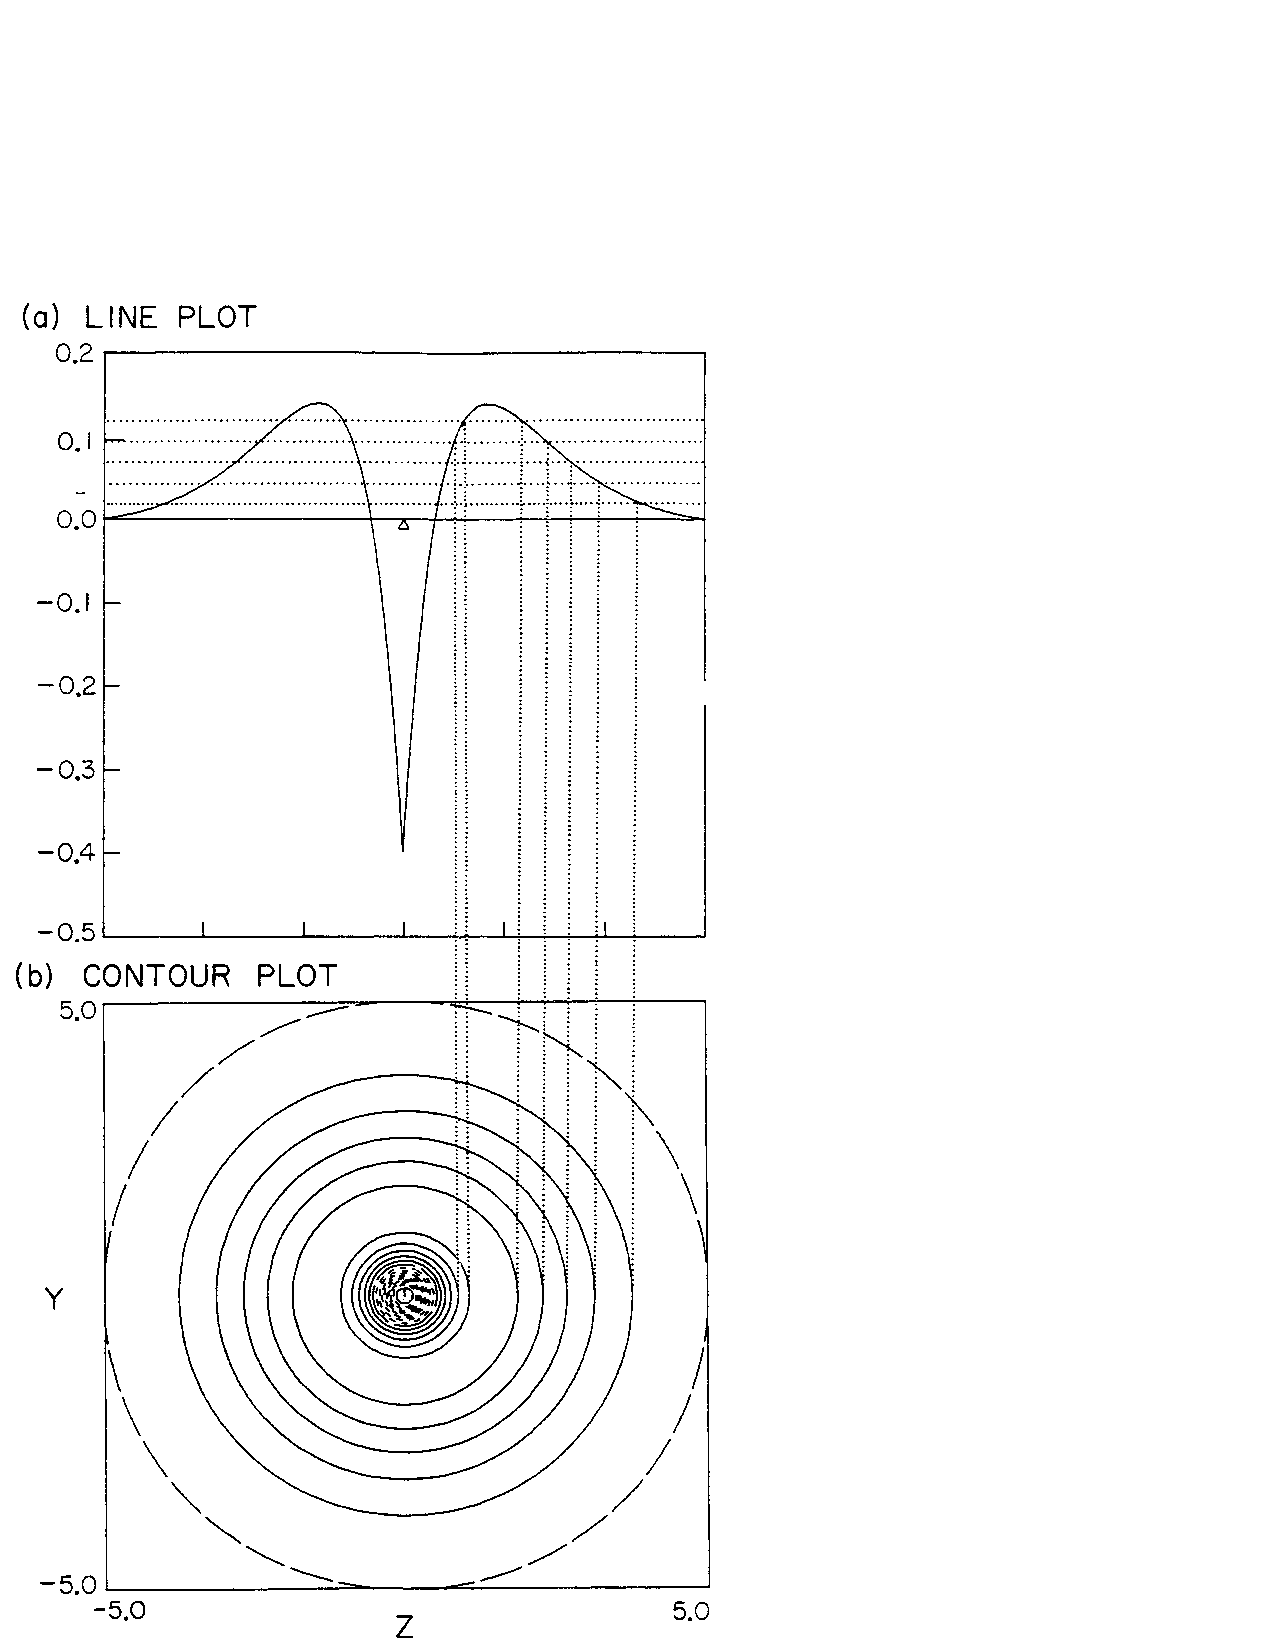
\includegraphics[scale=0.75]{fig5-6}
\caption{Comparison of line
and contour plots for a 2s-like orbital (the orbital plotted is not a
2s orbital, but has been modified to go to zero at $r = 5a_0$).  Note
that with the contour plot, the maximum is indicated by a wide space
between positive contours.}
\label{fig5-6}
\end{figure}

\subsection{Sizes of the Orbitals}

The bound eigenstates of a particle moving in a Coulomb potential
\begin{equation}
V(r) = - {Z \over r},
\end{equation}
lead to total kinetic and potential energies, $T$ and $V$, that are related 
by $2T = - V$.  Since the total energy is $E = T + V$, we have $E = - T$ 
and $E = 1/2V$.  This result is called the \emph{virial theorem}. Since
\begin{equation}
E = - {Z^2 \over 2n^2} ,
\end{equation}
we find that
\begin{equation}
T = {Z^2 \over n^2}
\label{chap5-eqno14}
\end{equation}
and
\begin{equation}
V = - {Z^2 \over n^2}.
\end{equation}
    
Since the potential energy of a particle in state $\phi$ is given by
\begin{equation}
V = \langle \phi | - {Z \over r} | \phi \rangle ,
\end{equation}
we will define the average distance of the electron from the nucleus, 
${\bar r}$, as
\begin{equation}
V = - {Z \over r} .
\end{equation}
Thus, ${\bar r}$ is the radius for a classical particle to have the same 
potential energy.  This definition leads to
\begin{equation}
{1 \over {\bar r}} = \langle \phi | {1 \over r} | \phi \rangle ,
\end{equation}
and hence, from (\ref{chap5-eqno14}) we obtain
\begin{equation}
{\bar r} = {n^2 \over Z} .
\end{equation}
Thus, for the hydrogen atom, the average radial distance ${\bar r}$ for 
the $n = 1 , 2, 3 , 4$, states are ${\bar r} = 1a_0 = 0.53$\AA, $4a_0 = 
2.1$\AA, $9a_0 = 4.7$\AA, and $16a_0 = 8.5$\AA,
respectively.  Since the bond length of the H$_2$ molecules is $1.4a_0 = 
0.75$\AA, and a typical CH bond length is $2.1a_0 = 1.0$\AA, we see that 
even the $n = 2$ excited H orbitals are much larger than a bond, and the $n = 
3$ excited orbitals are very large indeed.  Considering a fixed $n$, say $n = 
1$, and varying nuclear charge $Z$, we see that the large
atoms have much smaller orbitals, with the average radius of the ls orbital 
of C$^{5+}$ being one-sixth that of hydrogen.

With the definition of size used above, the states of various $l$, 
but the same $n$, have the same size.  Other definitions of size, say
\begin{equation}
{\bar r} = \langle \phi | r | \phi \rangle
\end{equation}
or
\begin{equation}
{\bar r} = \sqrt{\langle \phi | r^2 | \phi \rangle},
\end{equation}
lead to slightly different ${\bar r}$ for different $l$ with the same $n$.  
However, all such definitions lead to overall sizes comparable to
(\ref{chap5-eqno12}). 

In Figure \ref{fig5-7}(a), we present line plots of the $1s$, $2s$ and
$3s$ orbitals of hydrogen, but with the sign changes for $2s$.  These
orbitals are not normalized, rather the amplitude at the nucleus was
taken to be the same value for each orbital. Note that in the region
near the nucleus, $r < la_0$, the $\psi_{2s}$ and $\phi_{3s}$ orbitals
are very similar to $\phi_{1s}$.  For $r < 4a_0$, the outer maximum in
$\psi_{2s}$, the $\psi_{3s}$ orbital is very similar to $\psi_{2s}$.
These observations are general and result from the orthogonality
conditions on the higher energy orbitals.

\begin{figure}
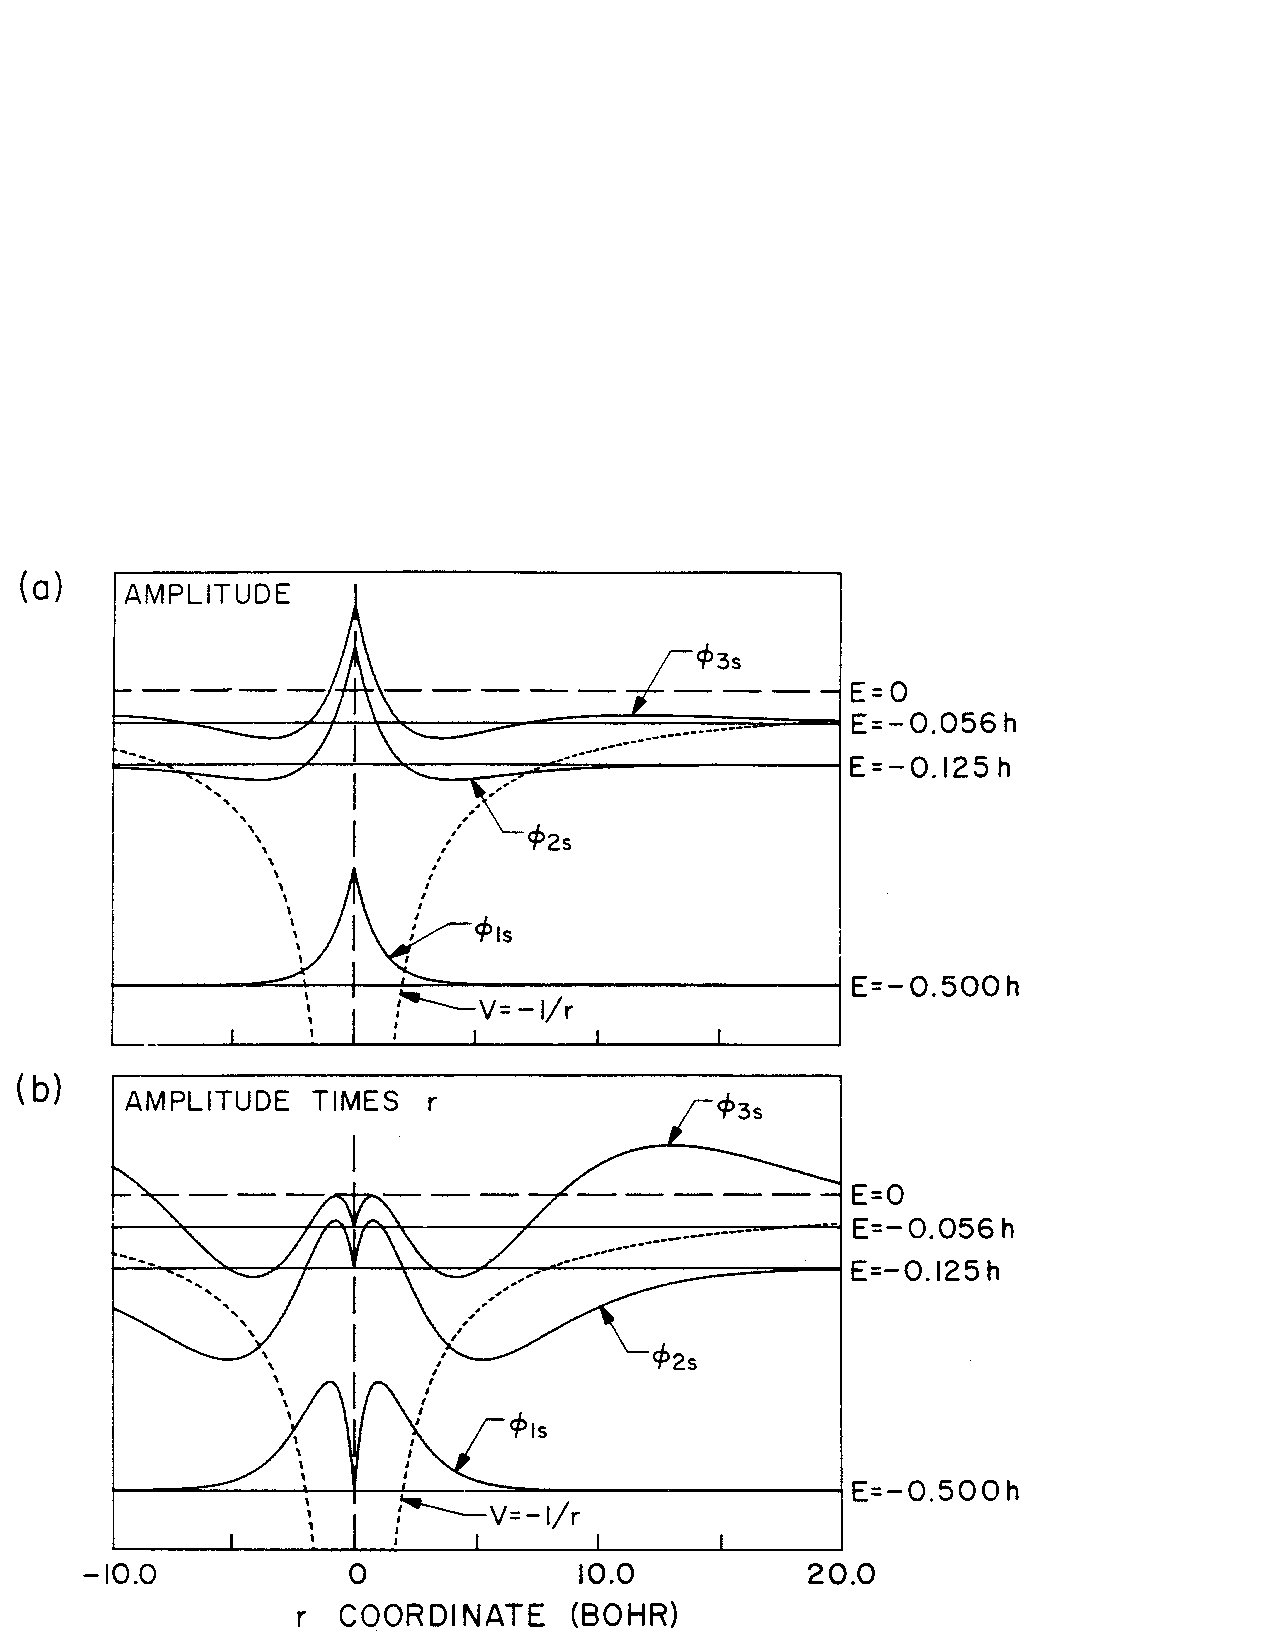
\includegraphics[scale=0.75]{fig5-7}
\caption{(a) The amplitudes of the 1s, 2s, and 3s orbitals of
hydrogen (sign changed for 2s).  Also included is a plot of
the potential energy, $V = - 1/r$ (dotted line).  The line with the
long dashes is the zero of energy for the potential.  For each state,
a solid horizontal line is drawn at the energy for the orbital.  The
orbital is then plotted with this line as the origin.  The orbitals
are not normalized.  (b) The $r \phi$ for the 1s, 2s, and 3s
levels.  Since $(r \phi)^2$ is the probability density for an electron
at distance $r$ from the nucleus, the figure provides the relative
amplitude of being at various $r$.}
\label{fig5-7}
\end{figure}

From Figure \ref{fig5-3a} it would appear that the $\psi_{2s}$ and
$\psi_{3s}$ orbitals are concentrated mainly in the same region as
$\phi_{1s}$. However, in spherical coordinates, the volume element for
the radial integration is $d \tau = r^2 dr$, and hence, the
probability density for the electron to be a distance $r$ from the
nucleus is
\begin{equation}
r^2 \phi^2 ( r ) = [ r \phi ( r ) ]^2 .
\end{equation}
The quantity $r \phi (r)$ is plotted in Figure \ref{fig5-7}(b), where
we see that the probability density is a maximum at $r = 1a_0$ for the
$1s$ orbital, $r = 5a_0$ for the $2s$ orbital, and $r = 13a_0$ for the
$3s$ orbital.

Given an energy
\begin{equation}
E_n = - {1 \over 2n^2} ,
\end{equation}
the classical motion of an electron about a nucleus of charge 1, would be
confined within the radius
\begin{equation}
r_{cl} = {1 \over n^2} = 2 {\bar r} .
\end{equation}
From Figure \ref{fig5-7}(b), we see that the maximum probability
amplitude always occurs within this classically allowed region.
However, there are quite significant amplitudes in the classically
forbidden region.

From (\ref{chap5-eqno12}) we see that if $l \not= 0$, the potential
becomes positively infinite for $r = 0$.  As a result, the
wavefunctions for $l \not= 0$ must go to zero for $r = 0$.  The
potentials (\ref{chap5-eqno12}) for $l = 0$, 1, and 2 are shown in
Figure \ref{fig5-8} along with the amplitudes of the $1s$, $2p$, and
$3s$ orbitals.

\begin{figure}
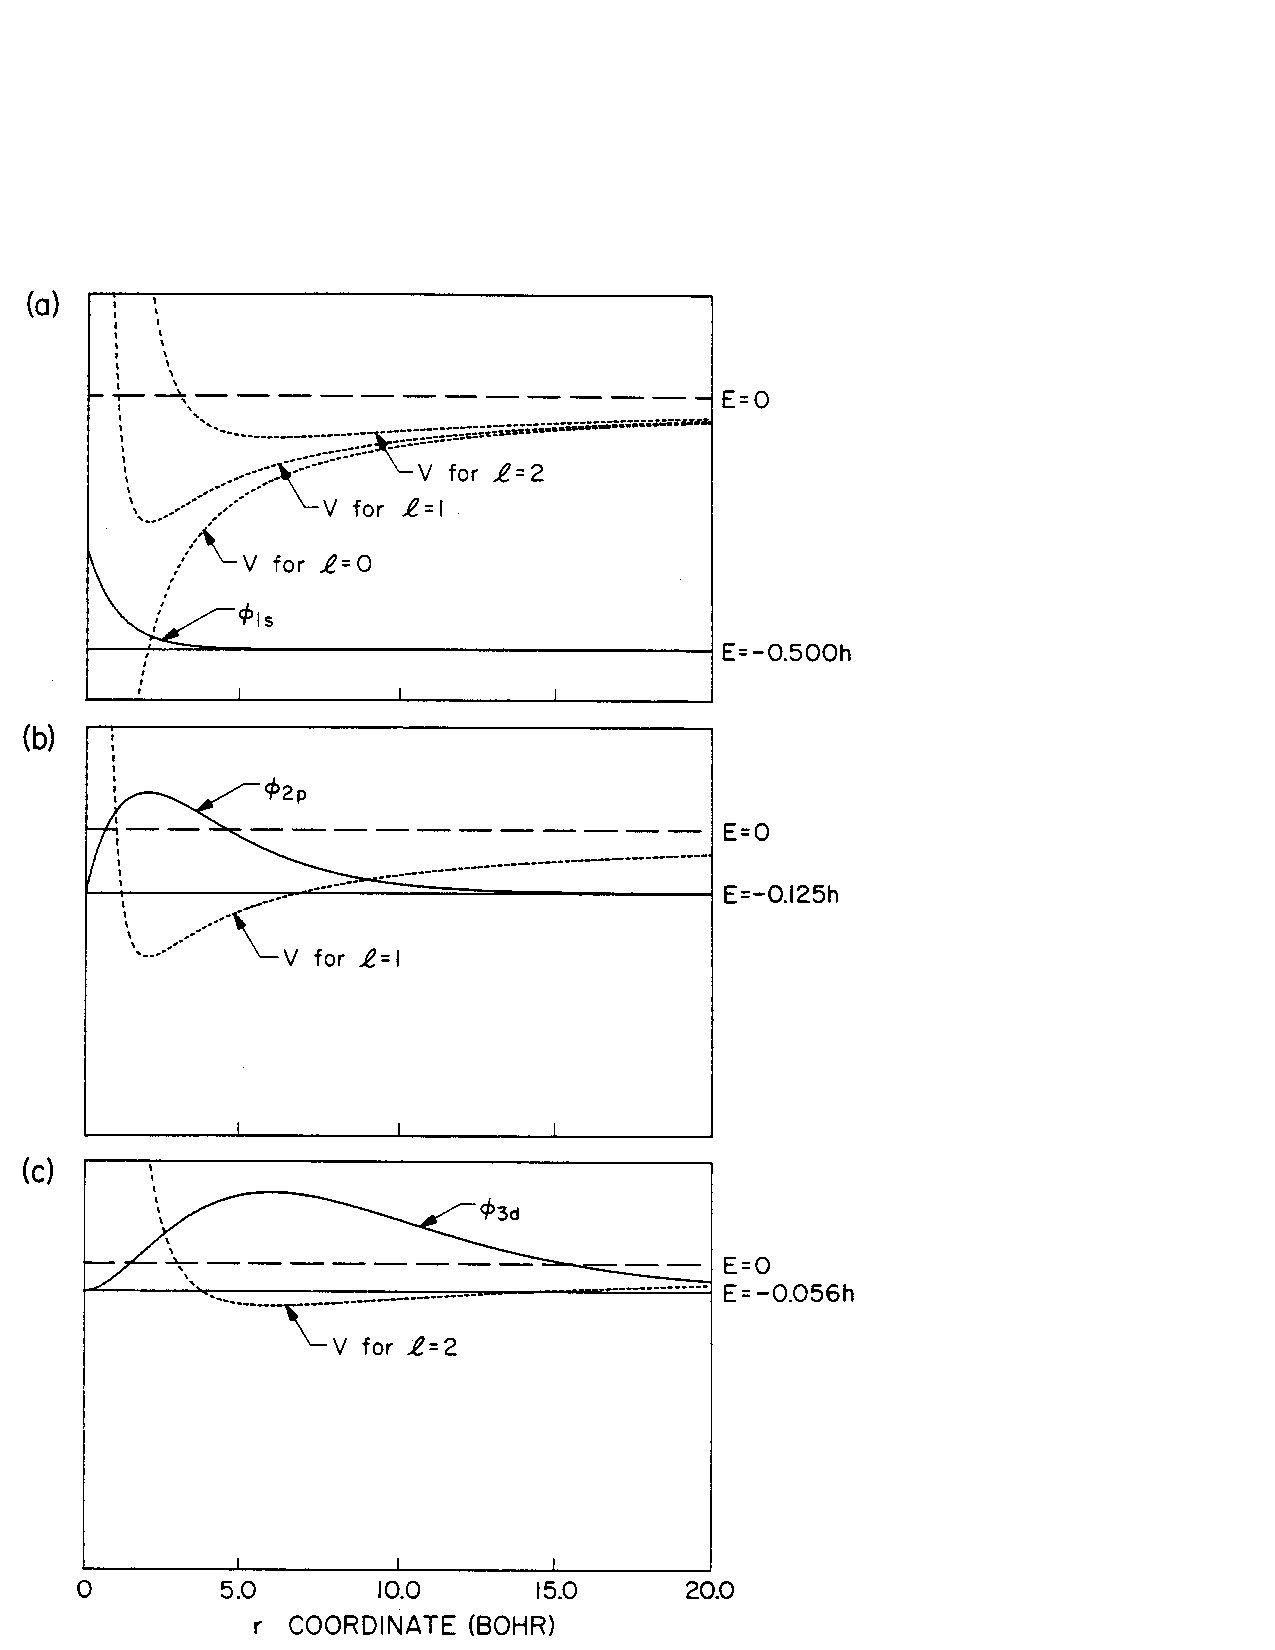
\includegraphics[scale=0.75]{fig5-8}
\caption{Comparison of $1s$, $2p$, and $3s$ orbitals and the
potentials, $V_l$, including centrifugal terms.}
\label{fig5-8}
\end{figure}

\section{The Aufbau Principle of Atoms}

In this section, we develop the Aufbau principle for atoms.  This is based upon
the sequence of states for the H atom, except that inclusion of 
average electron-electron repulsion effects of many-electron atoms, leads to
an ordering of orbitals in this sequence

\begin{tabular}{lll} \\
Row 0 & $1s$ & H to He\cr
Row 1 & $2s$, $3p$ & Li to Ne\cr
Row 2 & $3s$, $3p$ & Na to Ar\cr
Row 3 & $4s$, $3d$, $4p$ & K to Kr\cr
Row 4 & $5s$, $4d$, $5p$ & Rb to Xe\cr
Row 5 & $6s$, $4f$, $5d$, $6p$ & Cs to Rn\cr
Row 6 & $7s$, $5f$, $6d$, $7p$ & Fr to -\cr
\end{tabular}

\noindent
where $1s$ is lowest and large gaps occur between rows. These rows
will be denoted as indicated with Li-Ne as the \emph{first row} (this
is convenient when discussing periodic trends).  The schematic energy
diagram, the \emph{Aufbau diagram}, is given in Figure
\ref{fig5-9}. The ground state of a Z electron atom is thus
constructed by filling these orbitals, 2 electrons per spatial
orbital, starting with the lowest and working up.

\begin{figure}
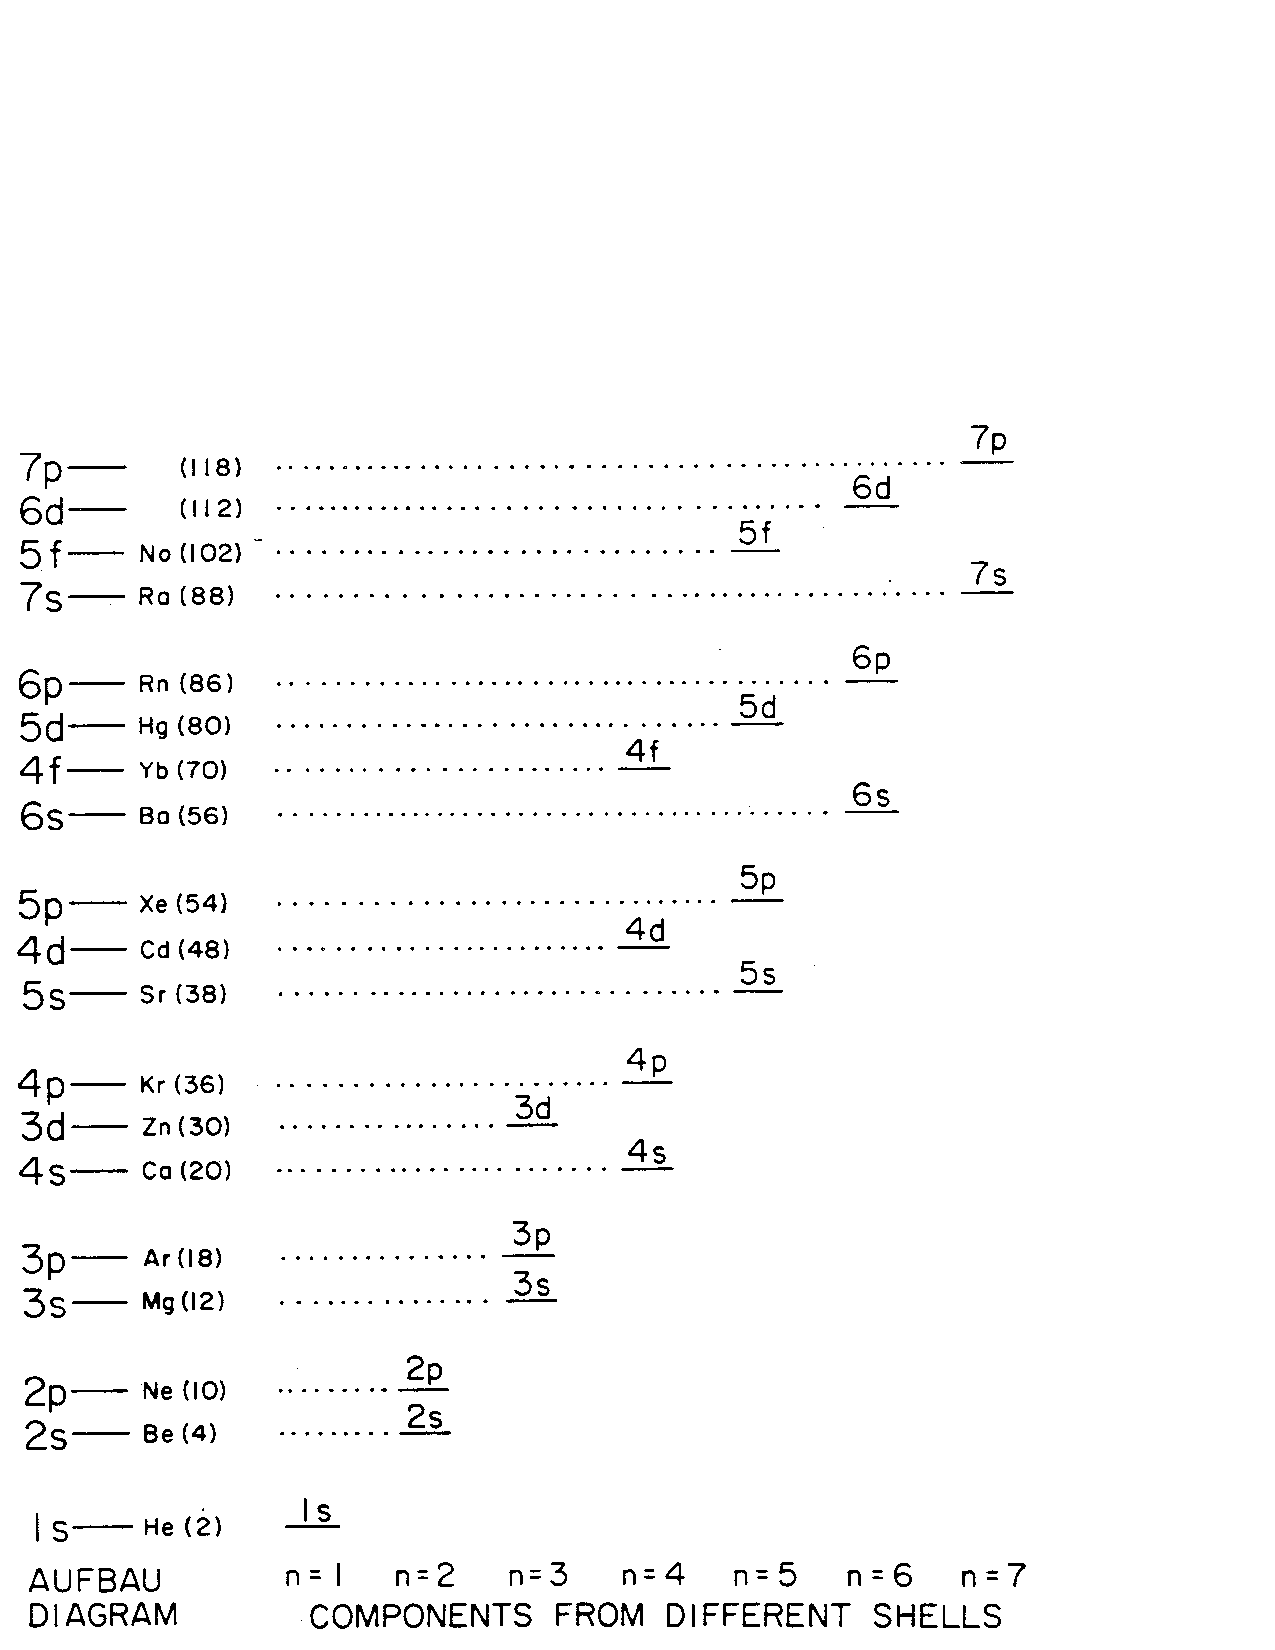
\includegraphics[scale=0.75]{fig5-9}
\caption{The Aufbau diagram.  Also
indicated is the element (Z in parentheses) for which a given
level (and all deeper levels) is filled. The components for different
shells are also listed spearately.}
\label{fig5-9}
\end{figure}

If the highest occupied orbitals are in the r$th$ row, then all
orbitals of the earlier rows are too small to play a special role in
bonding and are referred to as \emph{core orbitals}. The various
occupied orbitals of the r$th$ row are referred to as \emph{valence
orbitals}.  States in different rows, but with the same occupation of
valence orbitals, have similar chemical properties leading to the
\emph{periodic table}, as indicated in Table \ref{chap5-table4} and
\ref{chap5-table5}.

The $d$ and $f$ orbitals complicate the above description. Thus, for
the third row, the $3d$ orbitals are approximately 30 \% the size
of the $4s$ and $4p$ orbitals.  As a result, they play a somewhat
smaller role in the chemistry.  For atoms in which the $d$ and $f$
orbitals are empty, or full, we can generally ignore the $d$ and $f$
orbitals in considering the chemistry.  Thus, Se is analogous to S
despite the $(3d)^{10}$ configuration in Se.  Cases with partially
occupied $d$ or $f$ shells are chemically analogous only to other
cases with similar partial occupations.

The valence orbitals for H through Xe are shown in Figure 10.  The ionization
potentials and electron affinities for various atoms are shown in
Tables \ref{chap5-table4} and \ref{chap5-table5}.

\begin{table}
\caption{}
\label{chap5-table4}
%% Warning! Table 4 and 5 not found!
\end{table}

\begin{table}
\caption{}
\label{chap5-table5}
%% Warning! Table 4 and 5 not found!
\end{table}

Figures \ref{fig5-10a}--\ref{fig5-10g} illustrate the valence orbitals
of H through Xe. In this figure, we plot $r \phi_{nl}$ for the valence
orbitals as obtained from accurate Hartree-Fock calculations. The
bond radius of each atom is indicated by an x on the abscissa,
metallic radius for metal, covalent single-bond radius for nonmetals.
All plots are to the same distance scale.  However, for the Li and Be
columns, an extra piece was added, the vertical dotted line shows
where the cutoff would have been. The same vertical scale is used for
all atoms of the same column. However, different columns may have
different scales, all plots in the same figure have the same vertical
scale.  For the transition elements, Sc-Zn columns, the $4s$ orbital
has been multiplied by three, indicated by *3 in the figure.

\begin{figure}
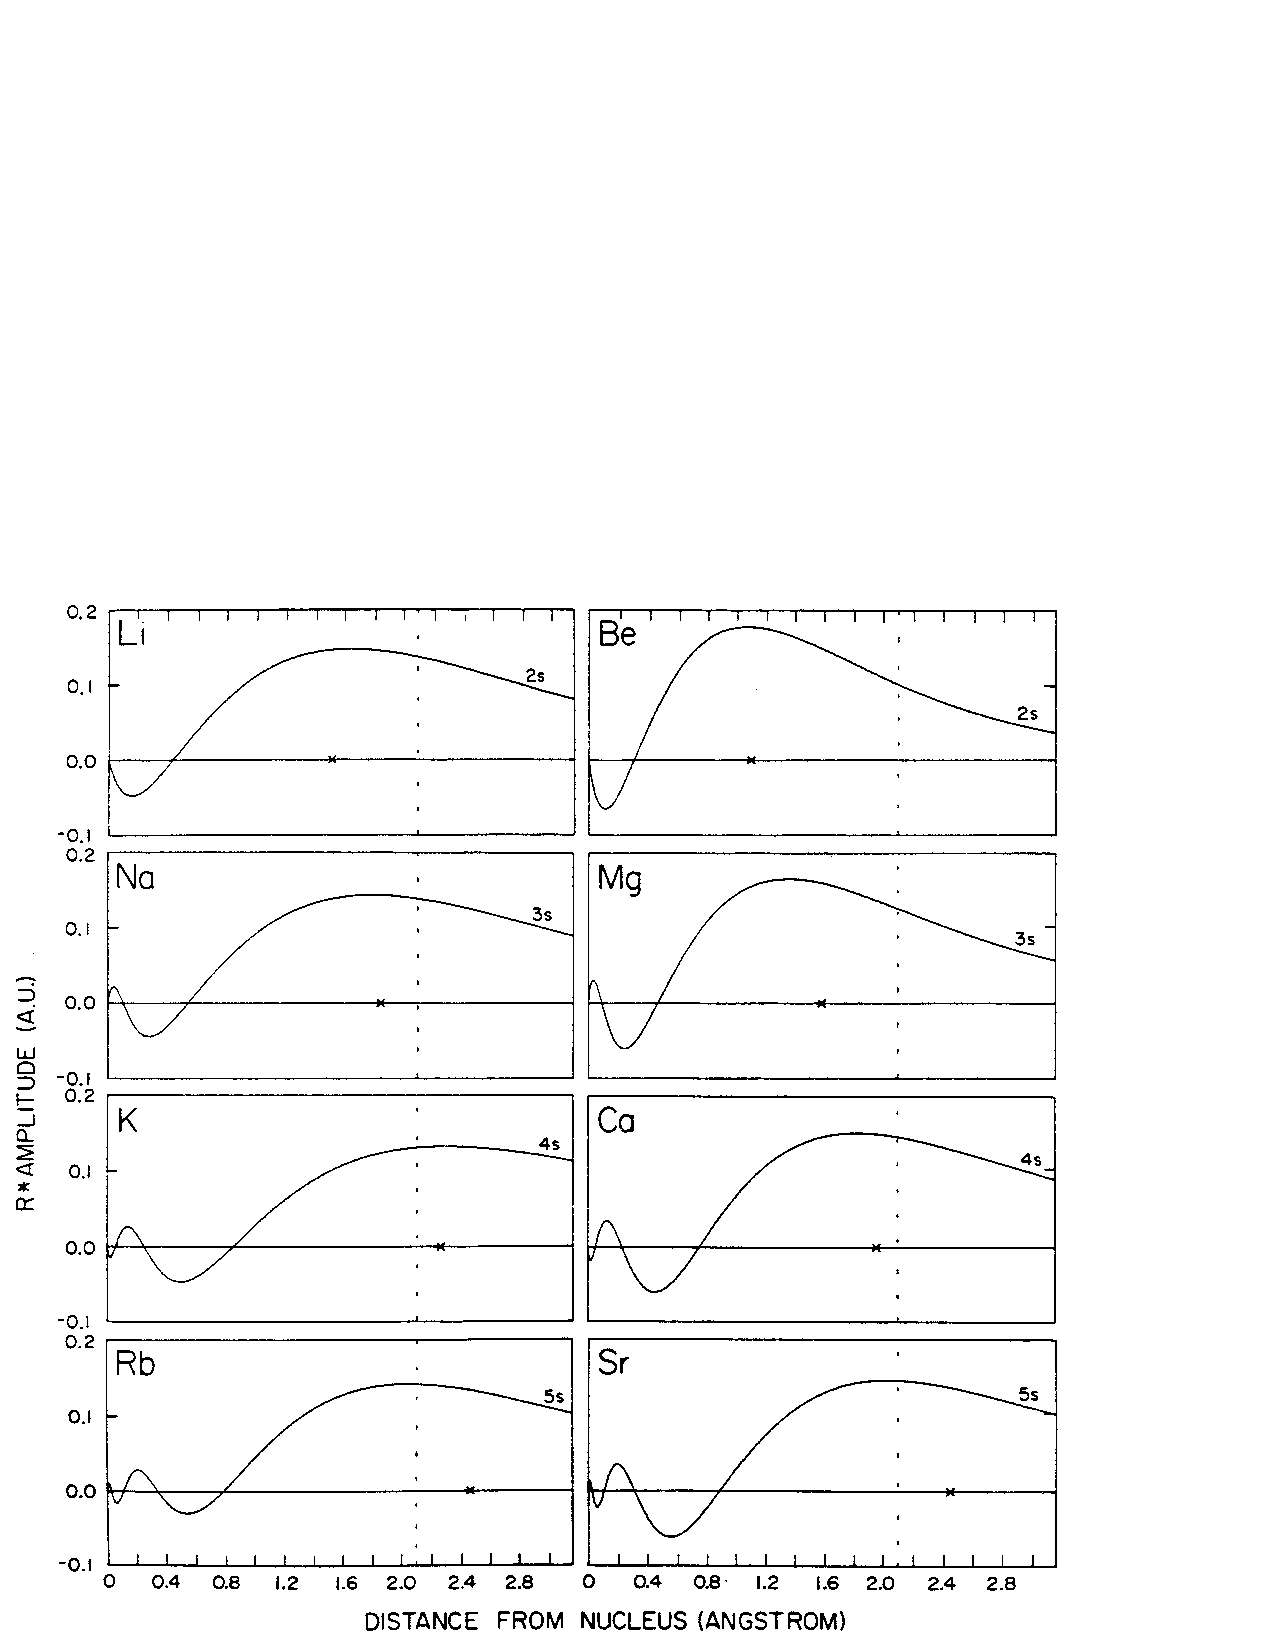
\includegraphics[scale=0.75]{fig5-10a}
\caption{The valence orbitals of alkali and alkali earth metals. We
plot $r \phi_{nl}$ for the valence orbitals as obtained from accurate
Hartree-Fock calculations. The bond radius of each atom is indicated
by an x on the abscissa, metallic radius for metal, covalent
single-bond radius for nonmetals.}
\label{fig5-10a}
\end{figure}

\begin{figure}
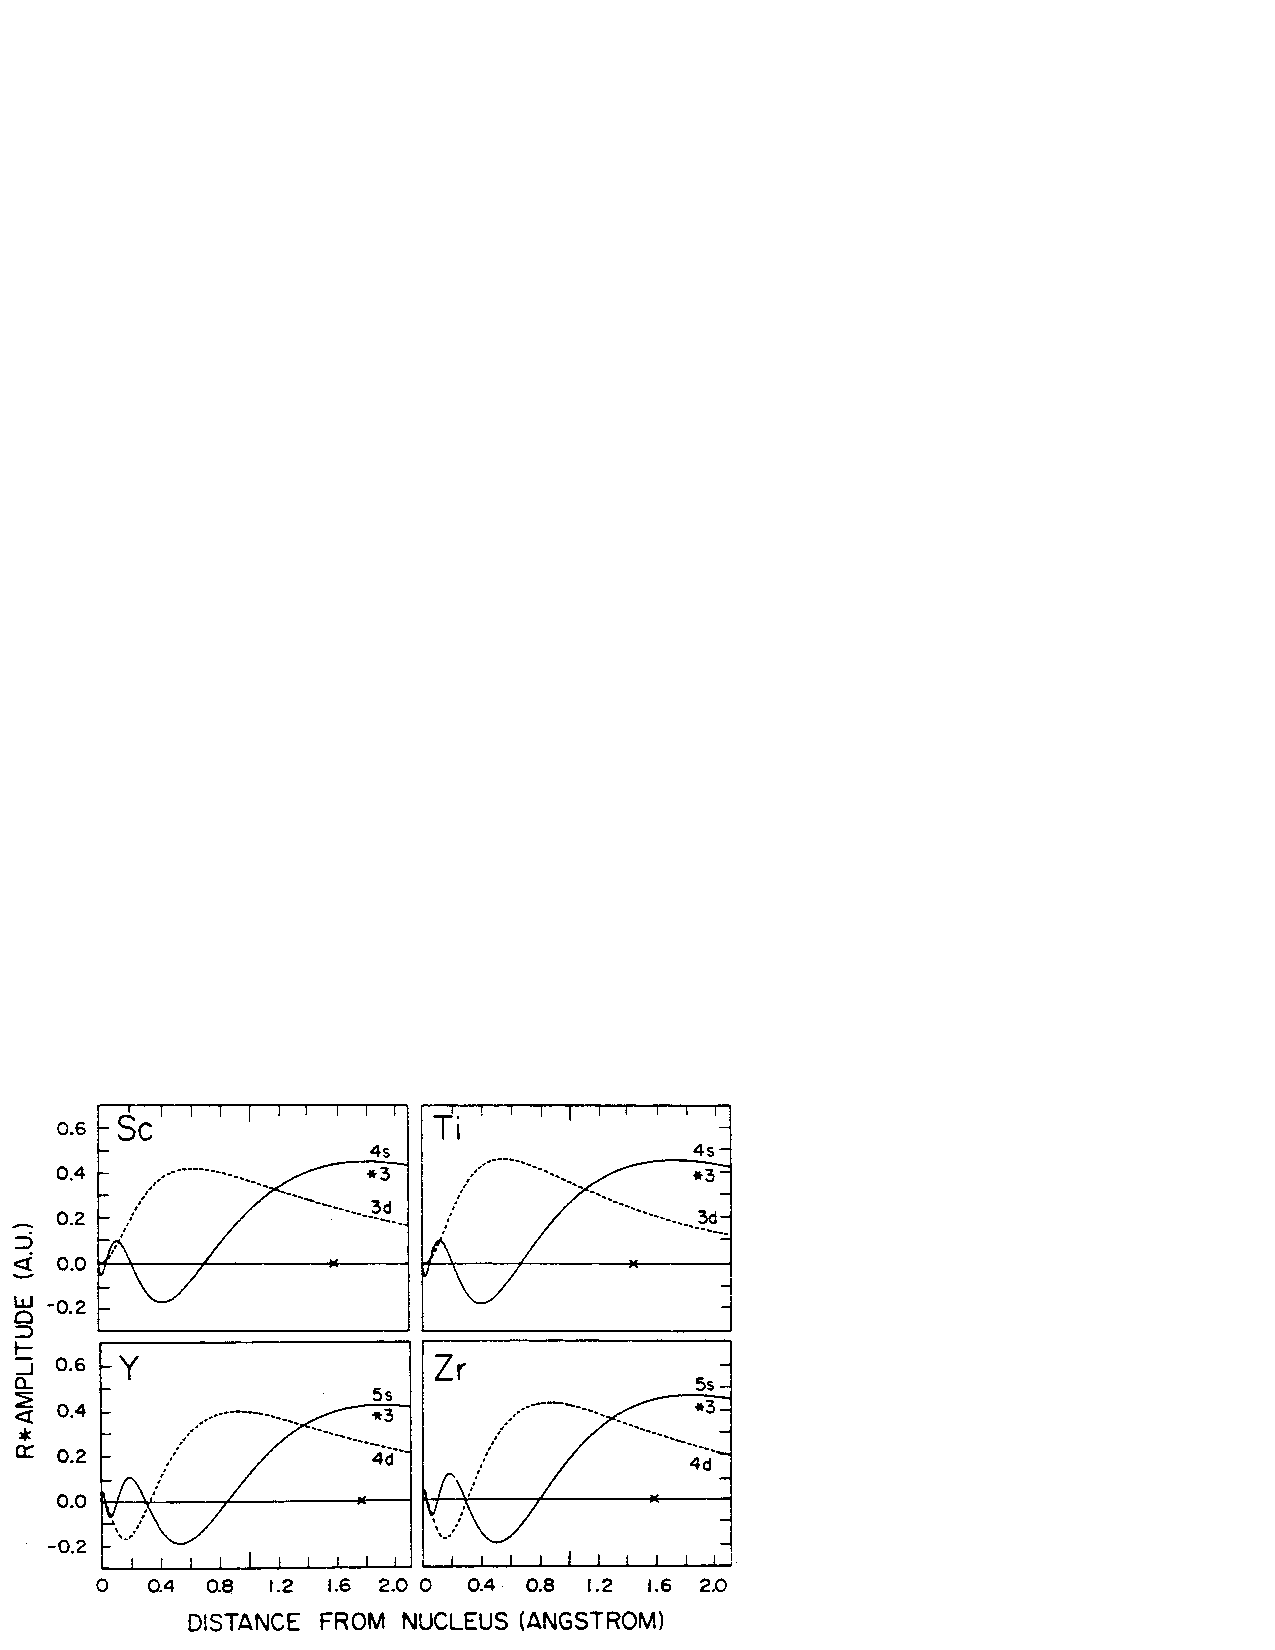
\includegraphics[scale=0.75]{fig5-10b}
\caption{The valence orbitals of early transition metals. We plot $r
  \phi_{nl}$ for the valence orbitals as obtained from accurate
  Hartree-Fock calculations. The bond radius of each atom is indicated
  by an x on the abscissa, metallic radius for metal, covalent
  single-bond radius for nonmetals.}
\label{fig5-10b}
\end{figure}

\begin{figure}
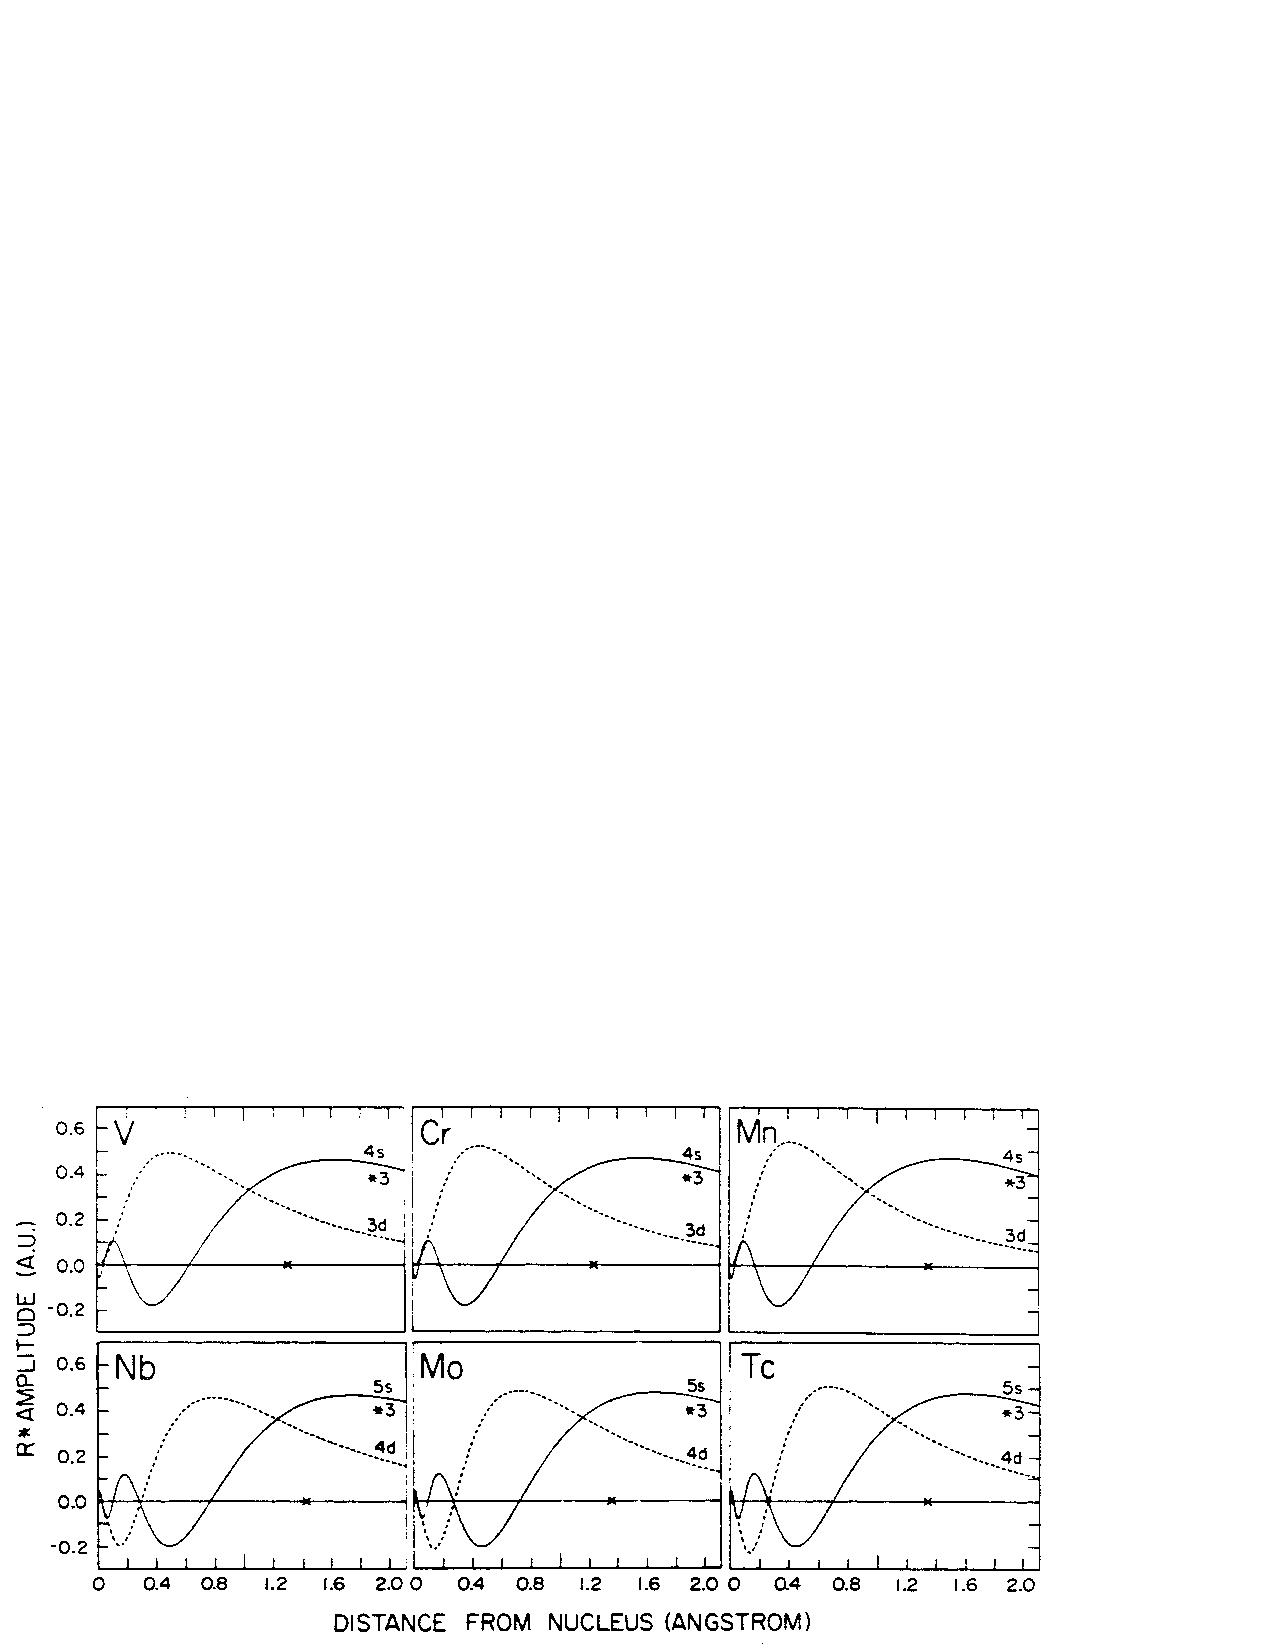
\includegraphics[scale=0.75]{fig5-10c}
\caption{The valence orbitals of middle transition metals. We plot $r
  \phi_{nl}$ for the valence orbitals as obtained from accurate
  Hartree-Fock calculations. The bond radius of each atom is indicated
  by an x on the abscissa, metallic radius for metal, covalent
  single-bond radius for nonmetals.}
\label{fig5-10c}
\end{figure}

\begin{figure}
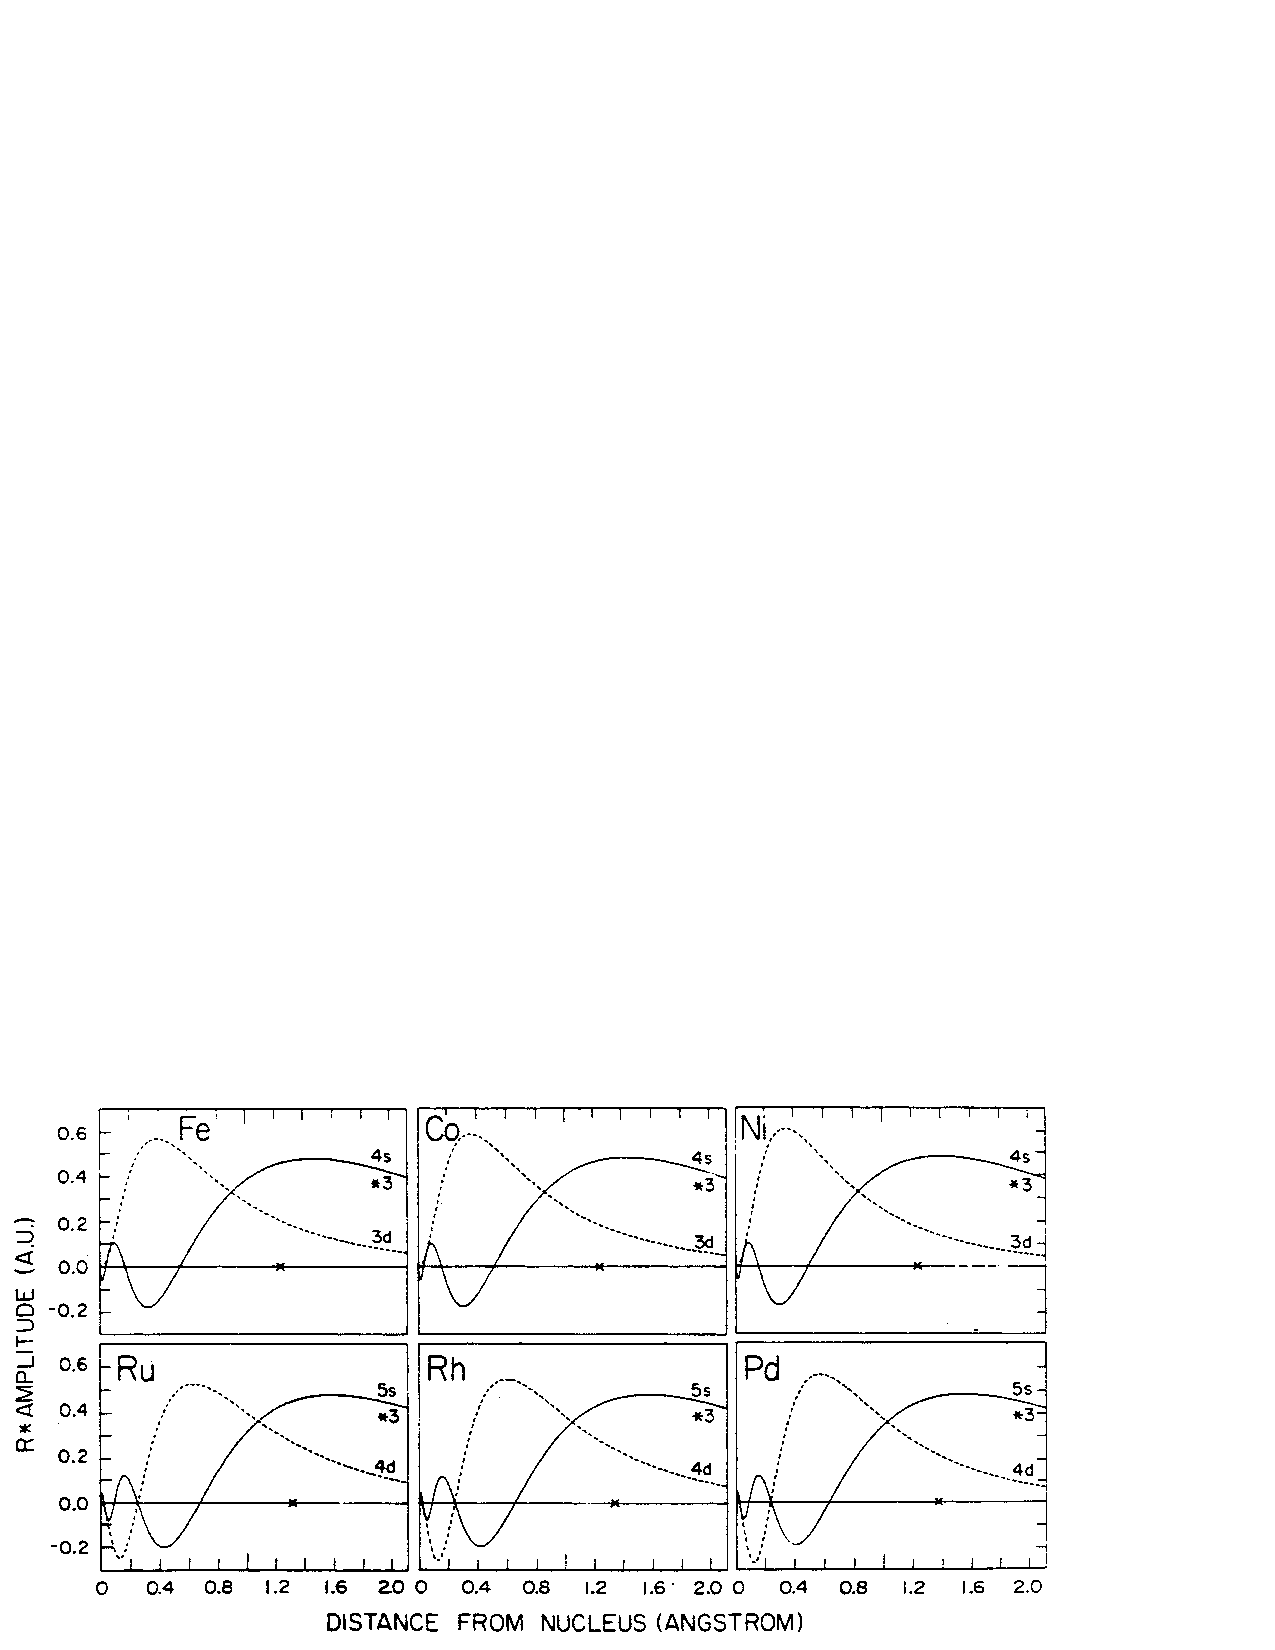
\includegraphics[scale=0.75]{fig5-10d}
\caption{The valence orbitals of late transition metals. We plot $r
  \phi_{nl}$ for the valence orbitals as obtained from accurate
  Hartree-Fock calculations. The bond radius of each atom is indicated
  by an x on the abscissa, metallic radius for metal, covalent
  single-bond radius for nonmetals.}
\label{fig5-10d}
\end{figure}

\begin{figure}
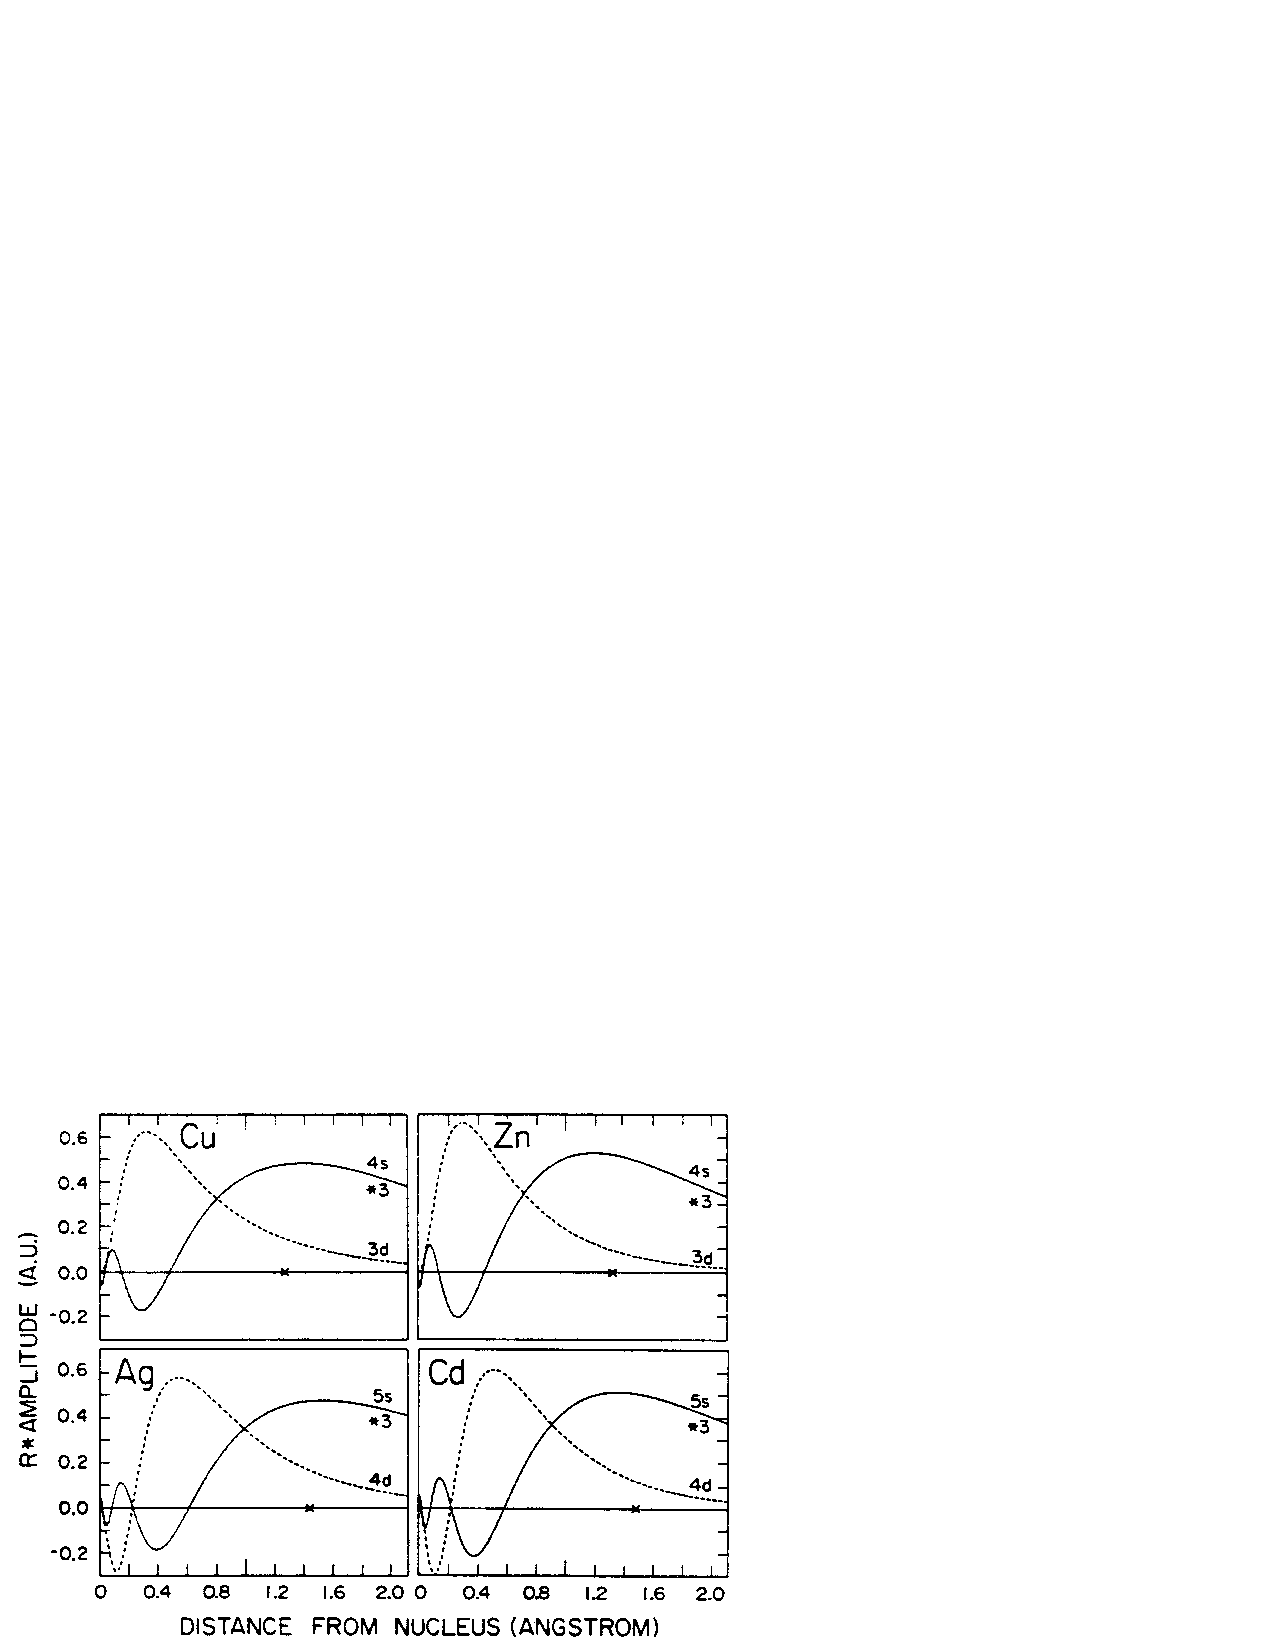
\includegraphics[scale=0.75]{fig5-10e}
\caption{The valence orbitals of Cu, Zn, Ag, and Cd. We plot $r
  \phi_{nl}$ for the valence orbitals as obtained from accurate
  Hartree-Fock calculations. The bond radius of each atom is indicated
  by an x on the abscissa, metallic radius for metal, covalent
  single-bond radius for nonmetals.}
\label{fig5-10e}
\end{figure}

\begin{figure}
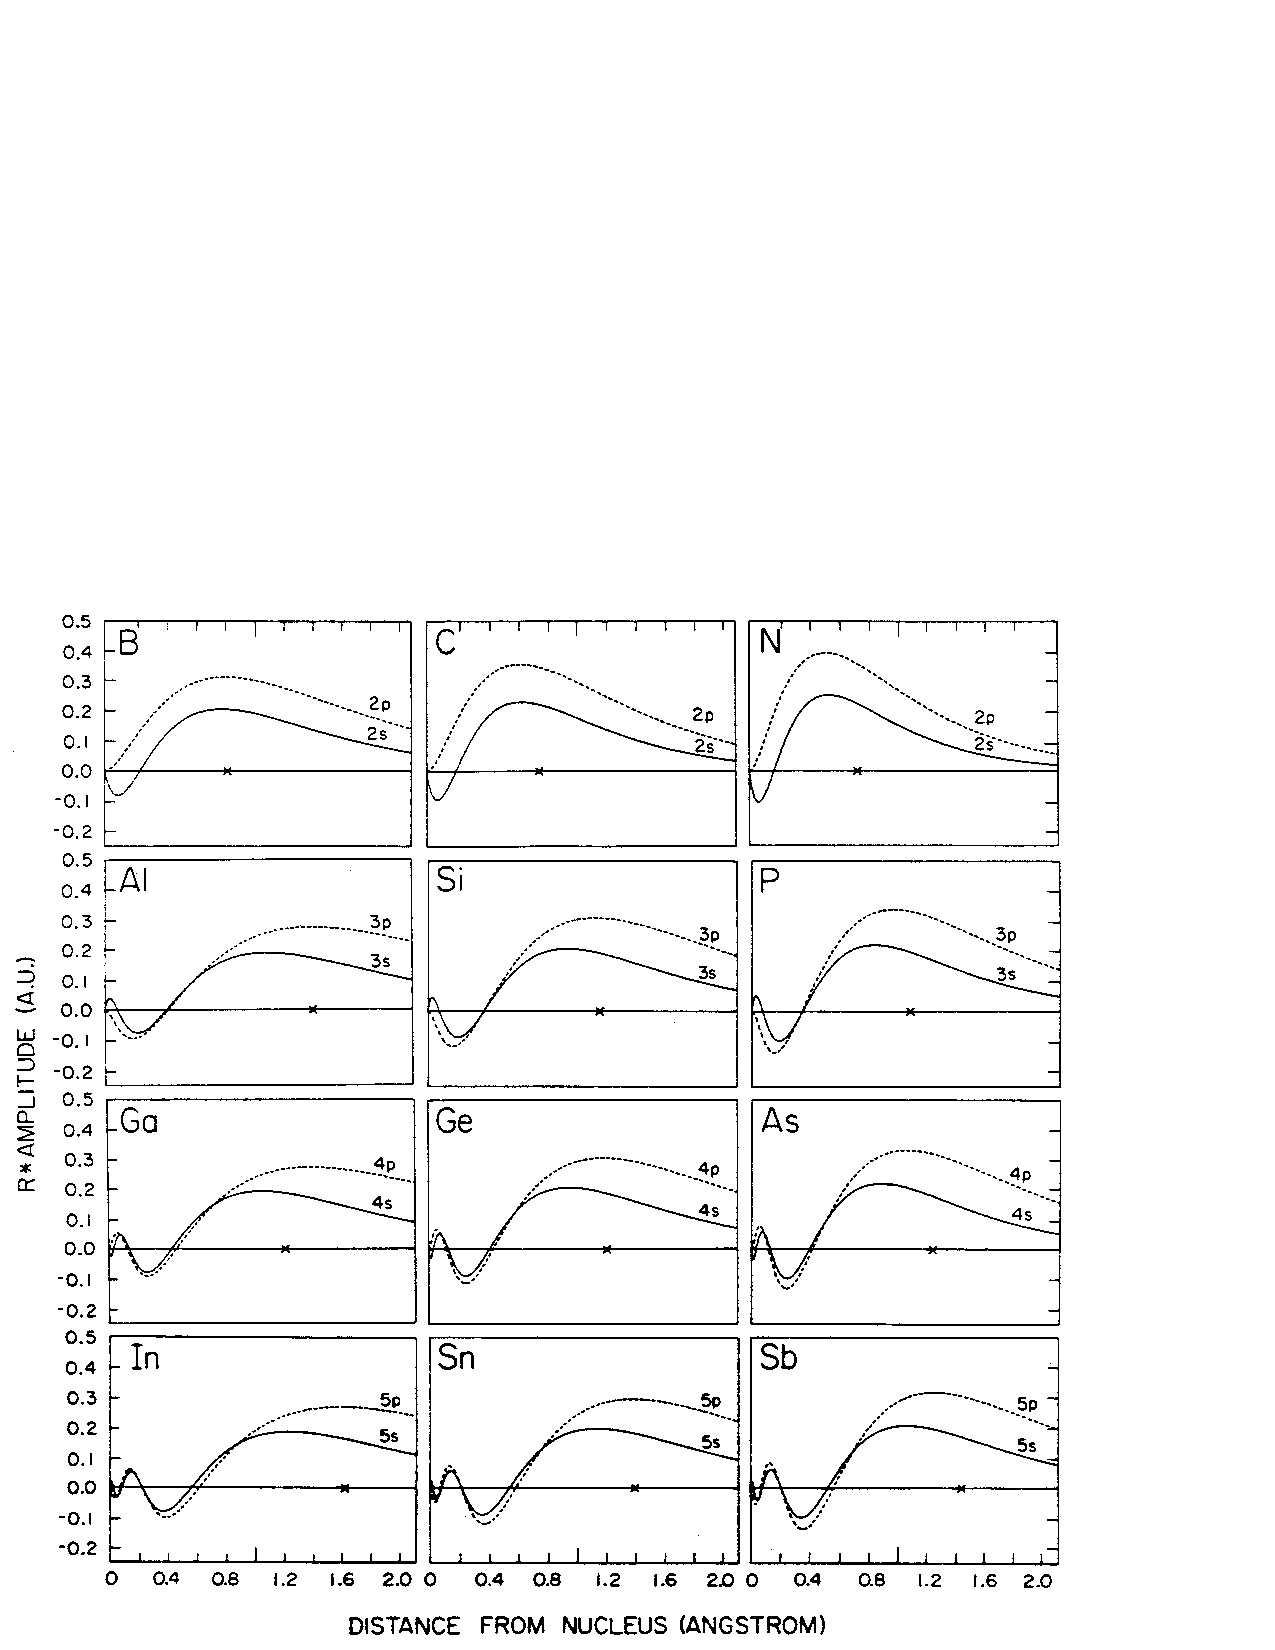
\includegraphics[scale=0.75]{fig5-10f}
\caption{The valence orbitals of main group columns III, IV, and V. We
  plot $r \phi_{nl}$ for the valence orbitals as obtained from
  accurate Hartree-Fock calculations. The bond radius of each atom is
  indicated by an x on the abscissa, metallic radius for metal,
  covalent single-bond radius for nonmetals.}
\label{fig5-10f}
\end{figure}

\begin{figure}
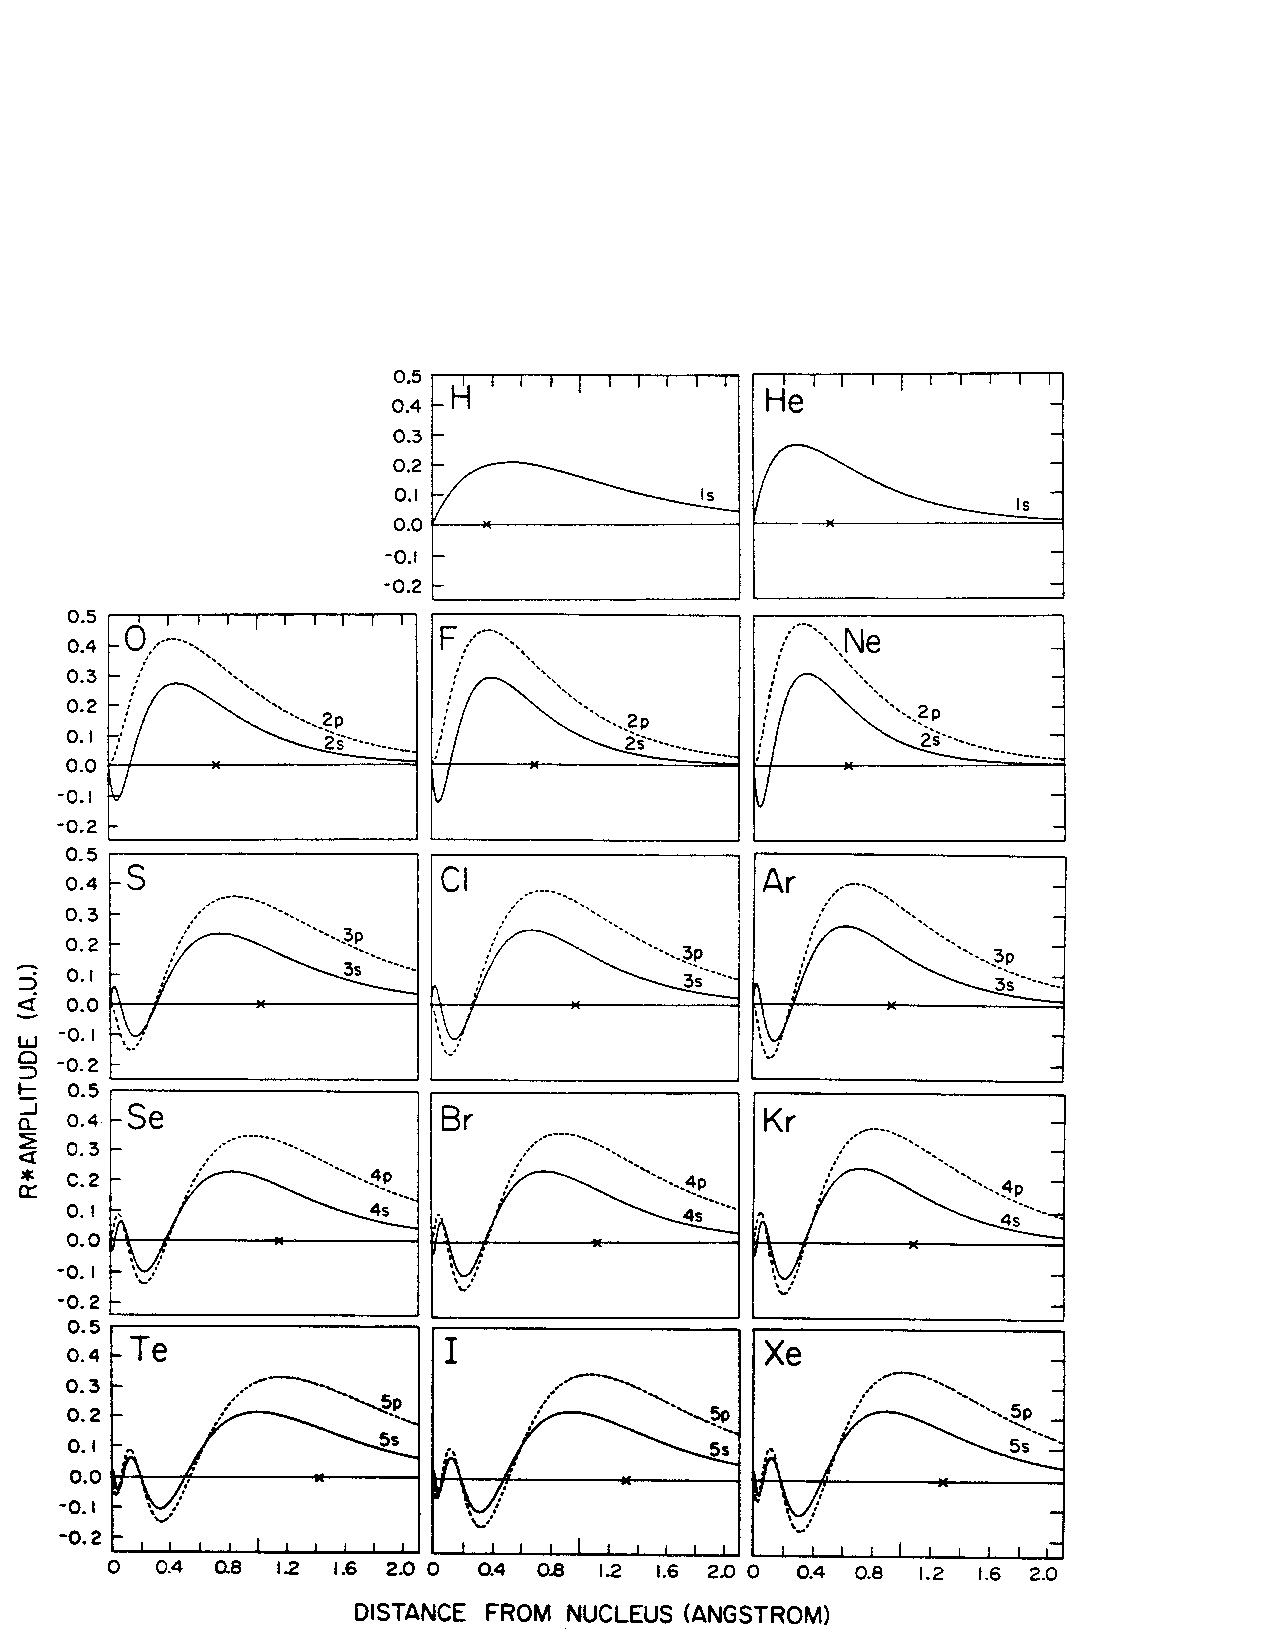
\includegraphics[scale=0.75]{fig5-10g}
\caption{The valence orbitals of main group columns VI, VII, and
  VIII. We plot $r \phi_{nl}$ for the valence orbitals as obtained
  from accurate Hartree-Fock calculations. The bond radius of each
  atom is indicated by an x on the abscissa, metallic radius for
  metal, covalent single-bond radius for nonmetals.}
\label{fig5-10g}
\end{figure}

\subsection{The Ground State Configurations of Atoms}

In Section 5.2 we found that the exact eigenfunctions of the H atom are as 
follows.  For $1s$
\begin{equation}
E = - {1 \over 2h} = - 13.6 {\rm eV}
\end{equation}
For 2s, 2p
\begin{equation}
E = - {1 \over 8} h = - 3.40 {\rm eV}
\end{equation}
For 3s, 3p, and 3d
\begin{equation}
E = - {1 \over 18} h = - 1.51 {\rm eV}
\end{equation}
and for 4s, 4p, 4d, and 4f
\begin{equation}
E = - {1 \over 32} h = - 0.85 {\rm eV}
\end{equation}
with all energies relative to a free electron, plus a proton.  Except for 
scaling of all energies by $Z^2$, the same results are obtained for a 
nucleus of arbitrary $Z$, still one electron, of course.

Now we want to consider a many-electron atom. In the simple
approximation we might completely ignore electron repulsion effects,
placing the electrons in the lowest orbitals, consistent with the
Pauli principle.  In this case, the $Z$ electron atom would be built
up by placing two electrons in the $1s$ orbital, the next eight
electrons in $2s$ and $2p$ orbitals, the next 18 into the $3s$, $3p$,
and $3d$ orbitals, etc.  In this model, there would be a sharp break
after filling each $n$ shell, since the next electron would go in a
much higher orbital. Thus, $Z = 2, 10, 28,$ and 60 would be
particularly stable and ureactive. These $Z$ correspond to He, Ne, Ni,
and Nd, whereas in fact it is He, Ne, Ar, Kr, and Xe that are
particularly stable and unreactive.  Consequently, we must include
electron-electron interaction effects.

Rather than include these electron repulsion effects exactly, we will 
include them in an average way.  Each orbital will be allowed to adjust to 
this average electric field due to the electrons in the other orbitals.

\subsubsection{Effects of Shielding}

Consider, first, the case of a nucleus of charge $Z$ with two
electrons in a $1s$ orbital.  Neglecting electron-electron repulsion,
this optimum $1s$ orbital is $e^{-Zr}$.  Including electron repulsion,
the optimum orbital is $e^{-Z^*r}$ where $Z^* = Z - 5/16$.  Thus, the
average effect of one $1s$ electron upon the other, is equivalent to
cancelling (or \emph{shielding}) 5/16 of a positive charge of the nucleus.

Now consider the Li atom. Two electrons go into the $1s$ orbital, one
with each spin, and the remaining electron goes into an $n = 2$
orbital, $2s$ or $2p$ orbital. If the density for the $n = 2$ orbital
were entirely outside the density of the $1s$ orbital, then the
optimum $Z^*$ for the $1s$ orbital would be unchanged by the $n = 2$
orbital, while the $1s$ electrons would completely shield two protons
from the $n = 2$ orbital.  Thus, we would obtain
\begin{equation}
Z^*_{1s} = 3 - {5 \over 16} = 2.69
\end{equation}
\begin{equation}
Z^*_{2s} = Z^*_{2p} = 3 - 2 = 1.
\end{equation}
In fact, this is a good approximation for the $2p$ orbital since this
orbital goes to zero at the nucleus. However, the $2s$ orbital is
nonzero at the nucleus and has a significant density within the $1s$
region.  As a result, the $1s$ electrons only partially shield the
nucleus.  The result is, for Li
\begin{equation}
Z^*_{1s} = 3 - {5 \over 16} = 2.69
\end{equation}
\begin{equation}
Z^*_{2s} = 3 - 1.72 = 1.28
\end{equation}
\begin{equation}
Z^*_{2p} = 3 - 2 = 1.00 .
\end{equation}
Since the nucleus is less completely shielded from the $2s$ orbital than 
from $2p$, the $2s$ orbital is more strongly bound than $2p$, and hence, the 
ground state of Li is $(1s)^2 (2s)^1$, while $(1s)^2 (2p)^1$ is the 
first excited states, 2 eV excitation energy.

Similar differential shielding effects lead to a splitting of the various 
$nl$ states of H atom, having the same $n$ with the result that for 
many-electron atoms, the energies satisfy
\begin{equation}
2s < 2p ,
\end{equation}
\begin{equation}
3s < 3p < 3d ,
\end{equation}
\begin{equation}
4s < 4p < 4d < 4f ,
\end{equation}
etc.  In all cases, higher $l$ leads to less penetration of the core,
resulting in greater shielding by the core orbitals, leading thereby
to higher energy.  These $l$-splitting effects depend somewhat upon
the precise occupation of the various orbitals, but the ground states
of most atoms can be qualitatively explained by the simple
\emph{Aufbau diagram} in Figure \ref{fig5-9}.  Magnitudes of the
separations in the Aufbau diagram are not to scale.

As illustrated, the $l$-splitting is sometimes larger than the $n$ 
splitting, resulting in the general sequences
\begin{eqnarray}
&& 1s,\cr
&& 2s,2p,\cr
&& 3s,3p\cr
&& 4s,3d,4p\cr
&& 5s,4d,5p,\cr
&& 6s,4f,5d,6p\cr
&& 7s,5f,6d,7p
\label{chap5-eqno15}
\end{eqnarray}
where we have used separate rows to indicate a big break after 
filling the $np$ orbital of each row.

\subsubsection{The Aufbau Principle}

Using the ordering of levels in (\ref{chap5-eqno15}), or Figure
\ref{fig5-9}, leads to the Aufbau principle. For an atom of atomic
number $Z$, we fill in the lowest orbitals in Figure \ref{fig5-9},
allowing 2 electrons per orbital, until all electrons are used
up. Counting spatial degeneracies, this allows two electrons for $s$
shell, six electrons for $p$ shell, ten electrons for $d$ shells, and
fourteen electrons for $f$ shells.  For example, this leads to
\begin{eqnarray}
Z &=& 2, {\rm He} : (1s)^2\cr
Z &=& 6, {\rm C} : ( {\rm He} )   (2s)^2 (2p)^2\cr
Z &=& 10, {\rm Ne} : ( {\rm He} ) (2s)^2 (2p)^6\cr
Z &=& 18, {\rm Ar} : ( {\rm Ne} ) (3s)^2 (3p)^6\cr
Z &=& 26, {\rm Fe} : ( {\rm Ar} ) (4s)^2 (3d)^6\cr
Z &=& 36, {\rm Kr} : ( {\rm Ar} ) (4s)^2 (3d)^{10} (4p)^6\cr
Z &=& 54, {\rm Xe} : ( {\rm Kr} ) (5s)^2 (4d)^{10} (5p)^6\cr
Z &=& 86, {\rm Rn} : ( {\rm Xe} ) (6s)^2 (4f)^{14} (5d)^{10} (6p)^6,
\end{eqnarray}
where the configuration of the core electrons is indicated by the 
corresponding atomic symbol, for example (Ar) indicates the configuration 
of, ground state, Ar.  Large gaps occur after the $1s$, $2p$, $3p$, 
$4p$, $5p$, and $6p$, shells are filled, resulting in particularly unreactive 
and stable atoms, the noble gases of He, Ne, Ar, Kr, Xe, and Rn.

\begin{table}
\caption{The ground configurations for atoms H-Ar.  Also 
included is the term for the ground state and the ionization
potential.}
\label{chap5-table6}
\begin{tabular}{rrlccc} \\ \hline
   & Z   & Configuration   & Symmetry & Lowest Orb$^a$ & IP (eV)$^a$\cr

H  & 1   & $(1s)$    & ${^2S}_{g{1 \over 2}}$ & $1s$ & 13.595\cr
He & 2   & $(1s)^2$  & ${^1S}_{g0}$ & 1s & 24.481\cr
Li & 3   & $(1s)^2(2s)$    & ${^2S}_{g{1 \over 2}}$ & $2s$ & 5.390\cr
Be & 4   & $(1s)^2(2s)^2$    & ${^1S}_{g0}$ & 2s & 9.320\cr
B  & 5   & $(1s)^2(2s)(2p)$    & ${^2P}_{u{1 \over 2}}$ & $2p$ & 8.296\cr
C  & 6   & $(1s)^2(2s)(2p)^2$    & ${^3P}_{g0}$ & 2p & 11.256\cr
N  & 7   & $(1s)^2(2s)(2p)^3$    & ${^4S}_{u{3 \over 2}}$ & $2p$ & 14.53\cr
O  & 8   & $(1s)^2(2s)(2p)^4$    & ${^3P}_{g2}$ & 2p & 13.614\cr
F  & 9   & $(1s)^2(2s)(2p)^5$    & ${^2P}_{u{3 \over 2}}$ & $2p$ & 17.418\cr
Ne & 10  & $(1s)^2(2s)(2p)^6$    & ${^1S}_g$ & $2p$ & 21.559\cr
Na & 11  & (Ne)$(3s)$    & ${^2S}_{g{1 \over 2}}$ & $3s$ & 5.138\cr
Mg & 12  & (Ne)$(3s)^2$    & ${^1S}_{g0}$ & $3s$ & 7.644\cr
Al & 13  & (Ne)$(3s)^2(3p)$    & ${^2P}_{u{1 \over 2}}$ & $3p$ & 5.984\cr
Si & 14  & (Ne)$(3s)^2(3p)^2$    & ${^3P}_{g0}$ & $3p$ & 8.149\cr
P  & 15  & (Ne)$(3s)^2(3p)^3$    & ${^4S}_{u{3 \over 2}}$ & $3p$ & 10.484\cr
S  & 16  & (Ne)$(3s)^2(3p)^4$    & ${^3P}_{g2}$ & $3p$ & 10.357\cr
Cl & 17  & (Ne)$(3s)^2(3p)^5$    & ${^2P}_{u{3 \over 2}}$ & $3p$ & 13.01\cr
Ar & 18  & (Ne)$(3s)^2(3p)^6$    & ${^1S}_{g0}$ & $3p$ & 15.755\cr
\hline
\end{tabular}
\end{table}

\begin{table}
\caption{The ground configurations for atoms K-Kr.  Also 
included is the term for the ground state and the ionization
potential.}
\label{chap5-table6a}
\begin{tabular}{rrlccc} \\ \hline
   & Z   & Configuration   & Symmetry & Lowest Orb$^a$ & IP (eV)$^a$\cr

K  & 19  & (Ar)$(4s)$    & ${^2S}_{g{1 \over 2}}$ & $4s$ & 4.339\cr
Cs & 20  & (Ar)$(4s)^2$    & ${^1S}_{g0}$ & $4s$ & 6.111\cr
Sc & 21  & (Ar)$(4s)^2(3d)$    & ${^2D}_{g{3 \over 2}}$ & $4s$ & 6.54\cr
Ti & 22  & (Ar)$(4s)^2(3d)^2$    & ${^3F}_{g2}$ & $4s$ & 6.82\cr
V  & 23  & (Ar)$(4s)^2(3d)^3$    & ${^4F}_{g{3 \over 2}}$ & $b$ & 6.74\cr
Cr & 24  & (Ar)$(4s)^2(3d)^4$    & ${^7S}_{g3}$ & $4s$ & 6.764\cr
Mn & 25  & (Ar)$(4s)^2(3d)^5$    & ${^6S}_{g{5 \over 2}}$ & $4s$ & 7.432\cr
Fe & 26  & (Ar)$(4s)^2(3d)^6$    & ${^5D}_{g4}$ & $4s$ & 7.87\cr
Co & 27  & (Ar)$(4s)^2(3d)^7$    & ${^4F}_{g{9 \over 2}}$ & $c$ & 7.86\cr
Ni & 28  & (Ar)$(4s)^2(3d)^8$    & ${^3F}_{g4}$ & $d$ & 7.633\cr
Cu & 29  & (Ar)$(4s)(3d)^{10}$    & ${^2S}_{g{1 \over 2}}$ & $4s$ & 7.724\cr
Zn & 30  & (Ar)$(4s)^2(3d)^{10}$    & ${^1S}_{g0}$ & $4s$ & 9.391\cr
Ga & 31  & (Ar)$(4s)^2(3d)^{10}(4p)$    & ${^2P}_{u{1 \over 2}}$ & $4p$ & 6.00\cr
Ge & 32  & (Ar)$(4s)^2(3d)^{10}(4p)^2$    & ${^3P}_{g0}$ & $4p$ & 7.88\cr
As & 33  & (Ar)$(4s)^2(3d)^{10}(4p)^3$    & ${^4S}_{u{3 \over 2}}$ & $4p$ & 9.81\cr
Se & 34  & (Ar)$(4s)^2(3d)^{10}(4p)^4$    & ${^3P}_{g0}$ & $4p$ & 9.75\cr
Br & 35  & (Ar)$(4s)^2(3d)^{10}(4p)^5$    & ${^2P}_{u{3 \over 2}}$ & $4p$ & 11.84\cr
Kr & 36  & (Ar)$(4s)^2(3d)^{10}(4p)^6$    & ${^1S}_{g0}$ & $4p$ & 13.996\cr
\hline
\end{tabular}
\end{table}

\begin{table}
\caption{The ground configurations for atoms Rb-Xe.  Also 
included is the term for the ground state and the ionization
potential.}
\label{chap5-table6b}
\begin{tabular}{rrlccc} \\ \hline
   & Z   & Configuration   & Symmetry & Lowest Orb$^a$ & IP (eV)$^a$\cr

Rb & 37  & (Kr)$(5s)$    & ${^2S}_{g{1 \over 2}}$ & $5s$ & 4.176\cr
Sr & 38  & (Kr)$(5s)^2$    & ${^1S}_{g0}$ & $5s$ & 5.692\cr
Y  & 39  & (Kr)$(5s)^2(4d)$    & ${^2D}_{g{3 \over 2}}$ & $4d$ & 6.38\cr
Zr & 40  & (Kr)$(5s)^2(4d)^2$    & ${^3F}_{g2}$ & $5s$ & 6.84\cr
Nb & 41  & (Kr)$(5s)^1(4d)^4$    & ${^6D}_{g{1 \over 2}}$ & $5s$ & 6.88\cr
Mo & 42  & (Kr)$(5s)^1(4d)^5$    & ${^7S}_{g3}$ & $5s$ & 7.10\cr
Tc & 43  & (Kr)$(5s)^2(4d)^5$    & ${^6S}_{g{5 \over 2}}$ & $5s$ & 7.28\cr
Ru & 44  & (Kr)$(5s)^1(4d)^7$    & ${^5F}_{g5}$ & $5s$ & 7.364\cr
Rh & 45  & (Kr)$(5s)^1(4d)^8$    & ${^4F}_{g{9 \over 2}}$ & $5s$ & 7.46\cr
Pd & 46  & (Kr)$(5s)^0(4d)^{10}$    & ${^1S}_{g9}$ & $4d$ & 8.33\cr
Ag & 47  & (Kr)$(5s)^1(4d)^{10}$    & ${^2S}_{g{1 \over 2}}$ & $5s$ & 7.574\cr
Cd & 48  & (Kr)$(5s)^2(4d)^{10}$    & ${^1S}_{g0}$ & $5s$ & 8.991\cr
In & 49  & (Kr)$(5s)^2(4d)^{10}(5p)$    & ${^2P}_{u{1 \over 2}}$ & $5p$ & 5.785\cr
Sn & 50  & (Kr)$(5s)^2(4d)^{10}(5p)^2$    & ${^3P}_{g0}$ & $5p$ & 7.342\cr
Sb & 51  & (Kr)$(5s)^2(4d)^{10}(5p)^3$    & ${^4S}_{u{3 \over 2}}$ & $5p$ & 8.639\cr
Te & 52  & (Kr)$(5s)^2(4d)^{10}(5p)^4$    & ${^3P}_{g2}$ & $5p$ & 9.01\cr
I  & 53  & (Kr)$(5s)^2(4d)^{10}(5p)^5$    & ${^2P}_{u{3 \over 2}}$ & $5p$ & 10.454\cr
Xe & 54  & (Kr)$(5s)^2(4d)^{10}(5p)^6$    & ${^1S}_{g0}$ & $5p$ & 12.127\cr
\hline
\end{tabular}
\end{table}

\begin{table}
\caption{The ground configurations for atoms Cs-Rn.  Also 
included is the term for the ground state and the ionization
potential.}
\label{chap5-table6c}
\begin{tabular}{rrlccc} \\ \hline
   & Z   & Configuration   & Symmetry & Lowest Orb$^a$ & IP (eV)$^a$\cr

Cs & 55  & (Xe)$(6s)$    & ${^2S}_{g{1 \over 2}}$& $6s$ &3.893\cr
Ba & 56  & (Xe)$(6s)^2$    & ${^1S}_{g0}$& $6p$ &5.21\cr
La & 57  & (Xe)$(6s)^2(5d)$    & ${^2D}_{g{3 \over 2}}$&$e$&5.61\cr
Ce & 58  & (Xe)$(6s)^2(4f)^2$    & $6p$ &5.6\cr
Pr & 59  & (Xe)$(6s)^2(4f)^3$    & $6p$ &5.46\cr
Nd & 60  & (Xe)$(6s)^2(4f)^4$    & ${^5I}_{g4}$ & $6p$ & 5.51\cr
Pm & 61  & (Xe)$(6s)^2(4f)^5$    & $6p$ & -\cr
Sm & 62  & (Xe)$(6s)^2(4f)^6$    & ${^7F}_{g0}$ & $6p$ & 5.6\cr
Eu & 63  & (Xe)$(6s)^2(4f)^7$    & ${^8S}_{u{7 \over 2}}$ & $6p$ & 5.67\cr
Gd & 64  & (Xe)$(6s)^2(4f)^7(5d)$    & ${^9D}_{u2}$ & $6p$ & 6.16\cr
Tb & 65  & (Xe)$(6s)^2(4f)^9$    & $6p$ & 5.98\cr
Dy & 66  & (Xe)$(6s)^2(4f)^{10}$    & $6p$&6.8\cr
Ho & 67  & (Xe)$(6s)^2(4f)^{11}$    & $6p$ & -\cr
Er & 68  & (Xe)$(6s)^2(4f)^{12}$    & $6p$ & 6.08\cr
Tm & 69  & (Xe)$(6s)^2(4f)^{13}$    & ${^2F}_{u{7 \over 2}}$ & $6p$ & 5.81\cr
Yb & 70  & (Xe)$(6s)^2(4f)^{14}$    & ${^1S}_{g0}$ & $6p$ & 6.2\cr
Lu & 71  & (Xe)$(6s)^2(4f)^{14}(5d)$    & ${^2D}_{g{5 \over 2}}$ & $6p$ & -\cr
Hf & 72  & (Xe)$(6s)^2(4f)^{14}(5d)^2$    & ${^3F}_{g2}$ & $5d$ & 7\cr
Ta & 73  & (Xe)$(6s)^2(4f)^{14}(5d)^3$    & ${^4F}_{g{3 \over 2}}$ & $6s$ & 7.88\cr
W  & 74  & (Xe)$(6s)^2(4f)^{14}(5d)^4$    & ${^5D}_{g0}$ & $6s$ & 7.96\cr
Re & 75  & (Xe)$(6s)^2(4f)^{14}(5d)^5$    & ${^6S}_{g{5 \over 2}}$ & $6s$ & 7.87\cr
Os & 76  & (Xe)$(6s)^2(4f)^{14}(5d)^6$    & ${^5D}_{g4}$ & $6s$ & 8.5\cr
Ir & 77  & (Xe)$(6s)^2(4f)^{14}(5d)^7$    & ${^4F}_{g{3 \over 2}}$ & $6s$ & 9\cr
Pt & 78  & (Xe)$(6s)(4f)^{14}(5d)^9$    & ${^3D}_{g3}$ & $6s$ & 9.0\cr
Au & 79  & (Xe)$(6s)(4f)^{14}(5d)^{10}$    & ${^2S}_{g{1 \over 2}}$&$6s$&9.22\cr
Hg & 80  & (Xe)$(6s)^2(4f)^{14}(5d)^{10}$    & ${^1S}_{g0}$&$6s$&10.43\cr
Tl & 81  & (Xe)$(6s)^2(4f)^{14}(5d)^{10}(6p)$    & ${^2P}_{u{1 \over 2}}$&$6p$&6.106\cr
Pb & 82  & (Xe)$(6s)^2(4f)^{14}(5d)^{10}(6p)^2$    & ${^3P}_{g0}$ & $6p$ & 7.415\cr
Bi & 83  & (Xe)$(6s)^2(4f)^{14}(5d)^{10}(6p)^3$    & ${^4S}_{u{3 \over 2}}$&$6p$&7.287\cr
Po & 84  & (Xe)$(6s)^2(4f)^{14}(5d)^{10}(6p)^4$    & $6p$&9.43\cr
At & 85  & (Xe)$(6s)^2(4f)^{14}(5d)^{10}(6p)^5$    & $6p$&9.5\cr
Rn & 86  & (Xe)$(6s)^2(4f)^{14}(5d)^{10}(6p)^6$    & ${^1S}_{g0}$&$6p$&10.746\cr
\hline
\end{tabular}
\end{table}

\begin{table}
\caption{The ground configurations for atoms Fr-.  Also 
included is the term for the ground state and the ionization
potential.}
\label{chap5-table6d}
\begin{tabular}{rrlccc} \\ \hline
   & Z   & Configuration   & Symmetry & Lowest Orb$^a$ & IP (eV)$^a$\cr

Fr & 87  & (Rn)$(7s)$    &             &$7p$&4\cr
Ra & 88  & (Rn)$(7s)^2$    & ${^1S}_{g0}$ & $7s$ & 5.277\cr
Ac & 89  & (Rn)$(7s)^2(6d)$    &              &$6d$&6.9\cr
Th & 90  & (Rn)$(7s)^2(6d)^2$    & ${^3F}_{g2}$ & & 6.95\cr
Pa & 91  & (Rn)$(7s)^2(5f)^2(6d)$    &&&\cr
U  & 92  & (Rn)$(7s)^2(5f)^3(6d)$    &${^5L}_{u6}$ &&6.08\cr
Np & 93  & (Rn)$(7s)^2(5f)^4(6d)$    &&&-\cr
Pu & 94  & (Rn)$(7s)^2(5f)^6$    &&&5.1\cr
Am & 95  & (Rn)$(7s)^2(5f)^7$    \cr
Cm & 96  & (Rn)$(7s)^2(5f)^7(6d)$    \cr
Bk & 97  & (Rn)$(7s)^2(5f)^9$    \cr
Cf & 98  & (Rn)$(7s)^2(5f)^{10}$    \cr
Ed & 99  & (Rn)$(7s)^2(5f)^{11}$    \cr
Fm & 100 & (Rn)$(7s)^2(5f)^{12}$    \cr
Md & 101 & (Rn)$(7s)^2(5f)^{13}$    \cr
No & 102 & (Rn)$(7s)^2(5f)^{14}$    \cr
Lr & 103 & (Rn)$(7s)^2(5f)^{14}(6d)$    \cr
-  & 104 & (Rn)$(7s)^2(5f)^{14}(6d)^2$    \cr
\hline
\end{tabular}\\
{$^a$}Lowest ionizaton columns.

{$^b$}The lowest state of $V^+$ is (3d)$^4$, thus starting with 
the ground state of $V$ we ionize one 4s and excite the other to 3d, 
in order to obtain the ground state of $V^+$.

{$^c$}The lowest state of Co$^+$ is (3d)$^8$.

{$^d$}The lowest state of Ni$^+$ is (3d)$^9$.

{$^e$}The lowest state of the ion is (3d)$^2$.
\end{table}

Actually, things are more complicated than this. The ordering of the
levels depends somewhat upon the $Z$, and the state of ionization of
the atoms and exceptions of the simple Aufbau principle, do occur even
for ground state atoms.  In Table \ref{chap5-table6} we complied the
configurations for the ground state of each atom.  Exceptions from the
simple Aufbau principle are Cr, Cu, Nb, Mo, Ru, Rh, Pd, Ag, La, Gd, Pt, Au,
Ac, Th, Pa, U, Np, Cm.

\subsection{The Periodic Table}
The ionization potentials, IP, of the elements, are listed in Table
\ref{chap5-table4}.  Here we see a general build-up of ionization
potentials with $Z$, but with sudden drops after He, Ne, Ar, Kr, Xe,
and Rn. These elements, the noble gases, involve completely filled
shells and are particularly inert and unreactive. The elements
immediately after a noble gas, Li, Na, K, Rb, Cs, and Fr, referred to
as the alkali metals, are all easily ionized, are unit reactive and
tend to become positively charge in bonding to other elements. The
elements immediately preceding the inert gases, H, F, Cl, Br, I, and
At, all have large ionization potentials and, except for H, tend to
become negatively charge upon bonding to other elements.  Excepting H,
these elements are referred to as halogens. Laying out the elements in
successive rows, with the final elements of each row being an inert
gas atom, leads to the periodic tables of Tables 4 and 5, which
automatically group into columns, those elements with similar
chemistry. The elements of each column of these tables, have a similar
valence configuration, and hence, similar chemistry.

In Figures \ref{fig5-10a}--\ref{fig5-10g} we showed the shapes of the
valence orbitals of H-Xe, arranged in the pattern dictated by the
periodic table.  Note that rather than writing the orbitals
\begin{equation}
\phi_{nlm} = R_{nl} (r) Z_{lm} ( \theta , \varphi ) ,
\end{equation}
the orbitals plotted in these figures, are $r \phi_{nlm}$.  That is,
we show $ns$, $np_z$, $nd_{z^2}$, etc., and a factor of $r$ has been
included. Since the normalization integral is
\begin{equation}
1 = \int r^2 drd \Omega | \phi_{nlm} |^2 = \int drd \Omega | r 
\phi_{nlm} |^2 ,
\end{equation}
the magnitude of $(r \phi)^2$ provides the relative probability of the 
electron being in the spherical shell, at a distance $r$ from the nucleus.

There are three points to note in these figures. First, the orbital
always contract as we go from left to right in the same row of the
periodic table.  In the next section, we will see that this is due to
incomplete shielding of the additional nuclear charge by the
additional valence electrons.  Second, the orbitals generally, but not
always, get larger as we go down a column.  Third, the $3d$ orbitals
are much more compact than $4s$, and the $4d$ orbitals are much more
compact than $5s$.  However, the relative sizes are less disparate in
the fourth Pd row, than in the third Ni row.

\subsection{Shielding and Orbitals Sizes}

\subsubsection{Shielding}

There are various ways of defining shielding. For example, we might write the
experimental ionization potential, from the $nl$ orbital, as
\begin{equation}
\mathrm{IP}_{nl} = {(Z^\mathrm{eff})^2 \over 2n^2}
\end{equation}
where
\begin{equation}
Z^\mathrm{eff} = Z - \Sigma
\end{equation}
and $\Sigma$ is the shielding.  There are some ambiguities with this, since 
the ionization potentials, from deeper orbitals, are not always known 
experimentally.

As an alternative, in this section, we have used the result of 
theoretical calculations.  Optimizing the scale factor $\zeta_{nl}$, 
for Slater basis functions
\begin{equation}
r^n e^{- \zeta_{nl}r}
\end{equation}
minimum basis set, we define the shielding $\Sigma_{nl}$ such that
\begin{equation}
Z^\mathrm{eff}_{nl} = n \zeta_{nl} = Z - \Sigma_{nl} .
\end{equation}
The shielding $\Sigma_{nl}$ is fitted as
\begin{equation}
\Sigma_{nl} = \sum_{{\bar n}{\bar l}} N_{{\bar n}{\bar l}} 
\sigma_{{\bar n}{\bar l},nl},
\end{equation}
where $N_{{\bar n}{\bar l}}$ is the number of electrons in the ${{\bar
n}{\bar l}}$ orbital, but excluding $nl$, and individual contributions
$\sigma_{{\bar n}{\bar l},nl}$ are assumed independent of this atom.
The results are in Table \ref{chap5-table7}.  In fact, the shielding
contributions $\sigma_{{\bar n}{\bar l},nl}$ should be allowed to
depend upon the particular atom, and even upon the state of that atom.
However, the fixed shielding constants are of some use for qualitative
arguments.

\begin{table}
\caption{Shielding effects}
\label{chap5-table7}
\begin{tabular}{cl}\\ \hline
Orbital & Shielding due to electrons of various shells\cr
$1s$ & $\sigma_{1s} = 0.31$\cr
$2s$ & $\sigma_{He} = 1.72, \sigma_{2s} = 0.36, \sigma_{2p} = 0.36$\cr
$2p$ & $\sigma_{He} = 2.00, \sigma_{2s} = 0.30, \sigma_{2p} = 0.33$\cr
$3s$ & $\sigma_{Ne} = 9.49, \sigma_{3s} = 0.20, \sigma_{3p} = 0.26$\cr
$3p$ & $\sigma_{Ne} = 8.89, \sigma_{3p} = 0.25, \sigma_{3p} = 0.37$\cr
$4s$ & $\sigma_{Ar} = 15.50, \sigma_{3d} = 0.84, \sigma_{4s} = 0.10, 
\sigma_{4p} = 0.11$\cr
$3d$ & $\sigma_{Ar} = 13.87, \sigma_{3d} = 0.25, \sigma_{4s} = 0, 
\sigma_{4p} = 0.13$\cr
$4p$ & $\sigma_{Ar} = 15.68, \sigma_{3d} = 0.89, \sigma_{4s} = 0.10, 
\sigma_{4p} = 0.29$\cr
\hline
\end{tabular}\\
These values were deduced from Clementi and Raimondi.$^4$  Using the 
valence orbitals of the ground configuration, the optimum $\zeta_{nl}$ 
was converted into an effective charge defined by
\begin{equation}
Z^* = n \zeta_{nl} = Z - \sum_{i} \sigma_1.
\end{equation}
These $\sigma_i$ reproduce the optimum $Z^*$ to approximately 0.1.
\end{table}

Three important points to note are:
\begin{enumerate}
\item For the $2s$ orbital $\sigma_{{\rm He}} = 1.72$, whereas for the
$2p$ orbital $\sigma_{{\rm He}} =$ 2.00. Thus, the $2s$ orbital
penetrate the He core more than the $2p$ orbital.
\item For the transition metals, 
the $3d$ orbitals penetrate the Ar core more than
the $4s$ and $4p$ orbitals, $\sigma_{{\rm Ar}} = 13.87$ for $3d$ 
compared to 15.50 and 15.68 for $4s$ and $4$p. This is
expected, since the $3s$ and $3p$ orbitals of the Ar core have the same 
$n$ as the $3d$ orbital.  
\item The $3d$ orbitals are very effective 
in shielding the $4s$ and $4p$ orbitals, $\sigma = 0.84$ and
0.89, respectively, but not effective in shielding each other, 
$\sigma = 0.25$.
\end{enumerate}

\subsubsection{Orbital Sizes}

The hydrogen orbitals have a size
\begin{equation}
{\bar r}_{nl} = {n^2 \over Z}
\end{equation}   
in atomic units.  For many-electron atoms, we can estimate the size 
from $Z^*$ using
\begin{equation}
{\bar r}_{nl} = {n^2 \over Z^*}.
\label{chap5-eqno16}
\end{equation}   
Thus, for Li atom
\begin{equation}
{\bar r}_{1s} = {1 \over 2.69} = 0.37 a_0 = 0.20 {\rm \AA}
\end{equation}
and
\begin{equation}
{\bar r}_{2s} = {4 \over 1.28} = 3.137 a_0 = 1.65. {\rm \AA}
\end{equation}
Since the $2s$ orbital is eight times are large as the $1s$ orbital, it 
is the $2s$ orbital that will be important in the chemistry of Li 
compounds. On the other hand, $2s$ and $2p$ orbitals are of comparable 
size, and both set of orbitals must be included in analyzing bonding in 
first row atoms, Li-Ne.  Thus, for these
atoms, the $2s$ and $2p$ orbitals are referred to as 
\emph{valence orbitals}.

Because of incomplete shielding, the effective charge seen by the
valence orbitals, increases with $Z$.  Hence, the orbitals size
decreases with increasing $Z$.  For example, the $2s$ orbitals see
effective charges of 1.28, 1.92, 2.28, 2.64, 3.00, 3.36, 4.00, and
4.64, as we go from Li to Ne.  The result is a marked decrease in the
size of the $2s$ orbital.  Using (\ref{chap5-eqno16}), we expect the
$2s$ orbital of Li to be $\approx 4.64/1.28 = 3.6$ times as large as
the $2s$ orbital of Ne.  Indeed, as shown in Figures
\ref{fig5-10a}--\ref{fig5-10g}, this is approximately the case. The
same effects occur also for the $2p$ orbitals.

The sequence Na-Ar behaves similarly to Li-Ne. The valence orbitals 
are $3s$ and $3p$, and they also contract as we move to the right, in the 
periodic table.

Now consider the K atom.  Adding an electron to Ar, we could put it in
either a $3d$ or a $4s$ orbital.  From Table \ref{chap5-table7}, the $4s$
and $3d$ orbitals should have
\begin{equation}
Z^\mathrm{eff}_{4s} = 19 - 15.50 = 3.50
\end{equation}
\begin{equation}
Z^\mathrm{eff}_{4s} = 19 - 13.87 = 5.13 .
\end{equation}
Thus, using (\ref{chap5-eqno16})
\begin{equation}
r_{3d} = {9 \over 5.13} = 1.75 a_0
\end{equation}
\begin{equation}
r_{4s} = {16 \over 3.50} = 4.57 a_0
\end{equation}
we see that the $4s$ orbitals is approximately 2.5 times as large as 
the $3d$ orbital. This trend remains valid through the transition elements. 
Thus, for Ni, $s^2d^8$, we have
\begin{equation}
Z^\mathrm{eff}_{4s} = 28 - 22.3 = 5.7
\end{equation}
\begin{equation}
Z^\mathrm{eff}_{3d} = 28 - 15.6 = 12.4
\end{equation}
leading to
\begin{equation}
r_{3d} = .73 a_0
\end{equation}
\begin{equation}
r_{4s} = 2.80 a_0 .
\end{equation}
    
Considering
\begin{equation}
Z^\mathrm{eff} = 3.5
\end{equation}
for K with
\begin{equation}
Z^\mathrm{eff}_{4s} = 5.7
\end{equation}
for Ni, we see that there is not a major contraction of the $4s$ 
orbital, as we go from K through the transition metals; see Figures 
\ref{fig5-10a}--\ref{fig5-10g}.  The reason is that the $3d$ orbital is very much smaller than 
the $4s$ orbital, so that each additional $3d$ electron nearly
completely shields the corresponding increase in nuclear charge.  On
the other hand, for Sc
\begin{equation}
Z^\mathrm{eff}_{3d} = 21 - 13.87 = 7.13 ,
\end{equation}
while for Ni
\begin{equation}
Z^\mathrm{eff}_{3d} = 12.4 ,
\end{equation}
leading to a decrease of 7.13/12.40 = 58 \% in the size of the 
$3d$ orbital from Sc to Ni.

\subsection{Special Points About Transition Metals}

The Aufbau principle implies the $4s$ orbital is filled first, and 
then, the $3d$ shell.  However, for all elements K through Zn, the 
$4s$ 
orbital is the easiest to ionize.  This apparent contradiction will be 
examined next.

\begin{table}
\caption{IPs from various states of K, Ca, and Sc.}
\label{chap5-table8}

\begin{tabular}{clrrrr}\\ \hline
& Orbital$^c$ & \multicolumn{2}{c}{Energy$^d$} & $Z_\mathrm{eff}^a$ &
$\delta^b$ \\
& & eV & h \\
K   & 4s & -4.34 & -0.1595 & 2.26 & 2.23 \\
    & 4p & -2.73 & -0.1003 & 1.79 & 1.77 \\
    & 5s & -1.73 & -0.0636 & 1.78 & 2.20 \\
    & 3d & -1.67 & -0.0614 & 1.05 & 0.15 \\
Ca$^+$ & 4s & -11.87 & -0.4362 & 3.74 \\
       & 3d & -10.17 & -0.3738 & 2.59 \\
       & 4p & -8.73  & -0.3208 & 3.20 \\
Sc$^{++}$ & 3d & -24.75 & -0.9096 & 4.05 \\
          & 4s & -21.58 & -0.7931 & 5.04 \\
          & 4p & -17.01 & -0.6251 & 4.47 \\
Sc$^+$    & (3d)(4s) $^3$D & -12.89 & -0.4737 & 3.89 \\
          & (3d)$^2$ $^3$F & -12.28 & -0.4513 & 2.85 \\
	  & (3d)(4p) $^1$D$^0$ & -9.66 & -0.3550 & 3.37 \\
Sc	  & (3d)(4s)$^2$ $^2$D & -6.56 & -0.2411 & 2.78 \\
          & (3d)$^2$(4s) $^4$F & -5.12 & -0.1882 & 1.84 \\
	  & (3d)(4s)(4p) $^4$F$^0$ & -4.59 & -0.1687 & 2.32 \\
	  & (3d)$^3$ $^4$F \\
\hline
\end{tabular}\\
$^a$The effective charge $Z^\mathrm{eff}$ is calculated from 
$\mathrm{IP}_{nl} = \frac{(Z^\mathrm{eff})^2}{2n^2}$ in atomic units.
$^b$The quantum defect $\delta$ is calculated from 
$\mathrm{IP}_{nl} = \frac{1}{2(n-\delta)^2}$.
$^c$For cases with more than one electron, the orbital to be ionized
(leading to the ground state of the ion) is underlined.
% Ooops! RPM forgot to underline!
$^d$All energies are relative to the lowest state of the corresponding
ion.
\end{table}

Consider first the K atom. The low-lying states, all energies
referenced with respect to K$^+$, are listed in Table \ref{chap5-table8}.
The effective charge $Z_\mathrm{eff}$, is defined by
\begin{equation}
\mathrm{IP}_{nl} = {(Z_\mathrm{eff})^2 \over 2n^2}
\label{chap5-eqno17}
\end{equation}
is also listed. In this section, the effective charge $Z_\mathrm{eff}$ is obtained 
from experimental ionization potentials using (\ref{chap5-eqno17}),
whereas in the previous  
section, the $Z^*$ were based on orbital sizes from theoretical calculations. 
The current approach is more useful for quantitative considerations.

Thus, the $3d$ orbital sees an effective charge of 1.05, the nucleus 
being essentially shielded by the core orbitals. The $4s$ orbital, however, 
has a significant penetration of the core, leading to
\begin{equation}
Z^\mathrm{eff}_{4s} = 2.26 .
\end{equation}
Since
\begin{equation}
\mathrm{IP}_{3d} = {1 \over 2} \left( {Z^\mathrm{eff}_{3d} \over 3} \right)^2 ,
\end{equation}
and
\begin{equation}
\mathrm{IP}_{4s} = {1 \over 2} \left( {Z^\mathrm{eff}_{4s} \over 4} \right)^2 ,
\end{equation}
the $4s$ orbital will be deeper, harder to ionize, as long as
\begin{equation}
Z^\mathrm{eff}_{4s} > {4 \over 3} Z^\mathrm{eff}_{3d}.
\label{chap5-eqno18}
\end{equation}
This is true for K, and the $4s$ orbital is 2.7 eV deeper, harder to 
ionize, than $3d$.  For Ca$^+$, Sc$^{++}$, etc., the difference between 
the $4s$ and $3d$, effective charges, remains about one,
\begin{equation}
Z^\mathrm{eff}_{4s} - Z^\mathrm{eff}_{3d} \approx 1 ,
\label{chap5-eqno19}
\end{equation}
however, the total effective charges increase faster than $Z$, since the 
$4s$ and $3d$ orbitals become relatively tighter for the highly ionized 
cases, thereby leading to a greater penetration of the core. Using
(\ref{chap5-eqno18})  
and (\ref{chap5-eqno19}), the $3d$ orbital will be deeper when
\begin{equation}
Z^\mathrm{eff}_{3d} > 3 .
\end{equation}
As a result, Sc$^{++}$, Ti$^{+++}$, etc., all have the valence electron 
in the $3d$ orbital, whereas K and Ca$^+$ have the valence electron 
in $4s$.

Another illustrative case is to compare Sc, Sc$^+$, and Sc$^{++}$, 
Table \ref{chap5-table8}.  Again, as in (\ref{chap5-eqno19}), here
\begin{equation}
Z^\mathrm{eff}_{3d} = 1.84
\end{equation}
for Sc, 2.85 for Sc$^+$, and 4.05 for Sc$^{++}$.  Thus, $4s$ is much 
better than $3d$ for Sc, they are nearly degenerate, $4s$ lower, for 
Sc$^+$, and $3d$ is much deeper for Sc$^{++}$.

As a result of this effect, the lowest states of the doubly ionized 
ions Sc$^{++}$, Ti$^{++}$,..., Zn$^{++}$, are all $d^n$, 
no valence electrons in $4s$, despite the fact that for the neutral, most of
these atoms have two electrons in $4s$.

\section{LSJ States of Atoms, Hund's Rule}

From the previous section, we were content to determine the ground configurations
of the various atoms.  For example, for C, 
\begin{equation}
(1s)^2(2s)^2(2p)^2,
\end{equation}
and for Ni 
\begin{equation}
(1s)^2(2s)^2(2p)^6(3s)^3(3p)^6(3d)^8(4s)^2.
\end{equation}
In fact, however, each such configuration may give rise to several
states having energies differing by several electron volts, eV.  These
states are characterized by a total spatial, or orbital, angular
momentum L, a total spin angular momentum S, and a total angular
momentum J.  Using the symbols (note that J is excluded from this
sequence) S, P, D, F, G, H, I, K, ..., to denote $L$ = 0, 1, 2, 3, 4,
5, 6, 7, ..., the atomic states are labelled as
\begin{equation}
^{2s + 1}L_J.
\end{equation}
Thus, the state with $L = 1, S = 1$, and $J = 2$, is denoted as
${^3P}_2$.  The $p^2$ configuration (e.g., C, Si, or Ge) leads to
${^1S}$, ${^1D}$, and ${^3P}$ states, as indicated in Figure
\ref{fig5-11a}, with ${^3P}$ lowest.  $p^3$ leads to ${^4S}$, ${^2D}$,
and ${^2P}$ states, as in Figure \ref{fig5-11b}, with ${^4S}$ lowest.
$p^4$ leads to the same states ${^3P}$, ${^1D}$, ${^1S}$ as $p^2$, but
${^3P}_2$ is lowest, rather than ${^3P}_1$. On the other hand, $p^1$
and $p^5$ lead only to ${^2P}$, $J = 3/2, 1/2$, with $J = 1/2$ lower
for $p^1$, and $J = 3/2$ lower for $p^5$.

\begin{figure}
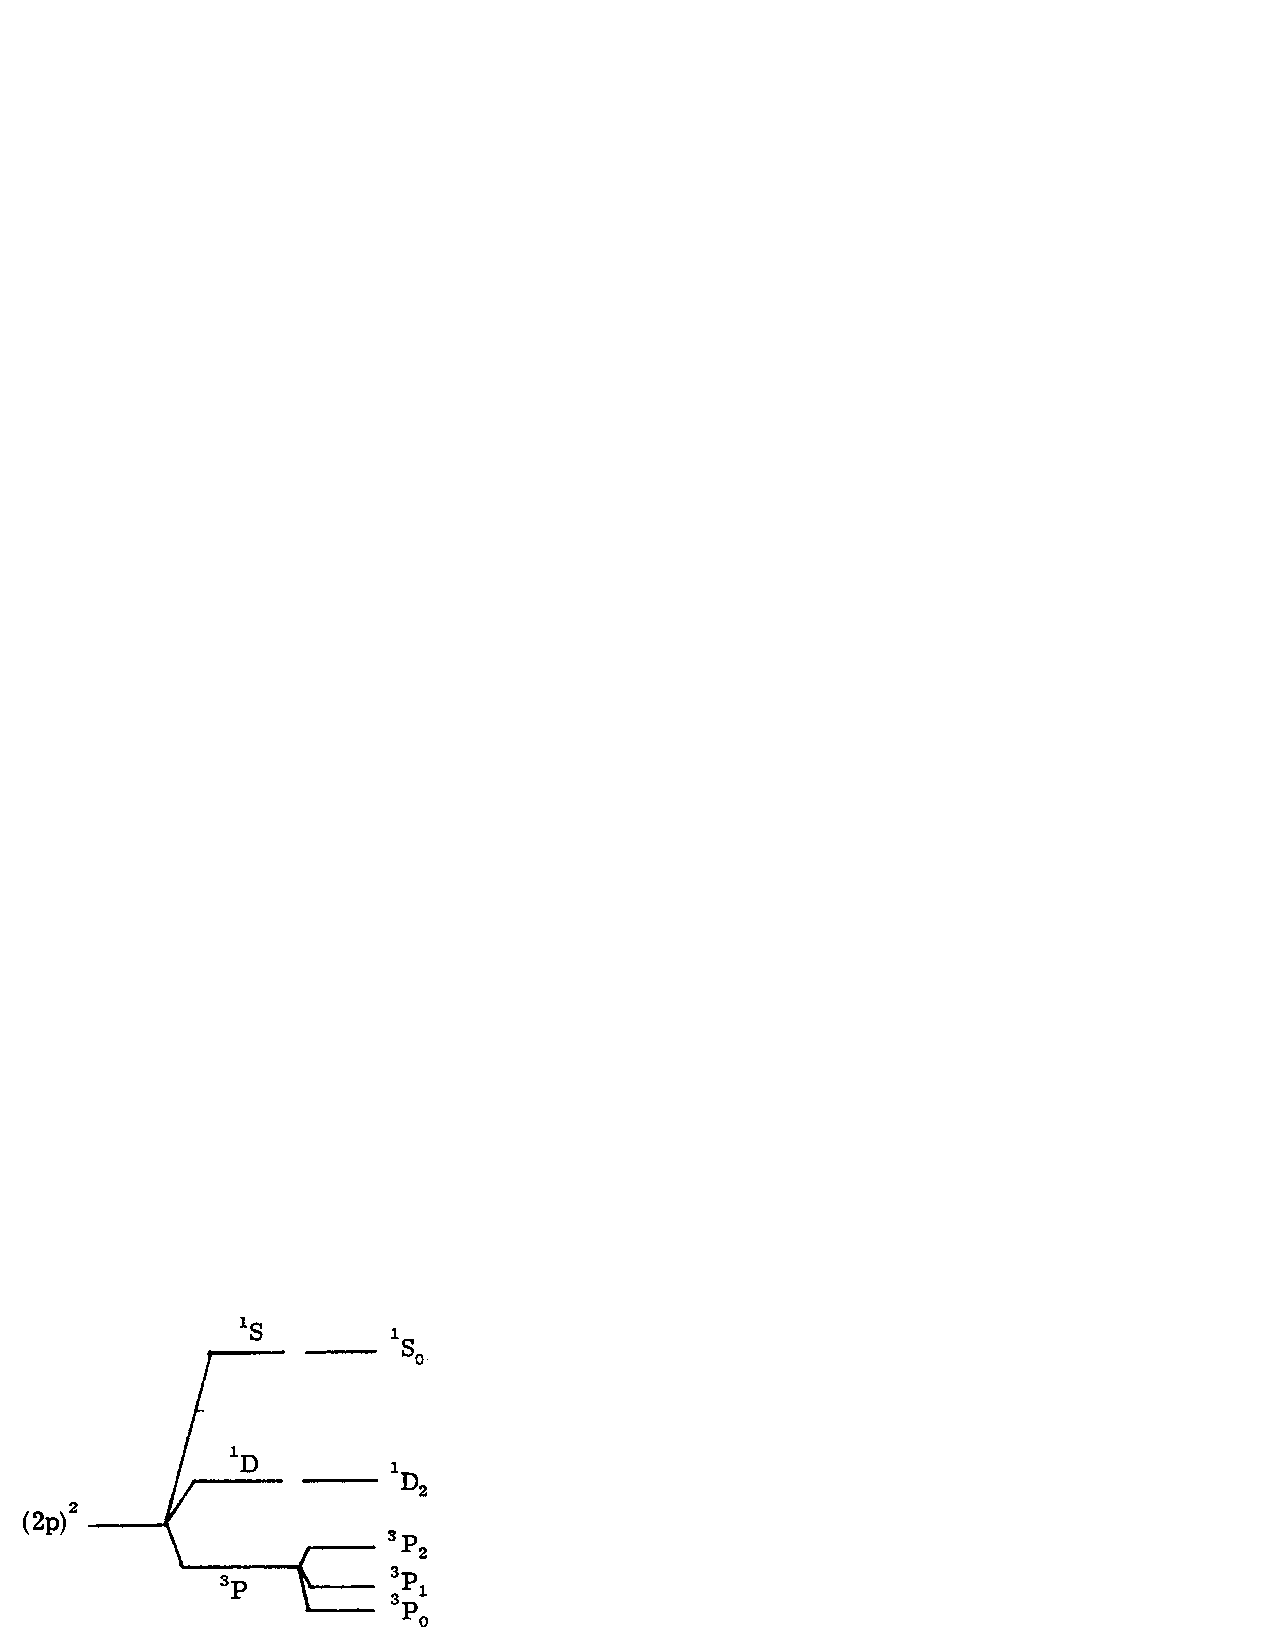
\includegraphics[scale=0.75]{fig5-11a}
\caption{}
\label{fig5-11a}
\end{figure}

\begin{figure}
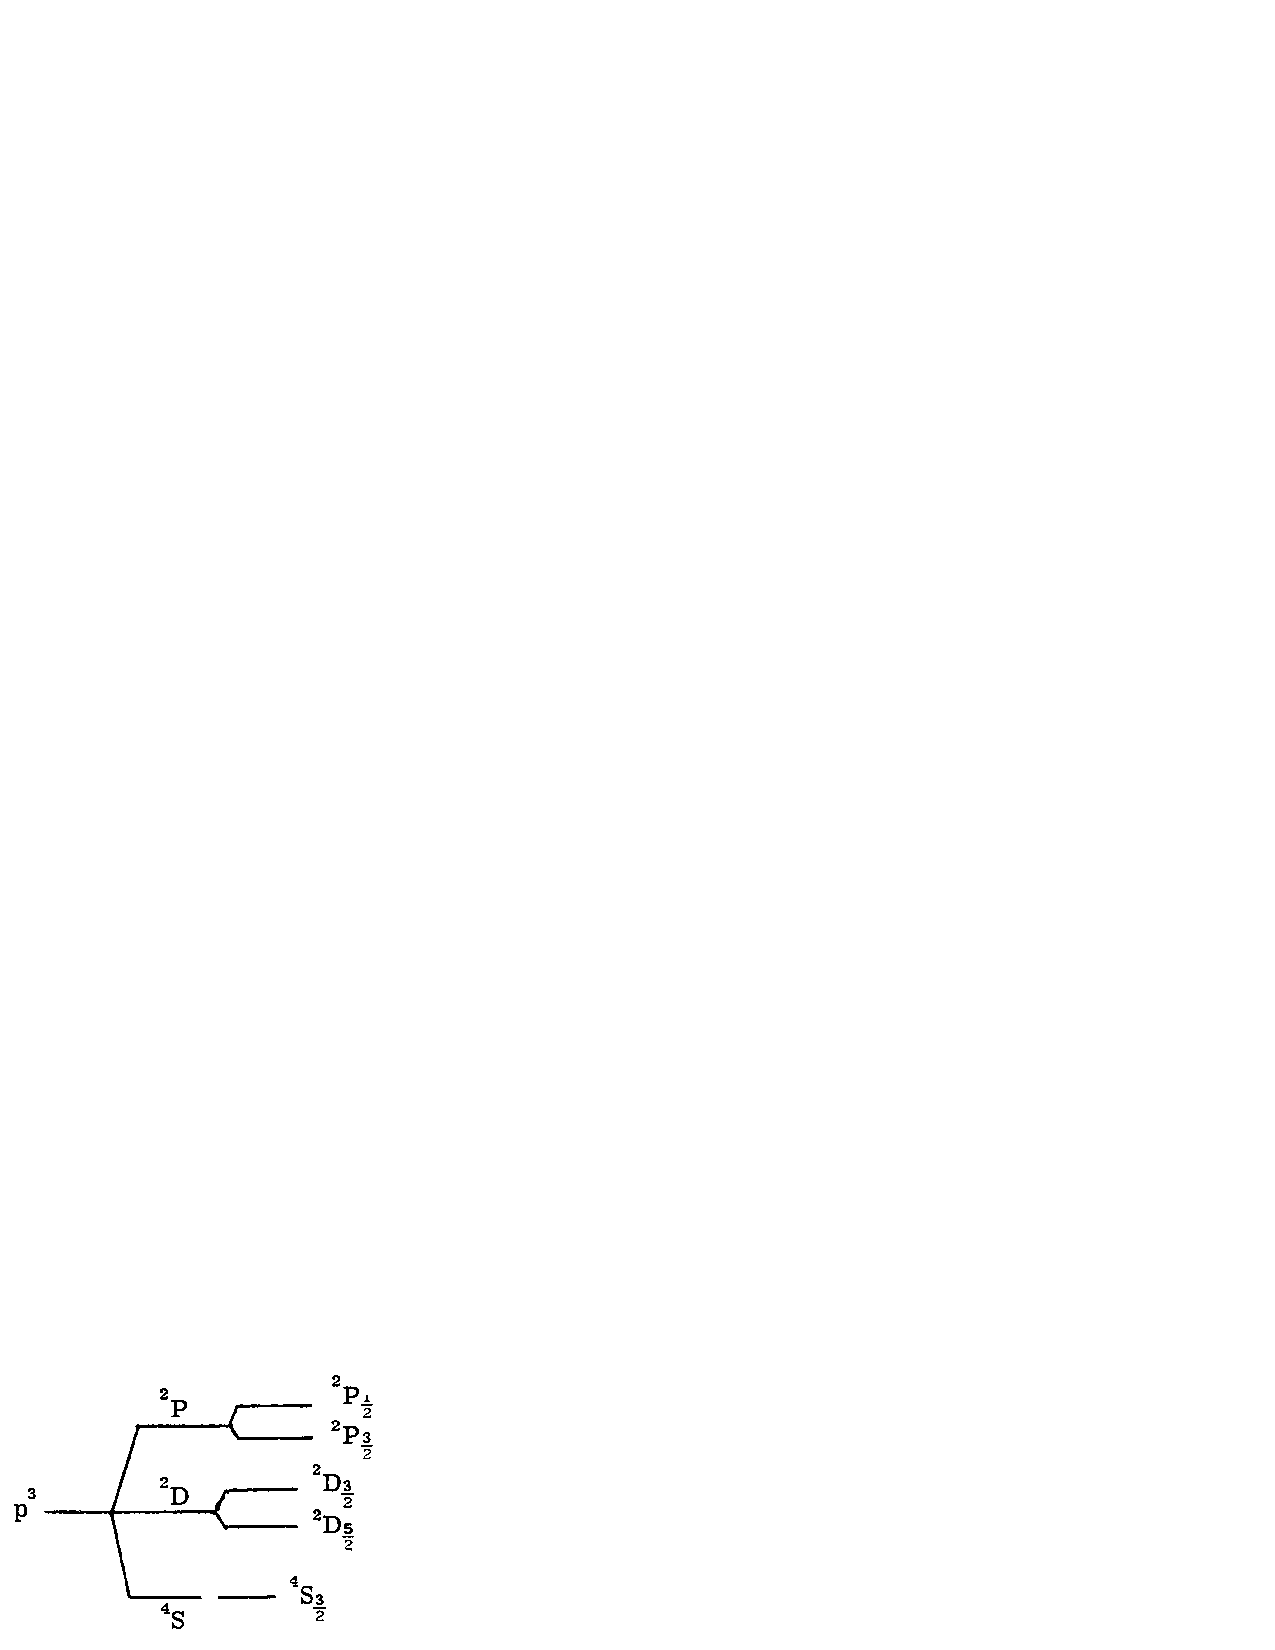
\includegraphics[scale=0.75]{fig5-11b}
\caption{}
\label{fig5-11b}
\end{figure}

Summarizing, the LS states for $p^n$ configurations are
\begin{eqnarray}
p^1 , p^5 &:& {^2P}\cr
p^2 , p^4 &:& {^3P}, {^1D} , {^1S}\cr
p^3 &:& {^4S}, {^2D}, {^2P}.
\end{eqnarray}
The allowed symmetries for various $d^n$ configurations are:
\begin{eqnarray}
d,d^9 &:& {^2D}\cr
d^2,d^3 &:& {^3F}, {^3P}, {^1G}, {^2D}, {^1S}\cr
d^3, d^7 &:& {^4F}, {^4P}, {^2H}, {^2G}, {^2F}, {^2D}, {^2D}, {^2P}\cr
d^4,d^6 &:& {^5D}, {^3H}, {^3G}, {^3F}, {^3F}, {^3D}, {^3P}, {^3P}, 
{^1I}, {^1G}, {^1G}, {^1F}, {^1D}, {^1D}, {^1S}, {^1S}\cr
d^5 &:& {^6S} , {^4G}, {^4F}, {^4D}, {^4P}, {^2I}, {^2H}, {^2G}, 
{^2G}, {^2F}, {^2D}, {^2D}, {^2D}, {^2P}, {^2S}.
\end{eqnarray}
In all cases, the ground state symmetry is listed first, but the 
higher states are not necessarily in the order given.

A useful rule for remembering which LS state is the ground state of an
atom is \emph{Hund's rule}.  Consider the configuration of orthogonal
orbitals corresponding to the ground state of an atom.
\begin{description}
\item[The $S$ rule] Of all the $LS$ eigenstates resulting from this
configuration, the lowest state is the one with the largest $S$.
\item[The $L$ rule] If there is more than one $L$ corresponding to
this largest $S$, then the lowest state is the one with the largest
$L$.  
\item[The $J$ rule] Of the various $J$ states arising from
the values of $S$ and $L$ obtained in the first two rules, the lowest
state is the one of minimum $J$, if the configuration is less than
half full, and the one of maximum $J$, configuration is more than half
full.
\end{description}

We will now examine the physical basis for Hund's rules.

\subsection{The $S$ Rule}

High spin implies symmetric spin functions.  Because of the Pauli 
principle, this implies antisymmetric spatial functions.  Since 
antisymmetric spatial functions lead to exchange integrals with negative 
signs, we see that highest spin is good, as in the first
rule. For example, the triplet state. $S = 1$, of the $xy$ configuration
\begin{equation}
{\cal A} \left[ xy \alpha \alpha \right] = \left( xy - yx \right) 
\alpha \alpha
\end{equation}
leads to
\begin{equation}
E = h_{xx} + h_{yy} + J_{xy} - K_{xy}
\end{equation}
while the single state, $S = 0$, for the configuration
\begin{equation}
{\cal A} \left[ xy \left( \alpha \beta - \beta \alpha \right) 
\right] = \left( xy + yx \right) \left( \alpha \beta - \beta \alpha 
\right)
\end{equation}
leads to an energy of
\begin{equation}
E = h_{xx} + h_{yy} + J_{xy} + K_{xy} ,
\end{equation}
$2K_{xy}$ higher than the triplet state.

The high spin state is better because the electrons in the high spin wavefunction
tend to stay further apart.  This can be seen by writing
\begin{equation}
x(1) = f ( r_1 \theta_1 ) \cos \varphi_1
\label{chap5-eqno20a}
\end{equation}
\begin{equation}
y(2) = f (r_2 \theta_2 ) \sin \varphi_2
\label{chap5-eqno20b}
\end{equation}
so that the spatial wavefunction for the triplet state is
\begin{eqnarray}
(xy-yx) &=& f(1) f(2) [ \cos \varphi_1 \sin \varphi_2 - \sin \varphi_2 
\cos \varphi_2 ]\cr
&=& f(1) f(2) \sin ( \varphi_2 - \varphi_1 )
\end{eqnarray}
whereas the spatial wavefunction for the singlet state is
\begin{equation}
(xy + yx ) = f (1) f(2) \sin ( \varphi_e + \varphi_1 ).
\end{equation}
Thus, for the triplet state, the electrons cannot have $\varphi_2 = 
\varphi_1$, and their motions are such that $\varphi_2$ and 
$\varphi_1$ tend to be at 90 degrees, with respect to each other.  On the 
other hand, there are no special $\varphi$ correlations in the singlet 
wavefunction leading to a much larger chance of $\varphi_1 \approx 
\varphi_2$.  Because the electron-electron interaction is repulsive, small 
$\varphi_2 - \varphi_1$ leads to extra repulsion resulting in a higher 
energy for the low spin state.

\subsection{The $L$ Rule}

Now we consider the second rule through use of an example.  Consider the
wavefunctions
\begin{equation}
xx - yy
\label{chap5-eqno21a}
\end{equation}
\begin{equation}
xx + yy
\label{chap5-eqno21b}
\end{equation}
having angular momenta of $M = +2$ and $M = 0$ about the $z$ axis,
both correspond to a single state.  Using
(\ref{chap5-eqno20a})--(\ref{chap5-eqno20b}), (\ref{chap5-eqno21a})
--(\ref{chap5-eqno21b}) becomes
\begin{equation}
xx - yy = f (1) f(2) \cos ( \varphi_1 + \varphi_2 )
\end{equation}
\begin{equation}
xx + yy = f (1) f(2) \cos ( \varphi_1 - \varphi_2 ).
\end{equation}
Thus, the $M = 0$ wavefunction has the $\varphi$ coordinates of the 
electrons correlated so that $\varphi_1$ and $\varphi_2$ tend to be 
equal, while the $M = 2$ wavefunction has no special correlation of 
the $\varphi$ coordinates.  Since small $\varphi_1 - \varphi_2$ leads 
to bigger electron repulsion, the $M = 2$ state is lower.  A physical 
way of thinking about this is that maximum $M$ corresponds to all 
electrons circulating in the same direction about the axis.  Thus, 
the $\varphi_1 - \varphi_2$ coordinates state fixed.  Smaller $M$ 
have the electrons circulating in opposite directions, and hence, 
$\varphi_1 - \varphi_2$ must pass through zero, leading to extra 
repulsion.

\subsection{The $J$ Rule}

In the third rule, the spin orbital coupling interaction for an atom, 
has the form
\begin{equation}
\zeta ( r ) {\bf s} \cdot {\bf l} ,
\end{equation}
where $\zeta (r) > 0$.  Thus, lower energy is obtain when {\bf s} 
and {\bf l} are in opposite directions and, hence, the best $J$ should 
be the lowest one, 
\begin{equation}
J = | L - S|,
\end{equation}
since this has the spin and orbital momenta in opposite directions.
For example, for the ${^3P}_2$ state of $p^2$, we obtain
\begin{equation}
E_{ls} = \langle p_+ p_0 \alpha \alpha | \sum_{i} \zeta ( r_i ) l_i 
\cdot s_i | {\cal A} p_+ p_0 \alpha \alpha \rangle = {1 \over 2} 
\lambda
\label{chap5-eqno22}
\end{equation}
where $\lambda$ is the radical integral
\begin{equation}
\lambda = \langle f ( r ) | \zeta ( r ) | f ( r ) \rangle
\end{equation}
and $\lambda$ is positive.

To evaluate the energy of the ${^3P}_1$ and ${^3P}_0$ terms is a 
little more complicated, but can be done using
\begin{equation}
l \cdot s = {1 \over 2} \left( {\hat l}^+ {\hat s}^- + {\hat l}^- 
{\hat s}^+ \right) + {\hat l}_z {\hat s}_z
\label{chap5-eqno23}
\end{equation}
and the usual angular momentum properties.  An alternative approach 
is to use the Wigner-Eckart theorem,
\begin{eqnarray}
E^{LSJ} &=& \langle LSJM_J | \sum_{i} \zeta ( r_i ) l_i \cdot s_i | 
LSJM_J \rangle\cr
&=& \Lambda \langle LSJM_J | L \cdot S | LSJM_J \rangle\cr
&=& {1 \over 2} \Lambda \left[ J ( J + 1 ) - S ( S + 1) - 
L(L+1)\right].
\label{chap5-eqno24}
\end{eqnarray}
Using (\ref{chap5-eqno22}) in (\ref{chap5-eqno24}), we can evaluate
$\Lambda$ as equal to  
$1/2\lambda$.  Using (\ref{chap5-eqno24}), we find that
\begin{eqnarray}
E \left( {^3P}_2 \right) &=& {1 \over 2} \lambda\cr
E \left( {^3P}_1 \right) &=& - \Lambda = - {1 \over 2} \lambda\cr
E \left( {^3P}_0 \right) &=& - 2 \Lambda = - \lambda .
\end{eqnarray}
Since $\lambda > 0$, the $J = 0$ state is lowest.

Now consider the $p^4$ configuration.  Everything is as with $p^2$ 
except that (\ref{chap5-eqno22}) is replaced by
\begin{eqnarray}
E_{ls} &= \langle p_+ p_0 p_- p_+ \alpha \alpha \alpha \beta | 
\sum_{i} \zeta ( r_i ) l_i \cdot s_i | p_+ p_0 p_- p_+ \alpha \alpha 
\alpha \beta \rangle\cr
&= {1 \over 2} \lambda - {1 \over 2} \lambda - {1 \over 2} 
\lambda = - {1 \over 2} \lambda .\cr
\end{eqnarray}
Thus,
\begin{equation}
\Lambda = -{1 \over 2} \lambda
\end{equation}
and the relationships in (\ref{chap5-eqno23}) become
\begin{eqnarray}
E \left( {^3P}_2 \right) &=& - {1 \over 2} \lambda\cr
E \left( {^3P}_1 \right) &=& {1 \over 2} \lambda\cr
E \left( {^3P}_0 \right) &=& \lambda.
\end{eqnarray}
Thus, the high $J$ state is now the ground state.  That is, with a 
greater than half-filled shell, the $M_J = J$ state, having maximum 
$M_L$ and maximum $M_S$, tends to make the unpaired spatial orbitals 
the one with most negative $M_L$.  Thus, leading to favored spin 
orbit interactions with the unpaired spins.

\subsection{Comments}

One should be careful to note what Hund's rule does not say.  It does 
not tell us which configuration is lowest, rather, given the ground 
configuration, it tells us which $LSJ$ is best.  In addition, Hund's 
rule does not tell us the sequence, or order, of the state, it only 
tells us about the ground state.  Given Hartree-Fock, or Slater 
determinant wavefunctions, Hund's rules are correct and can be 
derived, but not trivially.  However, for the exact wavefunctions, 
interactions between configurations could conceivably lead to a ground 
state in disagreement with Hund's rule, I know of no such cases.  For 
excited configurations, such interactions are often present and it is 
often the case that the sequence of excited state, having a given, 
dominant, configuration, does not satisfy Hund's rule.


\section{Appendices}

\subsection{Angular Momenta for Many-Electron Atoms}

\subsubsection{Introduction}

For a many-electron atom, the Hamiltonian is
\begin{equation}
H = \sum_{i=1}^{N} h(i) + \sum^{N}_{i>j=1} {1 \over r_{ij}}.
\end{equation}
Because of the $l/r_{ij}$ term, $l_z(i)$, the angular momentum
operator for electron $i$, does not commute with $H$.  However, the
$N$ electron operator
\begin{equation}
{\hat L}_z = \sum^{N}_{i=1} l_z(i)
\end{equation}
does commute with $H$, and similarly for $L_x$ and $L_y$.  
Consequently,
\begin{equation}
{\hat L}^2 = L^2_x + L^2_y + L^2_z
\end{equation}
also commutes with $H$, and hence, the exact eigenfunctions 
of $H$ can be taken as eigenstates of ${\hat L}^2$ and ${\hat 
L}_z$.  Similarly, we can define
\begin{equation}
{\hat S}_z = \sum^{N}_{i=1} s_z (i)
\end{equation}
and ${\hat S}^2$, both of which commute with $H$.  
Consequently, all eigenfunctions of $H$ can be taken as 
eigenstates of ${\hat L}^2$, ${\hat L}_z$, ${\hat S}^2$, and $S_z$,
\begin{eqnarray}
H \psi_{NLM_LSM_S} &=& E_{NLS} \psi_{NLM_LSM_S}\cr
{\hat L}^2 \psi_{NLM_LSM_S} &=& L(L+1) \psi_{NLM_LSM_S}\cr
{\hat L}_z \psi_{NLM_LSM_S} &=& M_L \psi_{NLM_LSM_S}\cr
{\hat S}^2 \psi_{NLM_LSM_S} &=& S(S+1) \psi_{NLM_LSM_S}\cr
{\hat S}_z \psi_{NLM_LSM_S} &=& M_S \psi_{NLM_LSM_S}.
\end{eqnarray}
In this section, we will examine how to determine the allowed values 
of $L$ and $S$, for various configurations.

\subsubsection{The $(2p)^2$ Configuration}

In Section 5.4, we contented ourselves with determining the ground 
configurations of the various atoms.  For example,
\begin{equation}
(1s)^2 (2s)^2 (2p)^2
\label{chap5app-eqno1}
\end{equation}
for $C$.  In this section, we will illustrate some ways of 
determining the possible spatial and spin symmetries for such 
wavefunctions.

Since there are three possibilities, for each of the $p$ orbitals in
(\ref{chap5app-eqno1}), and two possibilities for the spin associated
with each orbital, there are many possible wavefunctions corresponding
to (\ref{chap5app-eqno1}).  On the other hand, the total wavefunction
must satisfy Pauli's principle, restricting the possibilities.  Since
there is only one choice allowed for $(1s)^2(2s)^2$, and the essential
problem here is to determine the possible states of a configuration of
the form $(2p)^2$.

{\bf LS Eigenstates, Complex Orbitals}
Each electron is in an orbital of the form
\begin{equation}
\phi_m = f(r) Y_{1m} ( \theta , \varphi )
\end{equation}
where $m = 0, \pm 1$ is the angular momentum along the $z$ axis.

The Slater determinants, which can be formed from two $p$ orbitals, 
are as follows:
\begin{center}
\begin{tabular}{crr}\\ 
$\Psi$ & $M_L$ & $M_S$ \\
${\cal A}(p_+ p_0 \alpha \alpha)$ & +1  &  +1\cr 
${\cal A}(p_+p_- \alpha \alpha )$ & 0   &  +1\cr
${\cal A}(p_0p_- \alpha \alpha )$ & -1  &  +1\cr
${\cal A}(p_+p_+ \alpha \beta  )$ & +2  &  0 \cr
${\cal A}(p_+p_0 \alpha \beta  )$ & +1  &  0 \cr
${\cal A}(p_+p_- \alpha \beta  )$ & 0   &  0 \cr
${\cal A}(p_0p_+ \alpha \beta  )$ & +1  &  0 \cr
${\cal A}(p_0p_0 \alpha \beta  )$ & 0   &  0 \cr
${\cal A}(p_0p_- \alpha \beta  )$ & -1  &  0 \cr
${\cal A}(pp_-p_+\alpha \beta  )$ & 0   &  0 \cr
${\cal A}(pp_-p_0\alpha \beta  )$ & -1  &  0 \cr
${\cal A}(pp_-p_-\alpha \beta  )$ & -2  &  0 \cr
${\cal A}(p_+p_0\beta \beta    )$ & +1  &  -1\cr
${\cal A}(p_+p_-\beta \beta    )$ & 0   &  -1\cr
${\cal A}(p_0p_-\beta \beta    )$ & -1  &  -1\cr
\end{tabular}
\end{center}
Note that with our definition of ${\cal A}$, e.g., 
${\cal A} = e - \pi$ for $N = 2$, each wavefunction is normalized 
to $\sqrt{N!}$. We have also left out redundant states, e.g.,
\begin{equation}
{\cal A} \left( p_0 p_+ \alpha \alpha \right) - {\cal A} \left( p_+ 
p_0 \alpha \alpha \right) ,
\end{equation}
and zero determinants, e.g.,
\begin{equation}
{\cal A} \left( p_+ p_+ \alpha \alpha \right) = 0.
\end{equation}
Here, we have denoted $p_{+1}$ by $p_+$, and similarly for $p - 1$.  
Note that the above fifteen states are all orthogonal.

In terms of the $M_L$ and $M_S$ quantum numbers, these fifteen states 
are distributed as follows:
\begin{center}
\begin{tabular}{rrrrr}\\
&&\multicolumn{3}{c}{$M_S$} \\ 
&&+1 & 0 & -1 \\ \cline{3-5}
& 2 & 0 & 1 & 0 \\
& 1 & 1 & 2 & 1 \\
$M_L$ & 0 & 1 & 3 & 1 \\
& -1 & 1 & 2 & 1 \\
& -2 & 0 & 1 & 0 \\\cline{3-5}
\end{tabular}
\end{center}
Consider, first, the states with $M_S = 1$.  Since $M_S$ is maximum, 
then ${\hat S}^+$ operating on any of these states, leads to zero, and 
hence, all states with $M_S = 1$ correspond to $S = 1$.  Recall that
\begin{equation}
{\hat S}^2 = S^2_z + {\hat S}^- {\hat S}^+
\end{equation}
thus, if
\begin{equation}
{\hat S}_z \psi_M = M \psi_M
\end{equation}
and
\begin{equation}
{\hat S}^+ \psi_M = 0 ,
\end{equation}
then
\begin{equation}
{\hat S}^2 \psi_M = M ( M + 1 ) \psi_M .
\end{equation}
Now consider the maximum $M_L$ with this $M_S$, $M + L = 1$.  Since 
${\hat L}^+$ operating on this state must yield zero, we have $L = 
1$.  Thus, we find a ${^3P}$ state.  Applying ${\hat L}^-$ and ${\hat 
S}^-$, various numbers of times to the ${^3P}$ state with $M_S = 1$, 
and $M_L = 1$, leads to the nine states:
\begin{center}
\begin{tabular}{rrrrr}\\
&&\multicolumn{3}{c}{$M_S$} \\ 
&&+1 & 0 & -1 \\ \cline{3-5}
& 2 & 0 & 0 & 0 \\
& 1 & 1 & 1 & 1 \\
$M_L$ & 0 & 1 & 1 & 1 \\
& -1 & 1 & 1 & 1 \\
& -2 & 0 & 0 & 0 \\\cline{3-5}
\end{tabular}
\end{center}
Comparing this with the previous table, we see
that there are six states to be accounted for:
\begin{center}
\begin{tabular}{rrrrr}\\
&&\multicolumn{3}{c}{$M_S$} \\ 
&&+1 & 0 & -1 \\ \cline{3-5}
& 2 & 0 & 1 & 0 \\
& 1 & 0 & 1 & 0 \\
$M_L$ & 0 & 0 & 2 & 0 \\
& -1 & 0 & 1 & 0 \\
& -2 & 0 & 1 & 0 \\\cline{3-5}
\end{tabular}
\end{center}
The maximum $M_S$ for these states is $M_S =
0$, and the maximum $M_L$ is $M_L = 2$.  Thus, there must be a ${^1D}$
state.  Applying ${\hat L}^-$ successively to this $M_L = 2$ state
leads to $M_L + 1, 0 -1 , -2$ states, and comparing with
the above we see that there is one remaining state:
\begin{center}
\begin{tabular}{rrrrr}\\
&&\multicolumn{3}{c}{$M_S$} \\ 
&&+1 & 0 & -1 \\ \cline{3-5}
& 2 & 0 & 0 & 0 \\
& 1 & 0 & 0 & 0 \\
$M_L$ & 0 & 0 & 1 & 0 \\
& -1 & 0 & 0 & 0 \\
& -2 & 0 & 0 & 0 \\\cline{3-5}
\end{tabular}
\end{center}
Thus, the remaining states is ${^1S}$.  In
summary, we find $p^2 \rightarrow {^3P}, {^1D}$, and ${^1S}$.  Since
these states have degeneracies of 9, 5, and 1, respectively, we have
accounted for all fifteen states in (\ref{chap5app-eqno2}).

We will now use the ${\hat L}^-$ and ${\hat S}^-$ operators, to 
construct the many-electron wavefunctions corresponding to these states.
\begin{equation}
^3P : 
\begin{array}{lrr}\\
\Psi & M_S & M_L \\
{\cal A} \left[ p_+ \alpha p_0 \alpha \right] & 1 & 1 \\
{\cal A} \left[ p_+ \alpha p_- \alpha \right] & 1 & 0 \\
{\cal A} \left[ p_0 \alpha  p_p \alpha \right]& 1 & -1\\
{1 \over \sqrt{2}} {\cal A} \left[ \left( p_+ p_0 
- p_0 p_+ \right) \alpha \beta \right] & 0 & 1 \\
{1 \over \sqrt{2}} {\cal A} \left[ \left( p_+ p_
- p_- p_+ \right) \alpha \beta \right]& 0 & 0 \\
{1 \over \sqrt{2}} {\cal A} \left[ \left( p_0 p_-
p_- p_0 \right) \alpha \beta \right]& 0 & -1\\
{\cal A} \left[ p_- \beta p_0 \beta \right] &-1 & +1\\
{\cal A} \left[ p_+ + \alpha p_- \beta \right]&-1 & 0 \\
{\cal A} \left[ p_0 \alpha p_- \beta \right]&-1 & -1\\
\end{array}
\label{chap5app-eqno7}
\end{equation}
\begin{equation}
{^1D} : 
\begin{array}{lrr}\\
\Psi & M_S & M_L \\
{\cal A} \left[ p_+ \alpha p_+ \beta \right] & 0 &  2 \\
{1 \over \sqrt{2}} {\cal A} \left[ \left( p_+ p_0 
+ p_0 p_+ \right) \alpha \beta \right] & 0 &  1 \\
{1 \over \sqrt{6}} {\cal A} \left[ \left( 2 p_0 p_0 
+ p_+ p_- + p_- p_+ \right) \alpha \beta \right] & 0 &  0 \\
{1 \over \sqrt{2}} {\cal A} \left[ \left( p_0 p_- 
+ p_- p_0 \right) \alpha \beta \right] & 0 &  -1\\
{\cal A} \left[ p_- \alpha p_- \beta \right]& 0 &  -2\\
\end{array}
\end{equation}
For ${^1S}$, the state must be orthogonal to the $M_S = 0, M + L = 0$ 
state of ${^1D}$ and ${^3P}$.  (Note that the ${^1D}$ states and the 
${^3P}$ states are automatically orthogonal.)  Consequently
\begin{equation}
{^1S} : 
\begin{array}{lrr}\\
\Psi & M_S & M_L \\
{1 \over \sqrt{3}} {\cal A} \left[ \left( p_+ 
p_- + p_- p_+ - p_0 p_0 \right) \alpha \beta \right] &0& 0\\
\end{array}
\end{equation}

In deriving these expressions, we made use of the fact that ${\cal 
A}$ commutes with ${\hat L}^- , {\hat L}_z , {\hat S}^-$, and ${\hat 
S}_2$.  This follows since the ${\hat L}_i$ and ${\hat S}_i$ treat 
all electrons equivalently, and hence, commute with all 
permutations.  For $M_S = 0$ states, we have permuted terms so that the 
spinfunctions are in the order $\alpha \beta$.

{\bf The $J$ States}
Including spin orbital coupling, the energy eigenstates must be 
eigenfunctions of ${\hat J}^2$ and $J_z$, where ${\hat J}_i = {\hat 
L}_i + {\hat S}_i$.  For the $p^2$ states, we obtain
\begin{eqnarray}
{^3P} &:& J = 0 , 1 , 2 ,\cr
{^1D} &:& J = 2,\cr
{^1S} &:& J = 0.
\end{eqnarray}
We may recombine the nine ${^3P}$ wavefunctions of (\ref{chap5app-eqno7}) into 
eigenstates of ${\hat H}^2$ and $J_z$, using a procedure similar to 
that in Chapter 10.  Starting with $J = 2$ and $M_J = 2$, and using 
the lowering operator, lead to the following
\begin{eqnarray}
{^3P}_2 : M_J = 2 &:& {\cal A} \left[ p_+ p_0 \alpha \alpha \right]\cr
: M_J = 1 &:& {1 \over 2} {\cal A} \left[ \sqrt{2} p_+ p_- \alpha 
\alpha + \left( p_+ p_0 - p_0 p_+ \right) \alpha \beta \right]\cr
: M_J = 0 &:& {1 \over \sqrt{6}} {\cal A} \left[ p_0 p_- \alpha 
\alpha + \sqrt{2} \left( p_+ p_- + p_- p_+ \right) \alpha \beta + p_+ 
p_0 \beta \beta \right]\cr
: M_J = - 1 &:& {\cal A} \left[ (p_0 p_- - p_-p_0)\alpha\beta
+\sqrt{2}p_+p_-\beta\beta\right]\cr
: M_J = - 2 &:& {\cal A} \left[ p_0 p_-\beta\beta \right] .
\end{eqnarray}
To obtain the $J = 1$ states, we consider the $M_J = 1$ solution 
orthogonal to the above case, and then apply ${\hat J}^-$ to obtain 
the other two components, leading to the following
\begin{eqnarray}
{^3P}_1 : M_J = 1 &:& {1 \over 2} {\cal A} \left[ \sqrt{2} p_+p_- 
\alpha \alpha - \left( p_+ p_0 - p_0 p_+ \right) \alpha \beta 
\right]\cr
M_J = 0 &:& {1 \over \sqrt{2}} {\cal A} \left[ p_0 p_- \alpha 
\alpha - p_+ p_0 \beta \beta \right]\cr
M_J = - 1 &:& {\cal A} \left[ p_0 p_- - p_- p_0 \alpha \beta - \sqrt{2} 
p_+ p_- \beta \beta \right] .
\end{eqnarray}
Constructing a third $M + J = 0$ state orthogonal to the above two, 
leads to the following
\begin{equation}
{^3P}_0 : {1 \over \sqrt{6}} {\cal A} \left[ \sqrt{2} p_0 p_- \alpha 
\alpha - \left( p_+ p_- - p_- p_+ \right) \alpha \beta + \sqrt{2} p_+ 
p_0 \beta \beta \right] .
\end{equation}

More generally, we may write these $J$ states as $|LSJM_J \rangle$, 
and the original $LS$ states as $|LSM_LM_S \rangle$.  Then
\begin{equation}
|LSJM_J \rangle = \sum_{M_L,M_S} C^{LS}_{JM_J,M_L,M_S} | LSM_LM_S 
\rangle
\end{equation}
where the $C^{LS}_{JM_J,M_L,M_S}$ are the Clebsch-Gordon coefficients, 
also called the vector addition, or Wigner coefficients.  Tabulations 
are found in many references.$^1$

{\bf LS Eigenstates, Real Orbitals}
The above analysis of $L, S , J$ eigenstates, was greatly facilitated 
because the orbitals used are eigenstates of ${\hat l}_z$
\begin{equation}
{\hat l}_z Y_{lm} = mY_{lm} .
\label{chap5app-eqno8}
\end{equation}
For molecular problems, the spherical symmetry of the atom is lost 
and the complex functions of (\ref{chap5app-eqno8}) are generally not
appropriate.  For  
example, in ${\bf D}_{2h}$ symmetry, the $p$ state is split into 
$p_x , p_y$ and $p_z$ states, each with different symmetry, and hence, 
generally with different energy.  Thus, for molecular considerations, 
it is generally useful to rewrite the $LS$ eigenstates in terms of 
real wavefunctions
\begin{equation}
f(r) Z_{lm} ( \theta , \varphi ) .
\end{equation}
Starting with the complex functions, as above, this can be done by 
expanding each wavefunction, using
\begin{eqnarray}
\phi_{p_{+1}} &=& - {1 \over \sqrt{2}} \left( \phi_{px} + i \phi_{py} 
\right)\cr
\phi_{p_{-1}} &=& {1 \over \sqrt{2}} \left( \phi_{px} - i \phi_{py} 
\right)\cr
\phi_{p_0} &=& \phi_{pz} ,
\end{eqnarray}
and recombining the resulting two-electron wavefunctions.  A faster 
procedure is to note that the spatial part of the ${^3P}$ state is 
permutationally antisymmetric
\begin{equation}
\begin{array}{c}
\fbox{1}\\
\fbox{2}
\end{array}
\end{equation}
and hence, only
\begin{eqnarray}
\Phi^P_x &=& {1 \over \sqrt{2}} \left( \phi_y \phi_z - \phi_z \phi_y 
\right)\cr
\Phi^P_y &=& {1 \over \sqrt{2}} \left( \phi_z \phi_z - \phi_x \phi_z 
\right)\cr
\Phi^P_z &=& {1 \over \sqrt{2}} \left( \phi_x \phi_y - \phi_y \phi_x 
\right) .
\label{chap5app-eqno9}
\end{eqnarray}
correspond to $L = 1$.  Combining this with the three $S = 1$ spin 
functions, leads to the nine ${^3P}$ states in
(\ref{chap5app-eqno12}).  The ${^1D}$  
and ${^1S}$ states have permutationally symmetric 
\begin{equation}
\begin{array}{c}
\fbox{1}\fbox{2}
\end{array}
\end{equation}
spatial functions.  Of these, the combination
\begin{eqnarray}
\Phi^S &=& {1 \over \sqrt{3}} \left[ \phi_x (1) \phi_x (2) + \phi_y 
(1) \phi_y (2) + \phi_z (1) \phi_z (2) \right]\cr
&=& {1 \over \sqrt{3}} \left[ \phi_x \phi_x + \phi_y \phi_y + \phi_z 
\phi_z \right]
\label{chap5app-eqno10}
\end{eqnarray}
is invariant under any rotation leading to the $L = 0$, or $S$, 
state.  Thus, the other five symmetric functions
\begin{eqnarray}
\Phi^D_{z^2} &=& {1 \over \sqrt{6}} \left[ 2 \phi_z \phi_z - \phi_x 
\phi_x - \phi_y \phi_y \right]\cr
\Phi^D_{x^2-y^2} &=& {1 \over \sqrt{2}} \left[ \phi_x \phi_x - \phi_y 
\phi_y \right]\cr
\Phi^D_{xy} &=& {1 \over \sqrt{2}} \left[ \phi_x \phi_y + \phi_y 
\phi_x \right]\cr
\Phi^D_{xz} &=& {1 \over \sqrt{2}} \left[ \phi_x \phi_z + \phi_z 
\phi_x \right]\cr
\Phi^D_{yz} &=& {1 \over \sqrt{2}} \left[ \phi_y \phi_z + \phi_z 
\phi_y \right]
%
\label{chap5app-eqno11}
\end{eqnarray}
describe the $L = 2$, or $D$ state.  Summarizing, in terms of real 
functions, the fifteen states of $(p^2)$ are as follows

\begin{equation}
\begin{array}{rrl}\\
{^3P} & 1 & {\cal A} \left( p_x p_y \alpha \alpha \right)\cr
&& {\cal A} \left( p_x p_z \alpha \alpha \right)\cr
&& {\cal A} \left( p_y p_z \alpha \alpha \right)\cr
&0 & {1 \over \sqrt{2}} {\cal A} \left[ p_x p_y \left( 
\alpha \beta + \beta \alpha \right) \right] = {1 \over \sqrt{2}} 
{\cal A} \left[ \left( p_x p_y - p_y p_x \right) \alpha \beta 
\right]\cr 
&&{1 \over \sqrt{2}} {\cal A} \left[ p_x p_z \left( \alpha \beta 
+ \beta \alpha \right) \right] = {1 \over \sqrt{2}} 
{\cal A} \left[ \left( p_x p_z - p_z p_x \right) \alpha \beta 
\right]\cr 
&&{1 \over \sqrt{2}} {\cal A} \left[ p_y p_z \left( \alpha 
\beta + \beta \alpha \right) \right] = {1 \over \sqrt{2}} {\cal A} 
\left[ \left( p_y p_z - p_z p_y \right) \alpha \beta \right]\cr
& -1 & {\cal A} \left( p_x p_y \beta \beta \right)\cr
&& {\cal A} \left( p_x p_z \beta \beta \right)\cr
&& {\cal A} \left( p_y p_z \beta \beta \right)\cr
{^1D} & & {1 \over \sqrt{2}} {\cal A} \left[ \left( p_x p_x -  
p_y p_y \right) \alpha \beta \right]\cr
&& {1 \over \sqrt{2}} {\cal A} \left[ \left( p_x p_y +  
p_y p_x \right) \alpha \beta \right]\cr
&& {1 \over \sqrt{2}} {\cal A} \left[ \left( p_x p_z +  
p_z p_x \right) \alpha \beta \right]\cr
&& {1 \over \sqrt{2}} {\cal A} \left[ \left( p_y p_z +  
p_z p_y \right) \alpha \beta \right]\cr
&& {1 \over \sqrt{6}} {\cal A} \left[ \left( 2 p_z p_z -  
p_x p_x - p_y p_y \right) \alpha \beta \right]\cr
{^1S} && {1 \over \sqrt{3}} {\cal A} \left[ \left( p_x p_x +  
p_y p_y + p_z p_z \right) \alpha \beta \right]
\end{array}
\end{equation}
Note that in terms of real orbitals, only the $M_S = \pm 1$ 
components of ${^3P}$ can be written as single Slater determinants, 
whereas for the complex form, the $M_L = \pm 2$ components of ${^1D}$ 
could also be written as single Slater determinants.

{\bf Energies for $(2p)^2$ Wavefunctions}

In the following appendix, we evaluate the energies of the $p^2$ 
states.  The result is
\begin{eqnarray}
E \left( {^3P} \right) &=& h_{xx} + h_{yy} + J_{xy} - K_{xy}\cr
&=& {2 \over 3} h^0 + {1 \over 6} J^0 - {1 \over 6} K^0\cr
E \left( {^1D} \right) &=& h_{xx} + h_{yy} + J_{xy} + K_{xy}\cr
&=& h_{xx} + h_{yy} + J_{xx} - K_{xy}\cr
&=& {2 \over 3} h^0 + {1 \over 10} J^0 + {1 \over 30} K^0\cr
E \left( {^1S} \right) &=& h_{xx} + h_{yy} + J_{xx} + 2K_{xy}\cr
&=& {2 \over 3} h^0 + {1 \over 3} K^0
\label{chap5app-eqno15}
\end{eqnarray}
where
\begin{eqnarray}
h^0 &=& \sum^{3}_{i=1} h_{ii}\cr
J^0 &=& \sum^{3}_{i,j=1} J_{ij}\cr
K^0 &=& \sum^{3}_{i,j=1} K_{ij}
\label{chap5app-eqno16}
\end{eqnarray}

The expressions in (\ref{chap5app-eqno15}) are obtained directly from
the wavefunctions.  These qualities have been rewritten in terms of
the spherical invariants, by which we mean that the quantities are
each invariant under any rotation about the origin.  From
(\ref{chap5app-eqno15}) we see that the general energy expression is
\begin{equation}
E = fh^0 + aJ^0 + b K^0
\end{equation}
and hence, the variational Hamiltonian is
\begin{equation}
H = fh + 2a \sum_{j} J_j + 2b \sum_{j} K_j .
\end{equation}
This Hamiltonian is invariant under all rotations, and hence, its 
eigenstates are spherical harmonics
\begin{equation}
H \phi_i = \epsilon_i \phi_i
\end{equation}
\begin{equation}
\phi_i = f_i (r) Z_{lm} \left( \theta , \varphi \right) .
\end{equation}

Using (\ref{chap5app-eqno15}), or (\ref{chap5app-eqno16}), we see that
\begin{equation}
{E({^1S}) - E({^1D}) \over E( {^1D} ) - E ( {^3P})} = 
{3K_{xy} \over 2K_{xy}} = {3 \over 2}
\end{equation}
with $E( {^1S} ) > E( {^1D} ) > E( {^3P} )$.  Thus, the energy diagram is as 
in Figure \ref{fig5-a-1}.
\begin{figure}
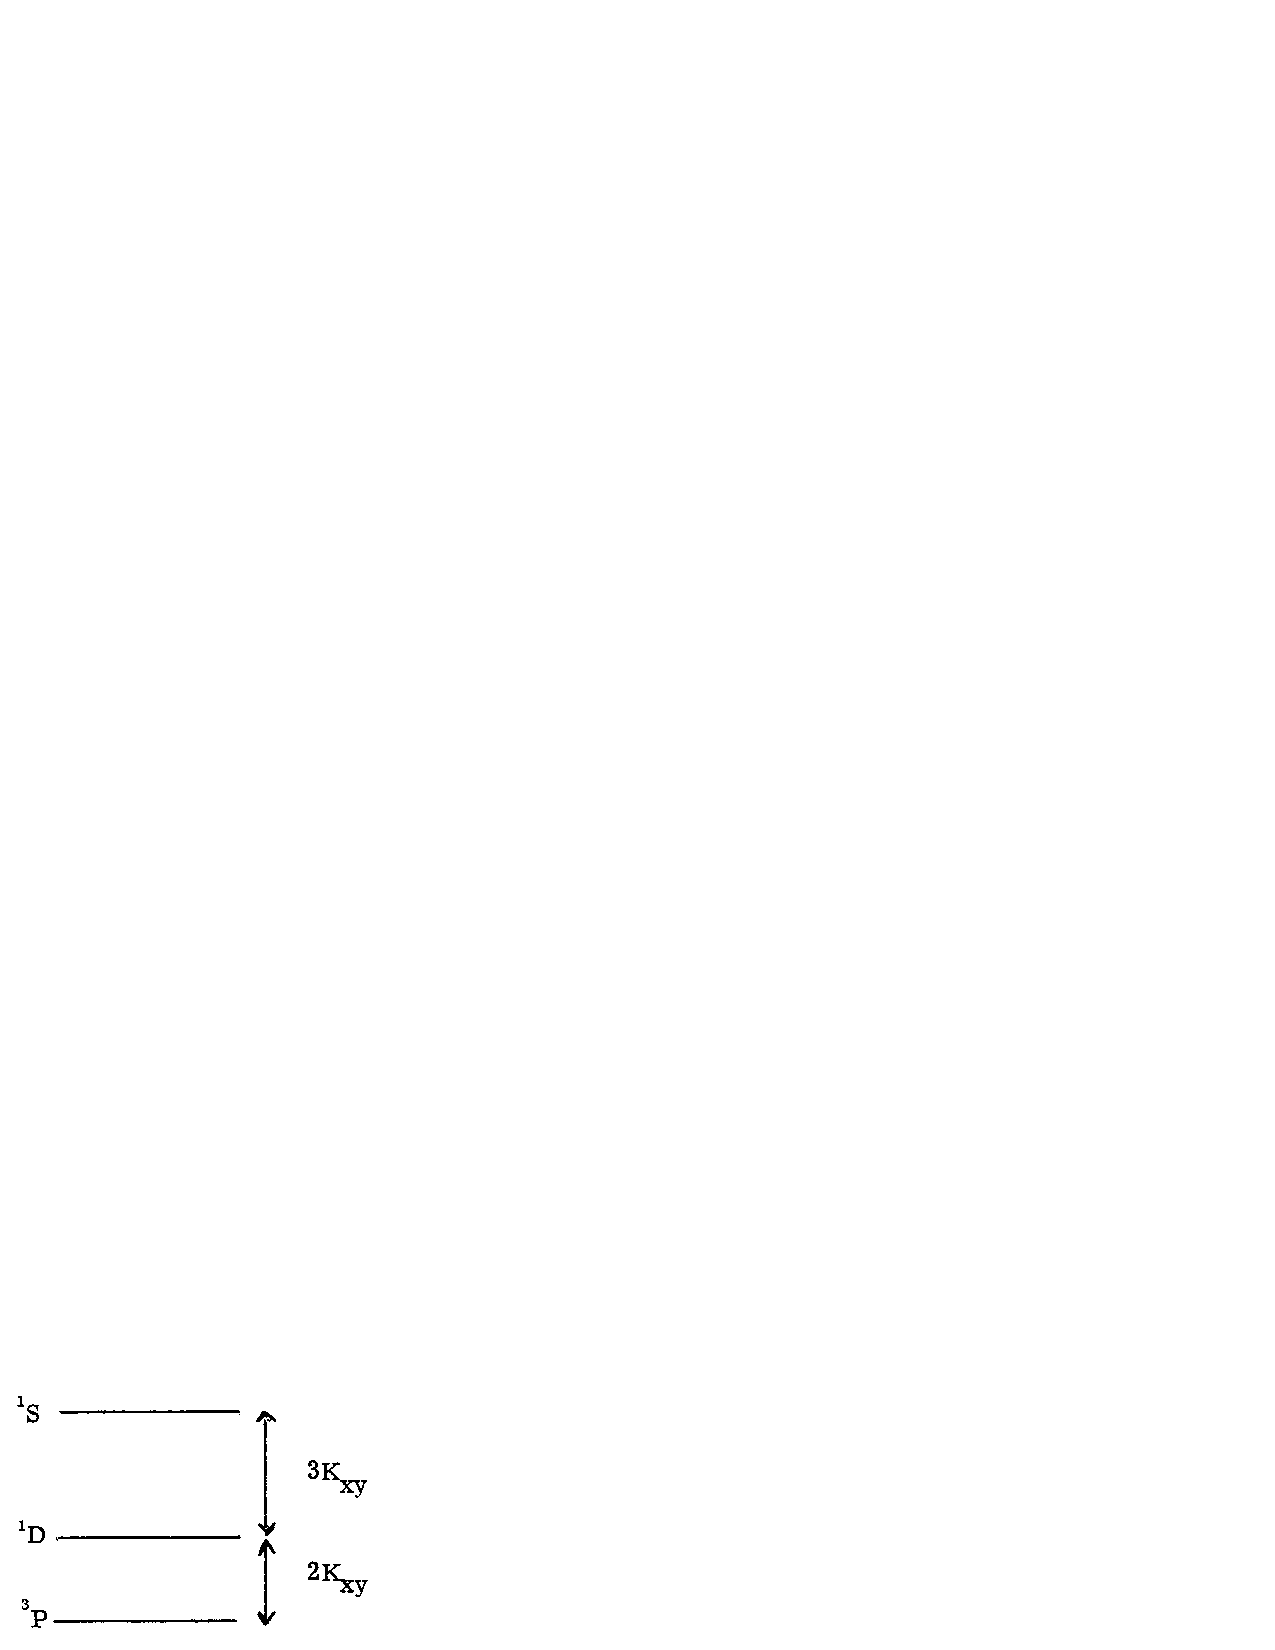
\includegraphics[scale=0.75]{fig5-12}
\caption{}
\label{fig5-a-1}
\end{figure}

\noindent
Figure \ref{fig5-a-1} is the energy diagram for $(p)^2$.

\subsubsection{Other $(2p)^n$ Configurations}

{\bf More Than Half-filled Configurations}
Consider a $(p)^4$ configuration, as the O atom.  There are six spin 
orbitals to be occupied, $p_+ \alpha , p_0 \alpha , p_- \alpha , p_+ 
\beta , p_0 \beta$, and $p_- \beta$, of which we will occupy four.  
For example,
\begin{equation}
{\cal A} \left( p_+ p_0 p_- p_+ \alpha \alpha \alpha \beta \right).
\end{equation}
All together, we find 15 such wavefunctions, each of which 
corresponds exactly to one of the 15 $p^2$ functions in
(\ref{chap5app-eqno2}).   
This correspondence is as follows
\begin{equation}
{\cal A} \left( p_+ p_0 p_- p_+ \alpha \alpha \alpha \beta \right) 
\leftrightarrow {\cal A} \left( p_0 p_- \beta \beta \right)
\end{equation}
\begin{equation}
{\cal A} \left( p_+ p_0 p_0 p_- \alpha \alpha \beta \beta \right) 
\leftrightarrow {\cal A} \left( p_- p_+ \alpha \beta \right),
\end{equation}
etc.  This is, considering the $p^4$ configuration, we identify which
two spin orbitals are not occupied (that is, the \emph{holes}) and it
is the two-electron configuration with only these holes occupied that
corresponds to the $p^4$ configuration.  Since the $M_L$ for the $p^2$
configuration has the same symmetries as a $p^2$ configuration, that
is
\begin{equation}
p^4 \rightarrow {^3P} , {^1D}, {^1S} .
\end{equation}

{\bf Summary}
The allowed symmetries for various $p^n$ configurations are listed as 
follows
\begin{eqnarray}
p^1 , p^5 &:& {^2P}\cr
p^2 , p^4 &:& {^3P}, {^1D}, {^1S}\cr
p^3 &:& {^4S} , {^2D} , {^2P}
\end{eqnarray}

\subsubsection{The $(d)^n$ Configurations}

The general procedure of obtaining the allowed $L$ and $S$ values, 
for a configuration is 
\begin{enumerate}
\item Find the number of orthogonal 
determinants allowed for each $M_S \geq 0$ and $M_L \geq 0$.  
\item Start with the largest allowed $M_S$ and with the largest $M_L$ for 
this $M_S$.  Since ${\hat L}^+$ and ${\hat S}^+$ on these states must 
both lead to zero, these states have $L = M_L$ and $S = M_S$.  
\item Considering the increases in the numbers of state for smaller $M_L$, 
we find the other $L$ states allowed for $S = M_S$.  
\item Consider the next largest $M_S$, starting with the larges allowed $M_L$. 
\item Continue this procedure until all states are 
considered.  
\end{enumerate}
We will illustrate the process once more, for the $(d^3)$ 
configuration.

{\bf The $(d^3)$ Configurations}
We find (using an obvious shorthand notation)
\begin{equation}
\begin{array}{rrl}\\
M_S & M_L & \mathrm{State} \\
3/2 & 3 & \left( 2^{\alpha} 1^{\alpha} 0^{\alpha} \right)\cr
& 2 & \left( 2^{\alpha} 1^{\alpha} {\bar{1}}^{\alpha} \right)\cr
& 1 & \left( 2^{\alpha} 0^{\alpha} {\bar{1}}^{\alpha} , 2^{\alpha} 
1^{\alpha} {\bar{1}}^{\alpha} \right)\cr
& 0 & \left( 1^{\alpha} 0^{\alpha} {\bar{1}}^{\alpha} \right) , 
\left( 2^{\alpha} 0^{\alpha} {\bar{1}}^{\alpha} \right)\cr

1/2 & 5 & \left( 2^{\alpha} 1^{\alpha} 2^{\beta} \right),\cr
& 4 & \left( 2^{\alpha} 0^{\alpha} 2^{\beta} \right) , 
\left( 2^{\alpha} 1^{\alpha} 1^{\beta} \right),\cr
& 3 & \left( 2^{\alpha} {\bar 1}^{\alpha} 2^{\beta} \right) , 
\left( 1^{\alpha} 0^{\alpha} 2^{\beta} \right), 
\left( 2^{\alpha} 0^{\alpha} 1^{\beta} \right), 
\left( 2^{\alpha} 1^{\alpha} 0^{\beta} \right) ,\cr
& 2 & \left( 2^{\alpha} {\bar 2}^{\alpha} 2^{\beta} \right) , 
\left( 1^{\alpha} {\bar 1}^{\alpha} 2^{\beta} \right) , 
\left( 2^{\alpha} {\bar 1}^{\alpha} 1^{\beta} \right) , 
\left( 1^{\alpha} 0^{\alpha} 1^{\beta} \right) , 
\left( 2^{\alpha} 1^{\alpha} {\bar 1}^{\beta} \right)\cr
& 1 & \left( 1^{\alpha} {\bar 2}^{\alpha} 2^{\beta} \right) , 
\left( 0^{\alpha} {\bar 1}^{\alpha} 2^{\beta} \right) , 
\left( 2^{\alpha} {\bar 2}^{\alpha} 1^{\beta} \right) , 
\left( 1^{\alpha} {\bar 1}^{\alpha} 1^{\beta} \right) ,\cr
&& \left( 2^{\alpha} {\bar 1}^{\alpha} 0^{\beta} \right) , 
\left( 1^{\alpha} 0^{\alpha} 0^{\beta} \right) , 
\left( 2^{\alpha} 0^{\alpha} {\bar 1}^{\beta} \right) , 
\left( 2^{\alpha} 1^{\alpha} {\bar 2}^{\beta} \right)\cr
& 0 & \left( 0^{\alpha} {\bar 2}^{\alpha} 2^{\beta} \right) , 
\left( 1^{\alpha} {\bar 2}^{\alpha} 1^{\beta} \right) , 
\left( 0^{\alpha} {\bar 1}^{\alpha} 1^{\beta} \right) , 
\left( 2^{\alpha} {\bar 2}^{\alpha} 0^{\beta} \right) ,\cr
&& \left( 1^{\alpha} {\bar 1}^{\alpha} 0^{\beta} \right) , 
\left( 2^{\alpha} {\bar 1}^{\alpha} {\bar 1}^{\beta} \right) , 
\left( 1^{\alpha} 0^{\alpha} {\bar 1}^{\beta} \right) , 
\left( 2^{\alpha} 0^{\alpha} {\bar 2}^{\beta} \right).\cr
\end{array}
\end{equation}
Therefore, we obtain the numbers in Figure \ref{fig5-a-2}, for $d^3$.

\begin{figure}
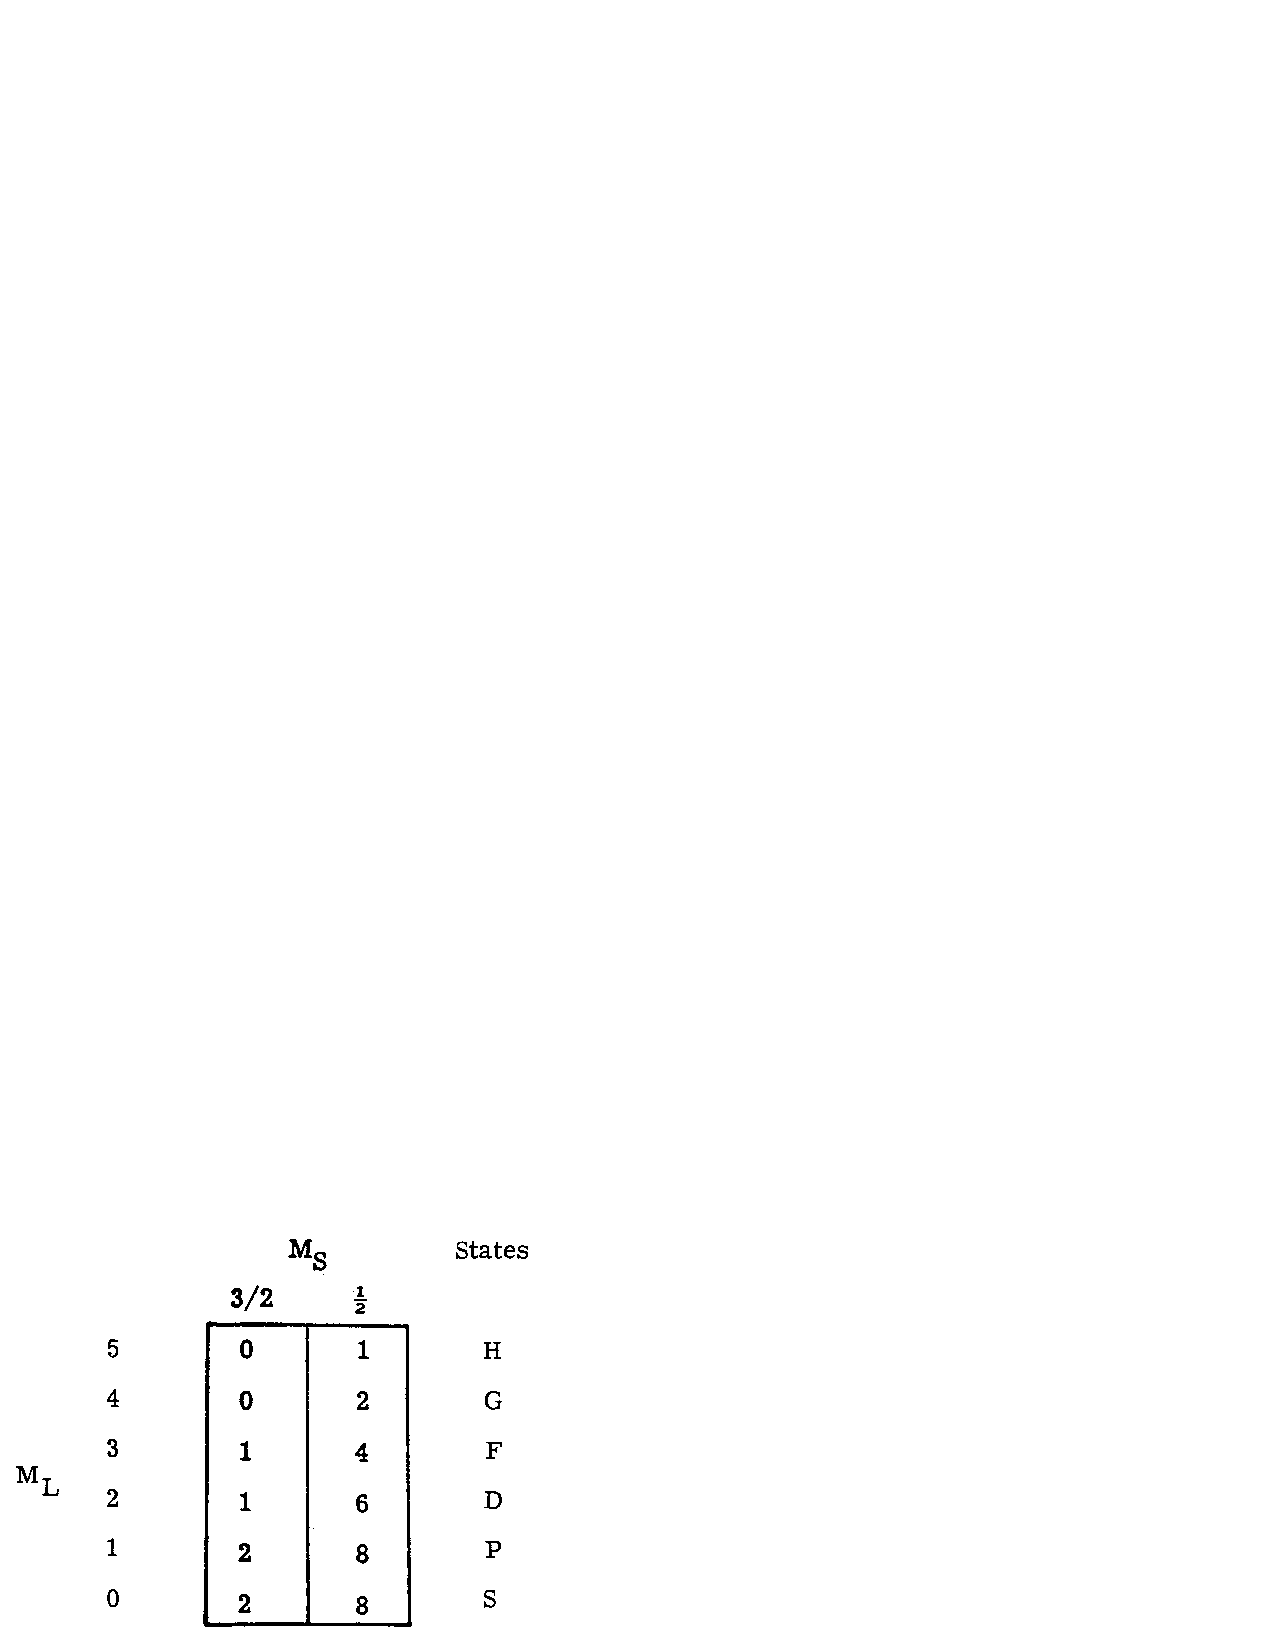
\includegraphics[scale=0.75]{fig5-13}
\caption{}
\label{fig5-a-2}
\end{figure}

\begin{enumerate}
\item Consider $M_S = 3/2$.  From $M_L = 3$ we know that we have 
one ${^4F}$, since there are one fewer states after applying ${\hat 
L}^+$.  Thus, 
\begin{enumerate}
\item $M_L = 3$ must have one ${^4F}$;  
\item $M_L = 2$ no new states, since we obtain the same number after
  applying ${\hat L}^+$;  
\item $M_L = 1$ must have one ${^4P}$;
\item $M_L = 0$ no new states.
\end{enumerate}

\item Now consider $M_S = 1/2$: 
\begin{enumerate}
\item $M_L = 5$ we have one ${^2H}$;  
\item $M_L = 4$ we have one ${^2G}$;  
\item $M_L = 3$ we have $F$ states, 
since there are two fewer after applying ${\hat L}^+$. But we already 
have one ${^4F}$, therefore we must also have one ${^2F}$. 
\item $M_L = 2$, two $D$ states and both are ${^2D}$ since there is no 
${^4D}$.  
\item $M_L = 1$ two $p$ states, applying ${\hat L}^+$, but 
one is ${^4P}$, therefore one is ${^2P}$.  
\item $M_L = 0$, no $s$ states.
\end{enumerate}
\end{enumerate}
Therefore, the $d^3$ configuration is ${^4F} , {^4P} , {^2H}, {^2G} ,
{^2F}, {^2D}, {^2D}$, and ${^2P}$.  The check for this would be, for
$\alpha \alpha \alpha$ we have $5 \cdot 4 \cdot 3/6 = 10$ different
determinants, which checks.  And for $\alpha \alpha \beta$, we have $(5
\cdot 4/2)5 = 50$ different determinants, which also checks.

\subsubsection{Inequivalent Configurations}

Earlier we considered the $(2p)^2$ configuration and found that only
${^3P} , {^1D}$, and ${^1S}$ states are allowed by the Pauli
principle.  Consider now the case $(2p)^1(3p)^1$ so that the two
electrons are in inequivalent orbitals.  This $\phi_x \phi_x$ state
can be replaced by a permutatonally symmetric term
\begin{equation}
\phi_{2x} \phi_{3x}  + \phi_{3s} \phi_{2x}
\label{chap5app-eqno18}
\end{equation}
or an antisymmetric term
\begin{equation}
\phi_{2x} \phi_{3x} - \phi_{3x} \phi_{2x} .
\label{chap5app-eqno19}
\end{equation}
Thus, we get two wavefunctions with $S$ symmetry $(x^2 + y^2 + 
z^2)$: one using (\ref{chap5app-eqno18}) leads to a singlet state
${^1S}$, and the  
other using (\ref{chap5app-eqno19}) leads to ${^3S}$.  Similarly, the
$xy - yx$ term becomes
\begin{equation}
\left( \phi_{2x} \phi_{3y} \pm \phi_{3y} \phi_{2x} \right) - \left( 
\phi_{2y} \phi_{3x} \pm \phi_{3x} \phi_{2y} \right)
\end{equation}
which leads to ${^3P}$ and ${^1P}$.  Thus, with inequivalent orbitals, 
we obtain 
\begin{equation}
(2p)(3p) \rightarrow {^3D} , {^1D}, {^3P} , {^1P} , {^3S}, {^1S}.
\end{equation}
No states are excluded by the Pauli principle.

\subsection{Energies for $(2p)^2$ Wavefunctions}

We will not evaluate the energies for the wavefunctions.  All 
energies will involve the same one-electron contributions, $2 \langle 
p | h | p \rangle$, so we will just consider the two-electron terms.

\subsubsection{Energies Using Real Wavefunctions}

Using the real wavefunctions of equations (\ref{chap5app-eqno12})
through (\ref{chap5app-eqno14}), or (\ref{chap5app-eqno10})  
and (\ref{chap5app-eqno11}), leads to the following energies:
\begin{equation}
\begin{array}{rl}\\
\mathrm{State} & \mathrm{Energy}\\
{^3P} & J_{xy} - K_{xy} = J_{xz} - K_{xz} = J_{yz} - K_{yz} \\
{^1D} & J_{xy} + K_{xy} - J_{xz} + K_{xz} = J_{yz} - K_{yz}\\
& = {1 \over 2} \left[ J_{xx} + J_{yy} - 2 K_{xy} \right]\cr
& = {1 \over 6} \left[ 4 J_{zz} + J_{xx} + J_{yy} - 4 K_{xz} - 4 
K_{yz} + 2 K_{xy} \right]\cr
{^1S} & {1 \over 3} \left[ J_{zz} + J_{xx} + J_{yy} + 2 K_{xy} + 
2K_{xz} + 2 K_{yz} \right].\\
\end{array}
\label{chap5app-eqno22}
\end{equation}
Using symmetry, there are only three different quantities here, 
$J_{xx} , J_{xy}$, and $K_{xy}$ so that the above energies reduce to
\begin{eqnarray}
{^3D} &:&  E = J_{xy} - K_{xy}\cr
{^1D} &:&  E = J_{xy} + K_{xy} = J_{xx} - K_{xy}\cr
{^1S} &:&  E - J_{xx} + 2 K_{xy} .
\label{chap5app-eqno23}
\end{eqnarray}
Since both expressions for $E({^1D})$ must be the same, we find that 
the Coulomb and exchange integrals must be related by
\begin{equation}
J_{xx} = J_{xy} + 2 K_{xy}
\end{equation}
Consequently,
\begin{eqnarray}
{^3P} &:& E = J_{xy} - K_{xy}\cr
{^1D} &:& E = J_{xy} + K_{xy}\cr
{^1S} &:& E = J_{xy} + 4 K_{xy}
\label{chap5app-eqno24}
\end{eqnarray}
leading to
\begin{equation}
{E({^1S}) - E({^1D}) \over E({^1D}) - E({^3P})} = 
{3K_{xy} \over 2K_{xy}} = {3 \over 2}.
\label{chap5app-eqno25}
\end{equation}
Thus, since $K_{xy} > 0$, we see that the states must be in the order 
given in Figure \ref{fig5-a-3}, with the ratio of 3 to 2 in the energy 
separations.  

\begin{figure}
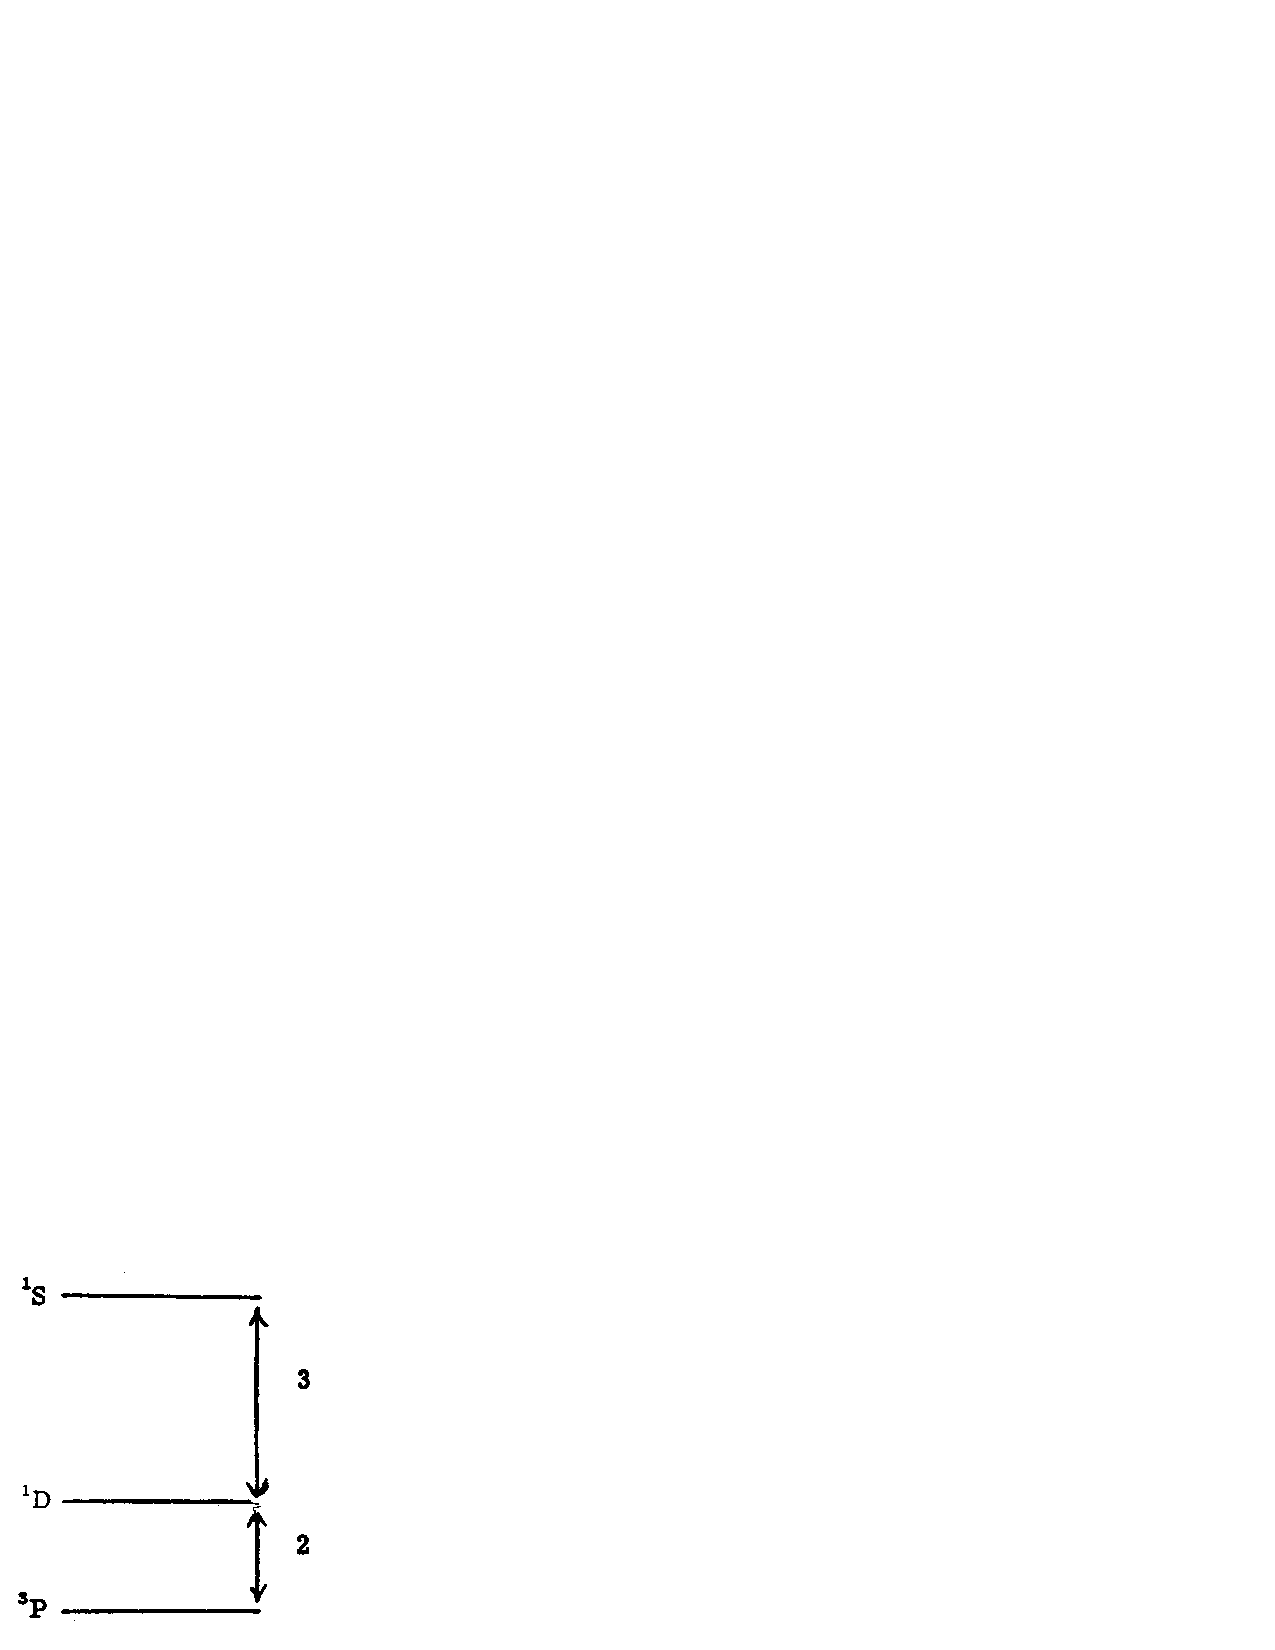
\includegraphics[scale=0.75]{fig5-14}
\caption{The energy diagram for $(2p)^2$.}
\label{fig5-a-3}
\end{figure}

\subsubsection{Spherically Averaged Energies}

The problem with the energy expressions of (\ref{chap5app-eqno20})
through (\ref{chap5app-eqno23}), or (\ref{chap5app-eqno24}),  
is that they distinguish specific directions over others. For example, 
using
\begin{equation}
E = \langle x | h | x \rangle + \langle y | h | y \rangle + J_{xy} + 
K_{xy}
\end{equation}
leads to variational operators
\begin{equation}
H_x = h + J_y + K_y
\end{equation}
and
\begin{equation}
H_y = h + J_x + K_x.
\end{equation}
Since the operators do not have spherical symmetry, the solutions are 
not spherical harmonics
\begin{equation}
\phi_u = f ( r ) Y_{lm} \left( \theta , \varphi \right) .
\end{equation}
In order to remedy this, we will average the energy expressions for 
different equivalent states.  Thus, (\ref{chap5app-eqno20}),
(\ref{chap5app-eqno21}), and (\ref{chap5app-eqno22}) lead to 
\begin{eqnarray}
E ( {^3P} ) &=& {1 \over 3} \sum_{i>j} \left( J_{ij} - K_{ij}\right)\\
E ( {^1D} ) &=& {1 \over 3} \sum_{i>j} \left( J_{ij} + K_{ij}\right) 
= {1 \over 3} \sum_{i} J_{ii} - {1 \over 3} \sum_{i>j} K_{ih}\\
E ( {^1S} ) &=& {1 \over 3} \sum_{i>j} J_{ii} + {2 \over 3} \sum_{i>j} 
K_{ij} .
\label{chap5app-eqno26}
\end{eqnarray}
Since only equal energies were averaged together, nothing has been 
changed but the appearance of the energy expression.  Going one step 
further, we add
\begin{equation}
{1 \over 6} \sum_{i} \left( J_{ii} - K_{ii} \right) = 0 ,
\label{chap5app-eqno29}
\end{equation}
to (\ref{chap5app-eqno26}), leading to
\begin{equation}
E \left( {^3P} \right) = {1 \over 6} \left( J^0 - K^0 \right)
\label{chap5app-eqno30}
\end{equation}
where
\begin{equation}
J^0 = \sum_{i,j} J_{ij}
\label{chap5app-eqno31a}
\end{equation}
and
\begin{equation}
K^0 = \sum_{i,j} K_{ij}
\label{chap5app-eqno31b}
\end{equation}
are spherically invariant.  Similarly, using (\ref{chap5app-eqno29}),
(\ref{chap5app-eqno28}) becomes 
\begin{equation}
E \left( {^1S} \right) = {1 \over 3} K^0 .
\label{chap5app-eqno32}
\end{equation}
This leads to
\begin{eqnarray}
E ( {^1D} ) &=& {1 \over 5} \sum_{i>j} \left( J_{ij} + K_{ij}\right) 
    + {2 \over 15} \sum_{i>j} \left( J_{ij} - K_{ij}\right) \cr
 &=& {1 \over 10} J^0 + {1 \over 30} K^0
\label{chap5app-eqno33}
\end{eqnarray}
Thus, we find that
\begin{equation}
E ( {^1S} ) - E ( {^1D} ) = {1 \over 10} \left( 3K^0 - J^0 \right)
\end{equation}
\begin{equation}
E ( {^1D} ) - E ( {^3P} ) = {1 \over 15} \left( 3 K^0 - J^0 \right)
\end{equation}
leading again to (\ref{chap5app-eqno25}).  Comparing to
(\ref{chap5app-eqno24}), we see that
\begin{equation}
{1 \over 15} \left( 3K^0 - J^0 \right) = 2 K_{xy} > 0 .
\end{equation}
From (\ref{chap5app-eqno30}) through (\ref{chap5app-eqno33}), we see
that for each state, the energy can be written as
\begin{equation}
E = f \sum_{i} h_{ii} + a \sum_{i,j} J_{ij} + b \sum_{i,j} K_{ij} ,
\end{equation}
where each sum is over the three $p$ functions, $f = 2/3$ for the 
$p^2$ configuration.  Thus, the variational Hamiltonian is
\begin{equation}
H = fh  + 2 a \sum_{j} J_j + 2 b \sum_{j} K_j .
\end{equation}
This operator is rotationally invariant, and hence, the eigenstates
\begin{equation}
H \phi_i = \epsilon_i \phi_i
\end{equation}
are spherical harmonics
\begin{equation}
\phi_i = f_i ( r ) Z_{lm} ( \theta , \varphi ) .
\end{equation}

\subsubsection{Energies Using Complex Orbitals}

Using complex orbitals $p_+ , p_0$, and $p_-$, the energies for the 
$p^2$ configurations are
\begin{equation}
\begin{array}{rl}
\mathrm{State} & \mathrm{Energy}\\
{^3P} & J_{+0} - K_{+0} = J_{+-} - K_{+-} = J_{0-} - K_{0-}\cr
{^1D} & J_{++} = J_{+0} + K_{+0}\cr
  &= {1 \over 6} \left( 1 J_{00} + 2J_{+-} + 2K_{+-} - 4K_{+0} - 
4K_{0+} \right)\cr
&= J_{-0} + K_{-0} = J_{--}\cr
{^1S} & {1 \over 3} \left( 2 J_{+-} + J_{00} + 2K_{+-} + 
2K_{+0} + 2K_{-0} \right)\cr
\end{array}
\end{equation}
where we have used $\phi^*_0 = \phi_0$, and
\begin{eqnarray}
\langle 0 0 | {1 \over r_{12}} | + - \rangle &= \int d 
\tau_1 \phi_0 (1) \underbrace{\phi_+(1)}_{-\phi_-(1)*} \int d \tau_2 
{1 \over r_{12}} \phi_b (2) \phi_- (2)\cr
&= - \langle - 0 | {1 \over r_{12}} | 0 - \rangle = - 
K_{0-}\cr
\end{eqnarray}

Averaging over the various components, of a state, and using $J_{++} = 
J_{--} = J_{+-}$, we obtain
\begin{equation}
\begin{array}{rl}
\mathrm{State} & \mathrm{Energy}\\
{^3P} & {1 \over 6} J^0 - {1 \over 6} K^0\cr
{^1D} & {1 \over 10} J^0 - {1 \over 30} K^0\cr
{^1S} & {1 \over 3} K^0 \\
\end{array}
\end{equation}
where
\begin{equation}
J^0 = \sum^{+1}_{m,m^{\prime}=-1} J_{mm^{\prime}}
\end{equation}
and
\begin{equation}
K^0 = \sum^{+1}_{m,m^{\prime}=-1} J_{mm^{\prime}}
\end{equation}
are the spherical invariants and are equivalent to the forms used in 
(\ref{chap5app-eqno31}).

\subsection{The Virial Theorem}

To summarize, in a system of particles interacting through a Coulomb 
potential, the total kinetic energy $T$, total potential energy $V$, 
and total energy $E$, are related as
\begin{equation}
E = - T = {1 \over 2} V.
\end{equation}
This relationship is also true for approximate wavefunctions if the 
scale of the approximate wavefunction is optimized.

\subsubsection{Coulomb Potentials}

In this chapter, we found that any approximate wavefunction yields an 
energy greater than, or equal to, the exact energy.  Hence, varying 
various parameters in the wavefunction to minimize the energy, should 
lead to better wavefunctions for the ground state.  As a corollary, we 
know that the energy of the exact wavefunction must already be a 
minimum, with respect to variation of any parameters in the 
wavefunction.  This knowledge can be used to obtain a relationship 
between the average kinetic and potential energies of a wavefunction.

Starting with some wavefunction $\phi_1(r)$, say
\begin{equation}
\phi_1 (r) = e^{-2r} \cos (3r) ,
\end{equation}
we will consider the scaled wavefunction
\begin{equation}
\phi_{\alpha} (r) = e^{-2 \alpha r} \cos \left( 3 \alpha r \right) ,
\end{equation}
obtained from $\phi_1(r)$ by replacing $r$ with $\alpha r$. This 
amounts to squeezing a wavefunction by a factor of $\alpha$, as 
indicated in Figure \ref{fig5-x-4}.  

\begin{figure}
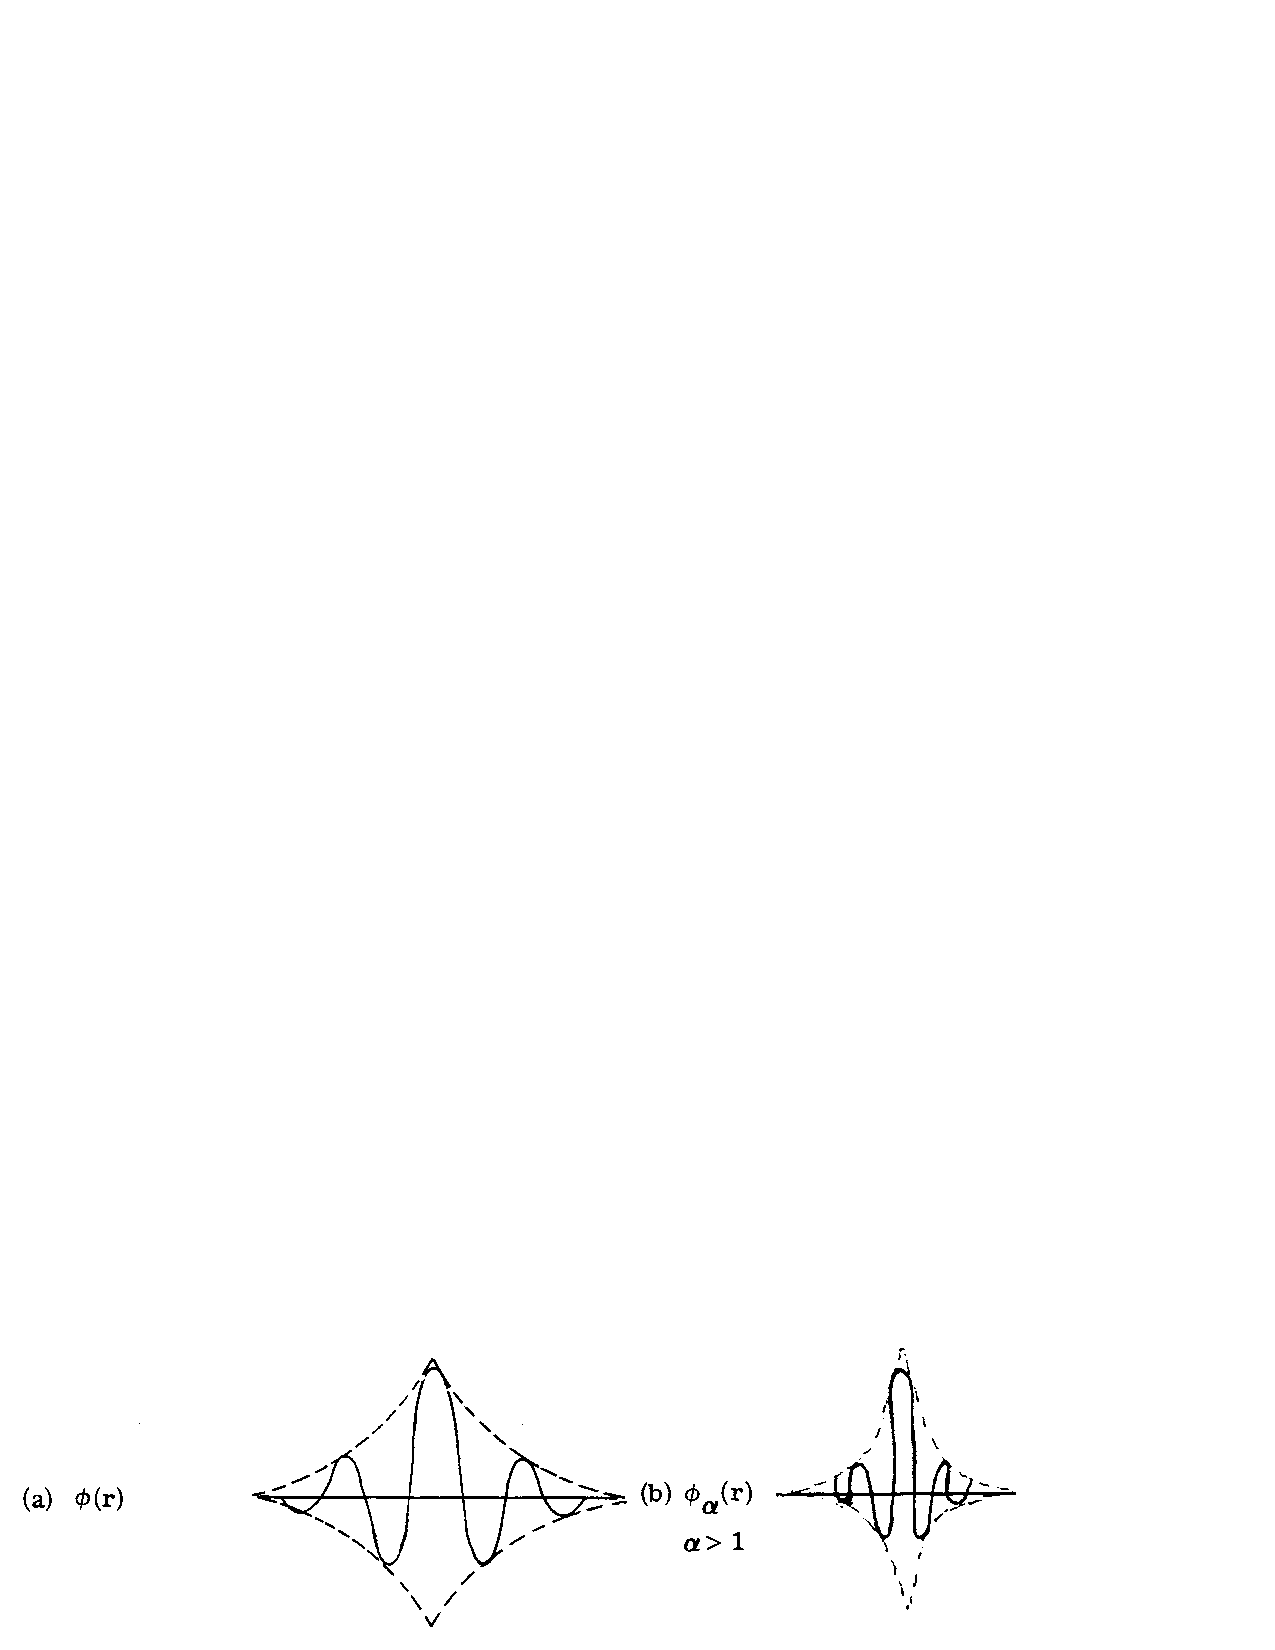
\includegraphics[scale=0.75]{fig5-c-1}
\caption{Illustration for the virial theorem.}
\label{fig5-x-4}
\end{figure}

The energy of the new wavefunction is given by
\begin{equation}
E_{\alpha} = T_{\alpha} + V_{\alpha}
\end{equation}
where
\begin{equation}
T_{\alpha} = {\langle \phi_{\alpha} | - {1 \over 2} \nabla^2 
| \phi_{\alpha} \rangle \over \langle \phi_{\alpha} | \phi_{\alpha} 
\rangle}
\end{equation}
and
\begin{equation}
V_{\alpha} = {\langle \phi_{\alpha} | - {Z \over r} | 
\phi_{\alpha} \rangle \over \langle \phi_{\alpha} | \phi_{\alpha} 
\rangle} .
\end{equation}
But
\begin{equation}
\phi_{\alpha} (r) = \phi_1 ( \alpha r )
\end{equation}
and $\phi_1(r)$ are normalized,
\begin{equation}
\langle \phi_1 | \phi_1 \rangle = \int d^3 r \phi^*_1 (4) \phi_1 (r) = 
1 ,
\end{equation}
so that
\begin{eqnarray}
\langle \phi_{\alpha} | \phi_{\alpha} \rangle &=& \int d^3 r 
\phi^*_{\alpha} (r) \phi_{\alpha} (r) = \int d^3 r \phi^*_i ( \alpha 
r ) \phi_1 ( \alpha r )\cr
&=& {1 \over \alpha^3} \int d^3 ( \alpha r ) \phi^*_1 ( \alpha r ) 
\phi_1 ( \alpha r ) = {1 \over \alpha^3} \int d^3 r^{\prime} \phi^*_1 
(r^{\prime} ) \phi_1 (r^{\prime} )\cr
&=& {1 \over \alpha^3}
\end{eqnarray}
Similarly
\begin{eqnarray}
\langle \phi_{\alpha} | - {Z \over r} | \phi_{\alpha} 
\rangle &=& \alpha \langle \phi_{\alpha} (r) | - {Z \over \alpha 
r} | \phi_{\alpha} (r) \rangle\cr
&=& {\alpha \over \alpha^3} \langle \phi_1 ( \alpha r ) | - {Z 
\over \alpha r} | \phi_1 ( \alpha r ) \rangle \cr
&=& {\alpha \over \alpha^3} V_1 ,
\end{eqnarray}
where
\begin{equation}
V_1 = \langle \phi_1 (r) | - {Z \over r} | \phi_1 (r) 
\rangle = \langle \phi_1 ( \alpha r )  | - {Z \over \alpha r} 
| \phi_1 ( \alpha r ) \rangle .
\label{chap5app-eqno34}
\end{equation}
In (\ref{chap5app-eqno34}) the two forms just differ by a change of variable 
$r^{\prime} - \alpha r$.  This does not change the boundary 
conditions, since the wavefunction is zero at $t = \infty$, and 
hence, at $r^{\prime} = \infty$, and (\ref{chap5app-eqno34}) follows.  Thus,
\begin{equation}
V_{\alpha} = \alpha V_1 .
\label{chap5app-eqno35}
\end{equation}
Similarly
\begin{equation}
T_{\alpha} = \alpha^2 T_1 ,
\label{chap5app-eqno36}
\end{equation}
so that the energy has the form
\begin{equation}
E_{\alpha} = \alpha^2 T_1 + \alpha V_1 .
\end{equation}
Requiring $E_{\alpha}$ to be a minimum with respect to the $\alpha$, 
leads to
\begin{equation}
0 = 2 \alpha T_1 + V_1
\end{equation}
or
\begin{equation}
\alpha = - {V_1 \over 2T_1}.
\label{chap5app-eqno37}
\end{equation}
Thus, from (\ref{chap5app-eqno35}) and (\ref{chap5app-eqno36}), we obtain
\begin{eqnarray}
V^\mathrm{opt} &=& - {(V_1)^2 \over 2T_1}\cr
T^\mathrm{opt} &=& + {(V_1)^2 \over 4T_1}
\end{eqnarray}
and hence,
\begin{equation}
2T^\mathrm{opt} + V^\mathrm{opt} = 0 .
\label{chap5app-eqno38}
\end{equation}
This is called the \emph{virial theorem}, and leads to
\begin{equation}
E^\mathrm{opt} = - T^\mathrm{opt} = + {1 \over 2} V^\mathrm{opt} .
\end{equation}

Since the exact eigenfunction must already be optimum with respect to 
scaling, (\ref{chap5app-eqno38}) must apply to the exact wavefunction.

\subsubsection{Other Potentials}

If, instead of the Coulomb potential,
\begin{equation}
{\hat V} = - {Z \over r} ,
\end{equation}
we consider some other homogeneous potential,
\begin{equation}
V = \beta r^n ,
\end{equation}
then the above scaling considerations, lead to
\begin{equation}
E_{\alpha} = \alpha^2 T_1 + \alpha^{-n} V_1
\end{equation}
and hence, to
\begin{equation}
2 \alpha T_1 - n \alpha^{-n-1} V_1  0
\end{equation}
in place of (\ref{chap5app-eqno37}).  This results in the general form
of the virial theorem
\begin{equation}
2 T^\mathrm{opt} = n V^\mathrm{opt}
\end{equation}
in place of (\ref{chap5app-eqno38}).  For example, a harmonic
oscillator has $n = 2$, and hence,
\begin{equation} 
T^\mathrm{opt} = V^\mathrm{opt} .
\end{equation}
